\documentclass{report}
\usepackage[utf8]{inputenc}
\usepackage{amsmath}
\usepackage{amsfonts}
\usepackage{natbib}
\usepackage{graphicx}
\usepackage{fancyhdr}
\usepackage{lmodern}
\usepackage{mathtools}
\usepackage{xcolor}
\usepackage{placeins}
\usepackage[a4paper, total={6in, 8in}]{geometry}
\usepackage{hyperref}
\hypersetup{
    colorlinks=true,
    linkcolor=black,
    filecolor=magenta,      
    urlcolor=cyan,
}

\pagestyle{fancy}
\renewcommand{\footrulewidth}{0.4pt}
\interfootnotelinepenalty=10000
\fancyhf{}
\lhead{\color{gray}{\small{IAC project by Alessio Russo, Carmelo Valore}}}
\rhead{\color{gray}{\small{\rightmark}}}
\lfoot{\textcolor{gray}{\small{MIDA2 project - mOve}}}
\rfoot{\textcolor{gray}{\normalsize{\thepage}}}

\let\Oldsection\section
\renewcommand{\section}{\FloatBarrier\Oldsection}

\let\Oldsubsection\subsection
\renewcommand{\subsection}{\FloatBarrier\Oldsubsection}

\let\Oldsubsubsection\subsubsection
\renewcommand{\subsubsection}{\FloatBarrier\Oldsubsubsection}

\title{\textbf{Dynamic bicycle model}}
\author{Alessio Russo, Carmelo Valore}
\date{\today}

\begin{document}


\begin{titlepage}
    \begin{center}
        \includegraphics[width=0.4\textwidth]{images/intro/logo.png}

		\vspace{1cm}

		\Huge
        \textbf{IAC Project}

        \vspace{0.5cm}

		\large
        Indycar Autonomous Challenge 

        \vspace{0.8cm}

 		\normalsize
        \textbf{Alessio Russo 945781\\Carmelo Valore 944851}

        \vfill

		\normalsize
        Accademic year 19/20

        \vspace{0.8cm}

		\normalsize

        \textit{Industrial and Information Engineering}\\
        \textit{Computer Science and Engineering}\\
        \textit{\today}\\

    \end{center}
\end{titlepage}

\newpage
\tableofcontents
\newpage

\chapter{Dynamic model}
In this chapter all the steps towards the realization of our model are detailed. The final model is a dynamic bycicle model that takes into consideration the non-linear tyre model using the Pacejka magic formula, the fuel consumpation, the aerodynamic forces and slipstream effect, the tyre wears and finally also the banking of the road.
\section{Simple dynamic model}

\begin{figure}[h!]
    \centering
    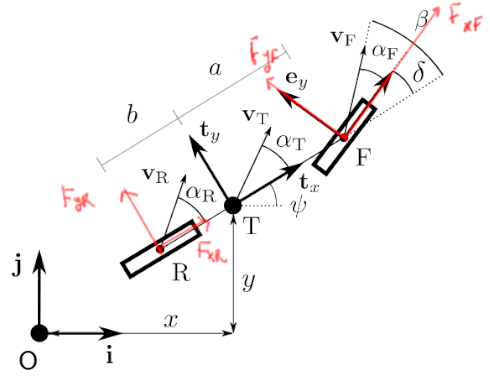
\includegraphics[scale = 0.7]{images/chapter1/im_model.png}
    \caption{Bicycle model}
    \label{fig:bmodel}
\end{figure}

\begin{equation}
\begin{aligned}
m_T \ddot{x} = F_{xF} cos(\psi+\delta) + F_{xR} cos(\psi) - F_{yF} sin(\psi+\delta) - F_{yR} sin(\psi) \\
m_T \ddot{y} = F_{xF} sin(\psi+\delta) + F_{xR} sin(\psi) + F_{yF} cos(\psi+\delta) + F_{yR} cos(\psi) \\
I_T \ddot{\psi} = F_{xF} a sin(\delta) + F_{yF} a cos(\delta) - F_{yR} b\\\\
\end{aligned}
\end{equation}

\begin{equation}
\begin{aligned}
\alpha_F = arctan(\frac{\dot{y}+a\dot{\psi}cos(\psi)}{\dot{x}-a\dot{\psi}sin(\psi)}) - (\delta + \psi)\\
\alpha_R = arctan(\frac{\dot{y}-b\dot{\psi}cos(\psi)}{\dot{x}+b\dot{\psi}sin(\psi)}) - \psi\\\\
\end{aligned}
\end{equation}

At first, as state vector this has been used:

\begin{equation}
\begin{aligned}
z1 = x\\
z2 = y\\
z3 = \psi\\
z4 = \dot{x}\\
z5 = \dot{y}\\
z6 = \dot{\psi}\\\\
\end{aligned}
\end{equation}

So that

\begin{equation}
\begin{aligned}
\dot{z_1} = z_4 \\
\dot{z_2} = z_5 \\
\dot{z_3} = z_6 \\
\dot{z_4} = \frac{F_{xF} cos(z_3+\delta) + F_{xR} cos(z_3) - F_{yF} sin(z_3+\delta) - F_{yR} sin(z_3)}{m_T} \\
\dot{z_5} = \frac{F_{xF} sin(z_3+\delta) + F_{xR} sin(z_3) + F_{yF} cos(z_3+\delta) + F_{yR} cos(z_3)}{m_T} \\
\dot{z_6} = \frac{F_{xF} a sin(\delta) + F_{yF} a cos(\delta) - F_{yR} b}{I_T} \\\\
\end{aligned}
\end{equation}

With slip angles

\begin{equation}
\begin{aligned}
\alpha_F = arctan(\frac{z_5+a z_6 cos(z_3)}{z_4-a z_6 sin(z_3)}) - (\delta + z_3)\\
\alpha_R = arctan(\frac{z_5-b z_6 cos(z_3)}{z_4+b z_6 sin(z_3)}) - z_3\\\\
\end{aligned}
\end{equation}

Now instead of using $\dot{x}$ and $\dot{y}$, $v_T$ and $\beta$ have been used. The trasformations are the following: 

\begin{equation}
\begin{aligned}
\dot{x} = v_T cos(\psi + \beta)\\
\dot{y} = v_T sin(\psi + \beta)\\\\
\ddot{x} = \dot{v_T} cos(\psi + \beta) - v_T (\dot{\psi} + \dot{\beta}) sin(\psi + \beta)\\
\ddot{y} = \dot{v_T} sin(\psi + \beta) + v_T (\dot{\psi} + \dot{\beta}) cos(\psi + \beta)\\\\
\end{aligned}
\end{equation}

Substituting and simplyfing with the help of Matlab

\begin{equation}
\begin{aligned}
\dot{v_T} = \frac{F_{xF} cos(\beta-\delta) + F_{xR} cos(\beta) + F_{yF} sin(\beta-\delta) + F_{yR} sin(\beta)}{m_T} \\
\dot{\beta} = \frac{-F_{xF} sin(\beta-\delta) - F_{xR} sin(\beta) + F_{yF} cos(\beta-\delta) + F_{yR} cos(\beta) - m_T v_T \dot{\psi}}{m_T v_T} \\
\ddot{\psi} = \frac{F_{xF} a sin(\delta) + F_{yF} a cos(\delta) - F_{yR} b}{I_T} \\\\
\end{aligned}
\end{equation}

\begin{equation}
\begin{aligned}
\alpha_F = arctan(\frac{v_T sin(\beta) + a\dot{\psi}}{v_T cos(\beta)}) - \delta\\
\alpha_R = arctan(\frac{v_T sin(\beta) - b\dot{\psi}}{v_T cos(\beta)}) \\\\
\end{aligned}
\end{equation}

The new state and the state equations are

\begin{equation}
\begin{aligned}
x1 = x\\
x2 = y\\
x3 = \psi\\
x4 = v_T\\
x5 = \beta\\
x6 = \dot{\psi}\\\\
\dot{x_1} = x_4 cos(x_3 + x_5)\\
\dot{x_2} = x_5 sin(x_3 + x_5)\\
\dot{x_3} = x_6 \\
\dot{x_4} = \frac{F_{xF} cos(x_5-\delta) + F_{xR} cos(x_5) + F_{yF} sin(x_5-\delta) + F_{yR} sin(x_5)}{m_T} \\
\dot{x_5} = \frac{-F_{xF} sin(x_5-\delta) - F_{xR} sin(x_5) + F_{yF} cos(x_5-\delta) + F_{yR} cos(x_5) - m_T x_4 x_6}{m_T x_4} \\
\dot{x_6} = \frac{F_{xF} a sin(\delta) + F_{yF} a cos(\delta) - F_{yR} b}{I_T} \\\\
\end{aligned}
\end{equation}

\section{Pacejka tyre model}

The following Pacejka tyre model (Magic Formula '94) has been used, taking as inputs the tyre slip angle $\alpha$ ($\alpha_F$ and $\alpha_R$) and the vertical load $F_z$ on the tyre (respectively $l_F*F_z$ and $l_R*F_z$, where $l_F$ and $l_R$ are coefficients to distribute the load between front wheel and rear wheel, such that $l_F+l_R=1, l_F>=0, l_R>=0$).

\begin{equation}
\begin{aligned}
F_y = D sin (C arctan (B_{x1} - E (B_{x1} - arctan(B_{x1})))) + V\\\\
\end{aligned}
\end{equation}

With

\begin{equation}
\begin{aligned}
C = a_0\\
D = F_z (a_1 F_z + a_2) (1 - a_{15} \gamma^2)\\
BCD = a_3 sin (2 arctan(\frac{F_z}{a_4})) (1 - a_5 |\gamma|)\\
B = BCD / CD\\
E = (a_6 F_z + a_7) (1 - (a_{16} \gamma + a_{17})sign(\alpha+H))\\
H = a_8 F_z + a_9 + a_{10} \gamma\\
V = a_{11}F_z + a_{12} + (a_{13} F_z + a_{14}) \gamma F_z\\
B_{x1} = B (\alpha + H)\\\\
\end{aligned}
\end{equation}

Where $a_i$, i $\in$ \{0,..,17\}, are the parameters of the Pacejka model, whose value and meaning can be seen in the Appendix A.

\section{Aerodynamic force}

The \color{red} following \color{black} changes have been done in the previous model to take into account for the aerodynamic force $F_A = \frac{1}{2} \rho C_x S v^2$ in the same direction of $v_T$ but in the opposite side, and $F_{Lift} = \frac{1}{2} \rho C_z S v^2$ that "pushes" the vehicle to be sticked on the ground. In here $S$ is the area of the vehicle on which the air goes through, $C_x, C_z$ are drag coefficients, $\rho$ is the density of the air and $v$ is the velocity of the vehicle

\begin{equation}
\begin{aligned}
..\\
\dot{x_4} = \frac{F_{xF} cos(x_5-\delta) + F_{xR} cos(x_5) + F_{yF} sin(x_5-\delta) + F_{yR} sin(x_5) \color{red} -\frac{1}{2} \rho C_x S x_{4}^2 \color{black}}{m_T} \\
..\\
\end{aligned}
\end{equation}
\begin{equation}
\begin{aligned}
F_z = mg \color{red} + \frac{1}{2} \rho C_z S x_{4}^2 \color{black} \\\\
\end{aligned}
\end{equation}

\section{Fuel consumption}

The \color{red} following \color{black} changes have been done in the previous model to take fuel consumption into account. A simplified version has been used, in which the Power is computed ($P_e$) and multiplied by a coefficient ($C_{fuel}$) that expresses the relation among mass loss (in terms of fuel consumption) and power provided

\begin{equation}
\begin{aligned}
\color{red} P_e = (F_{xF} + F_{xR}) x_4 \color{black}, F_{xF}>=0, F_{xR}>=0 \\
\color{red} \dot{m} = P_e C_{fuel} \color{black}\\
\end{aligned}
\end{equation}

\section{Tyre wear}

The \color{red} following \color{black} have been added in the previous model to take into account for wear of the rubber compound of the tyre. The model is based on the Archard model which has been modified for our specific settings: the tyre wear now makes use of the vertical pression ($P_z = \frac{F_z}{Area}$), the longitudinal and lateral forces applied on the wheels ($F_{xi}$ and $F_{yi}$) and a coefficient $K_{wear}$ representing the rate of consumption of the tyre. The model output is the wear depth over the time ($\dot{h}$), that will be then converted into $mm^3$ of wasted material.
Here the modified Archard model formulation is shown

\begin{equation}
\begin{aligned}
\color{red} \dot{h_i} = K_{wear} P_{load} \sqrt{F_{xi}^2+F_{yi}^2} \color{black}\\
\text{where i $\in$ \{F, R\}}
\end{aligned}
\end{equation}

\section{Banking}

Taking into account the shape of the road we introduce other terms in the model equations. As can be seen in figure \ref{fig:contribmg} and \ref{fig:basedonpos} we are able to find the term whose projection will be summed up in the previous dynamic equations, that is the $mg$ term, that multiplied by $sin(\gamma)$ will be directed as the perpendicular to the vehicle direction.\\\\ 
As can be seen from those figures, the contribution of this lateral force acting on the vehicle will add some new terms in the equations of the model.
Along the direction of $v_T$ the contribution of the force is \color{red} $mgsin(\gamma)sin(\beta)$\color{black}, while on the orthogonal direction it is
represented by the force \color{red} $mgsin(\gamma)cos(\beta)$\color{black}.\\\\
\\
\begin{figure}[h!]
    \centering
    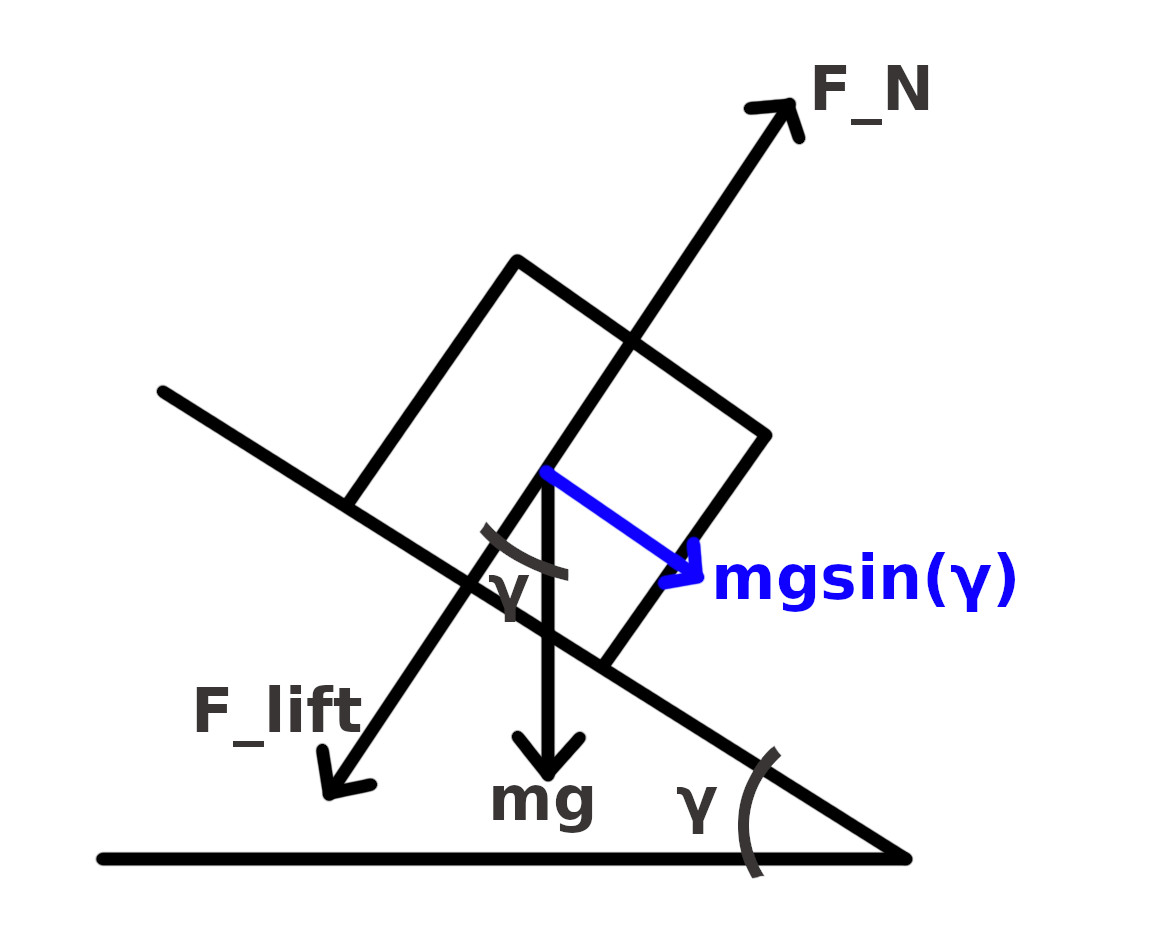
\includegraphics[scale = 0.2]{images/chapter1/equilibriumOnZAxis.jpg}
    \caption{Contribution of mg}
    \label{fig:contribmg}
\end{figure}
\begin{figure}[h!]
    \centering
    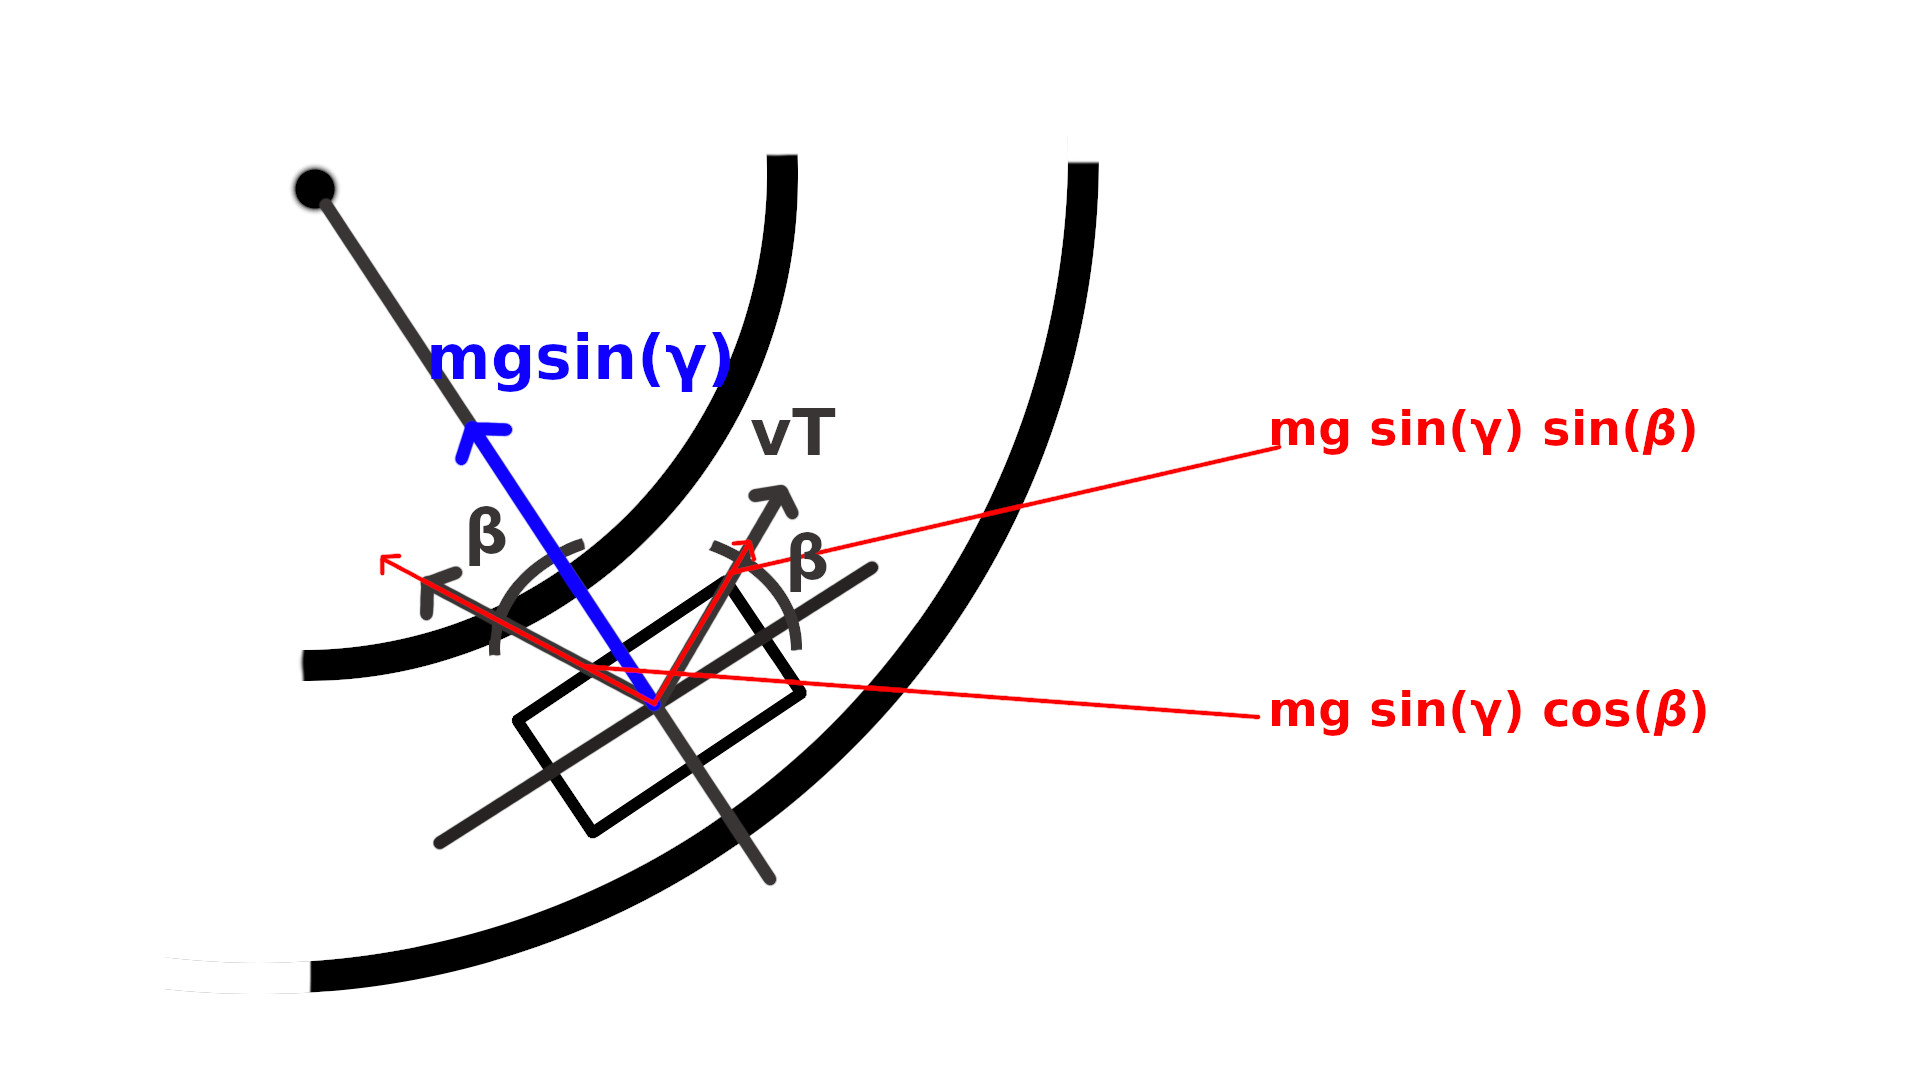
\includegraphics[scale = 0.2]{images/chapter1/basedOnPosition.jpg}
    \caption{Terms affecting the model equations}
    \label{fig:basedonpos}
\end{figure}

In the end, the final equations will be:
\begin{equation}
\begin{aligned}
\\
\dot{x_4} = \frac{F_{xF} cos(x_5-\delta) + F_{xR} cos(x_5) + F_{yF} sin(x_5-\delta) + F_{yR} sin(x_5) -\frac{1}{2} \rho C_x S v^2 \color{red} + mgsin(\gamma) sin(x_5) \color{black}}{m_T} \\
\\
\dot{x_5} = \frac{-F_{xF} sin(x_5-\delta) - F_{xR} sin(x_5) + F_{yF} cos(x_5-\delta) + F_{yR} cos(x_5) - m_T x_4 x_6 \color{red} + mgsin(\gamma) cos(x_5) \color{black}}{m_T x_4} \\
\end{aligned}
\end{equation}


\section{Friction ellipse and wear}
Coming to the conclusion of our model, we took in consideration also the physical relation between longitudinal and lateral forces through the friction ellipse

\begin{equation}
\begin{aligned}
{(\frac{F_x}{F_{x,max}})}^2 + {(\frac{F_y}{F_{y,max}})}^2 = 1
\end{aligned}
\end{equation}

In particular, $F_{x,max}$ and $F_{y,max}$ are respectively the maximum longitudinal and lateral forces, that are are calculated through the Pacejka parameters, being $D + V$ the point of max of the tyre model. Here we recall that: 

\begin{equation}
\begin{aligned}
D_{lat} = F_z (a_1 F_z + a_2) (1 - a_{15} \gamma^2)\\
V_{lat} = a_{11}F_z + a_{12} + (a_{13} F_z + a_{14}) \gamma F_z\\\\
D_{long} = F_z (b_1 F_z + b_2)\\
V_{long} = b_{11}F_z + b_{12} \\\\
\end{aligned}
\end{equation}

Thus as we can see, the maximum longitudinal and lateral forces are functions of the vertical load $F_z$.\\(Note: different parameters are used for longitudinal and lateral Pacejka, in particular $a_i$ is referred to the lateral one while $b_i$ to the longitudinal one).\\\\
In this way the ellipse is defined, but, taking in consideration the wear $h$ the ellipse is scaled. Thus, at the end, $F_{x,max}$ and $F_{y,max}$ are functions of $F_z$ and $h$, specifically:

\begin{equation}
\begin{aligned}
F_{x,max} = (D_{long} + V_{long}) \frac{1}{w_1 h + w_2}\\
F_{y,max} = (D_{lat} + V_{lat}) \frac{1}{w_1 h + w_2}
\end{aligned}
\end{equation}

Where $w_1$ and $w_2$ are parameters opportunely chosen. In this way the more the wear, the more the ellipse is shrunk.\\\\
The ellipse is saying us which is the maximum lateral force wrt the given $F_x$ in input. Thus, finally, the output of the lateral Pacejka is scaled, so to have the peak value ($D_{lat}+V_{lat}$) equal to the value given by the ellipse. To do so, the D value of the Pacejka is directly fed as input to the model through the output of the ellipse.\\Following image tries to clarify the steps detailed so far.

\begin{figure}[h!]
    \centering
    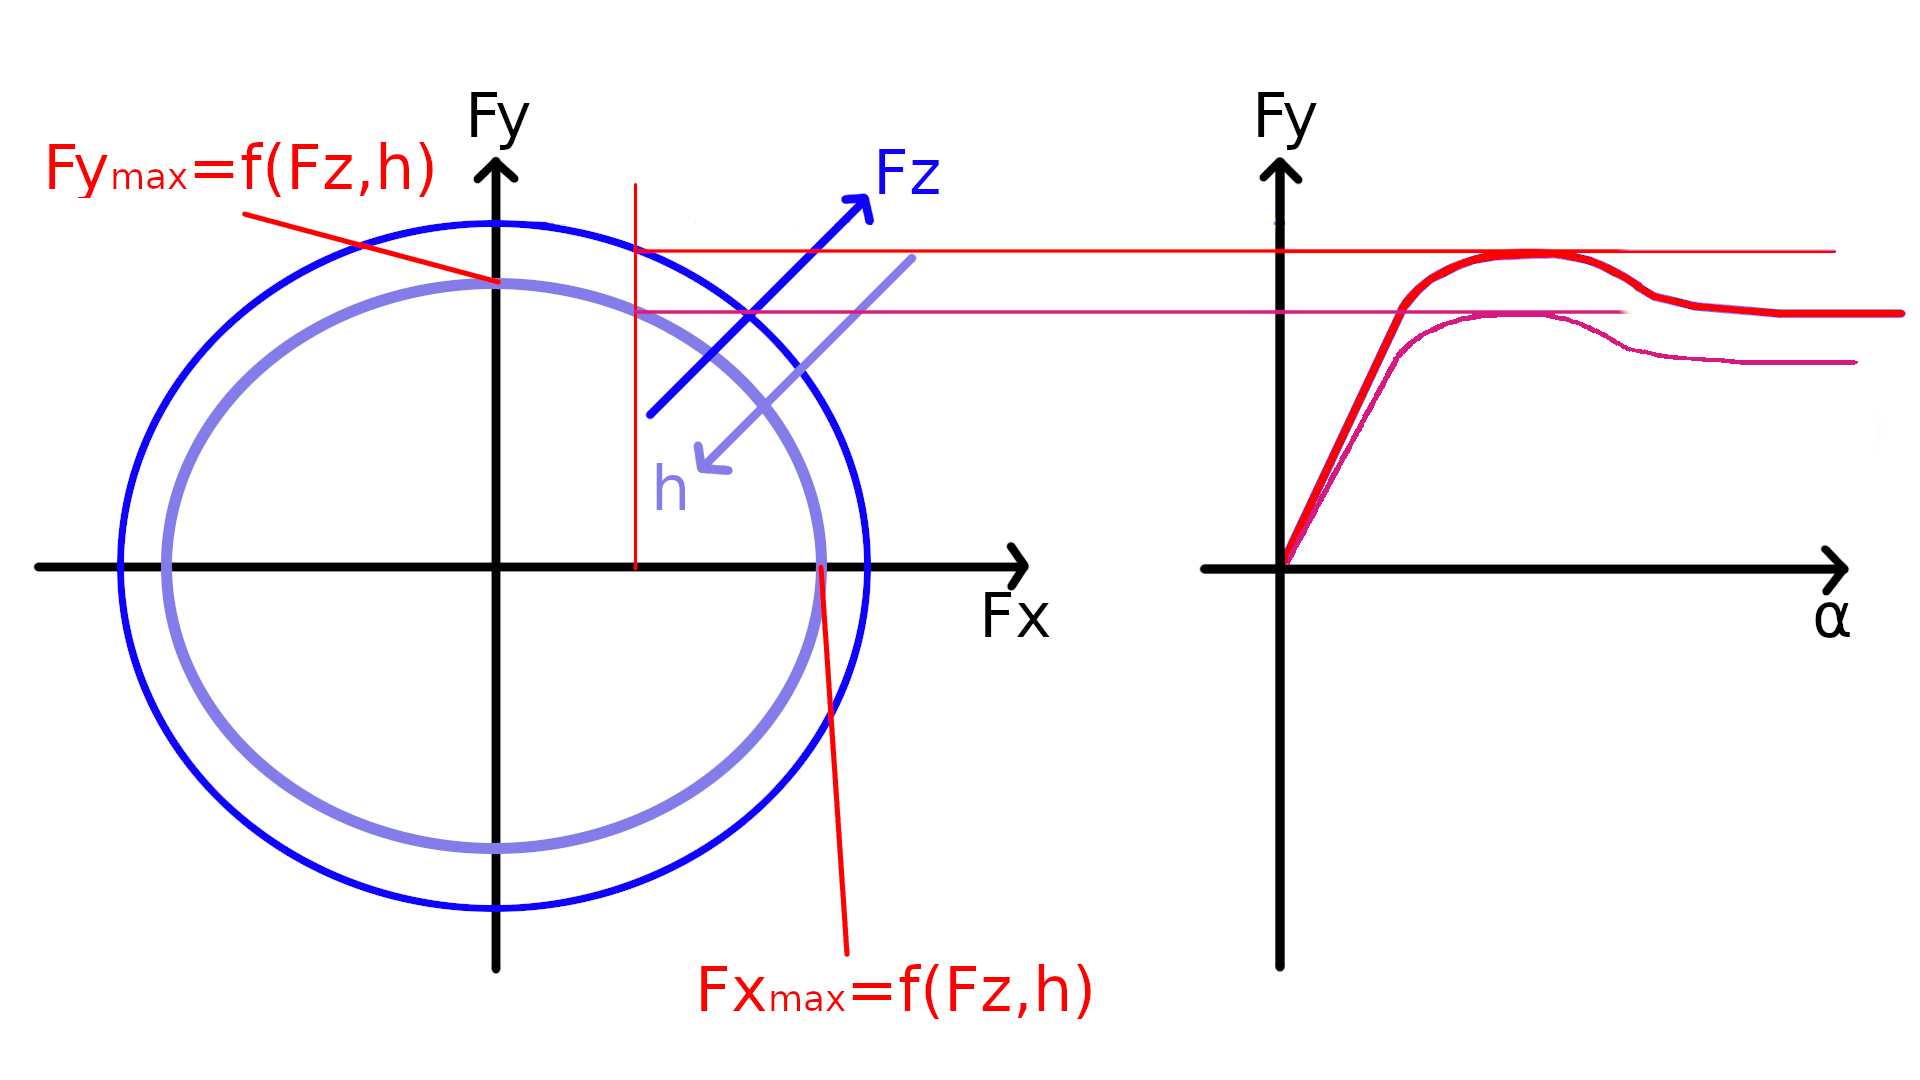
\includegraphics[scale = 0.17]{images/chapter1/ellisse.png}
    \caption{Friction ellipse and wear effects}
    \label{fig:ellisse}
\end{figure}

\newpage

\section{Slipstream}
In our model we also considered the slipstream effect.
The change in the used coefficients is assumed to be different in case of a straight path and in case of a curvature path. We assume for simplicity that along a straight path the two vehicles are perfectly aligned (thus having 0 offset) while along curvature paths the mean offset is considered different from 0. The changes in the drag force or in the lift force that occur while the vehicle is undergoing slipstream assume that the ego vehicle is really close to the following vehicle: the distance is around $0.5*L$ where $L$ is the rear-front wheeel distance. In particular for a:
\begin{itemize}
 \item straight path: the drag force decrease is of 15\% while the lift force decrease is of 30\% 
 \item curvature path: the drag force decrease is of 15\% while the lift force remains the same 
 \end{itemize}
 All the used coefficients can be found in the Appendix A. 

\section{Simulations}
Different simulations have been run to validate qualitatively the presented model and to highlight its most relevant features. Among the others, 5 simulations are considered to be the most representative and are shown in the following. For each simulation only the most relevant graphs have been shown. For a complete overview of the simulations we refer to this link \url{https://github.com/cvalore/simulations\_logs} where it is possible to find the logs and all graphs related to these simulations.
Note: In all the simulations the input $\delta$ is reported, that is the wheel-angle although we directly fed the steer-angle. They can be reciprocally easy calculated knowing that the steering ratio $\frac{steer\_angle}{wheel\_angle} = 10$.


\subsection{Simulation 1 - Non-accelerating straight path}
In this preliminary simulation the aim was to test the correctness of the various figures of merit in a flying start situation with an initial velocity of $20[m/s]$ and nothing else. Provided inputs are $F_x = 0 [N]$, $\delta = 0 [rad]$, simulation time = $30 [s]$. Banking is not considered. 
\\Although not very significant, this test guarantees that all the internal forces are working correctly. Indeed, the decreasing of the acceleration and velocity due to the aerodynamic force can be seen in the figure \ref{fig:sim1_1}. All the other figures are not useful, since all angles, lateral forces, power and mass decreasing factor are zero; also the trajectory is not reported since it is simply a straight line. \\

\begin{figure}[h!]
    \centering
    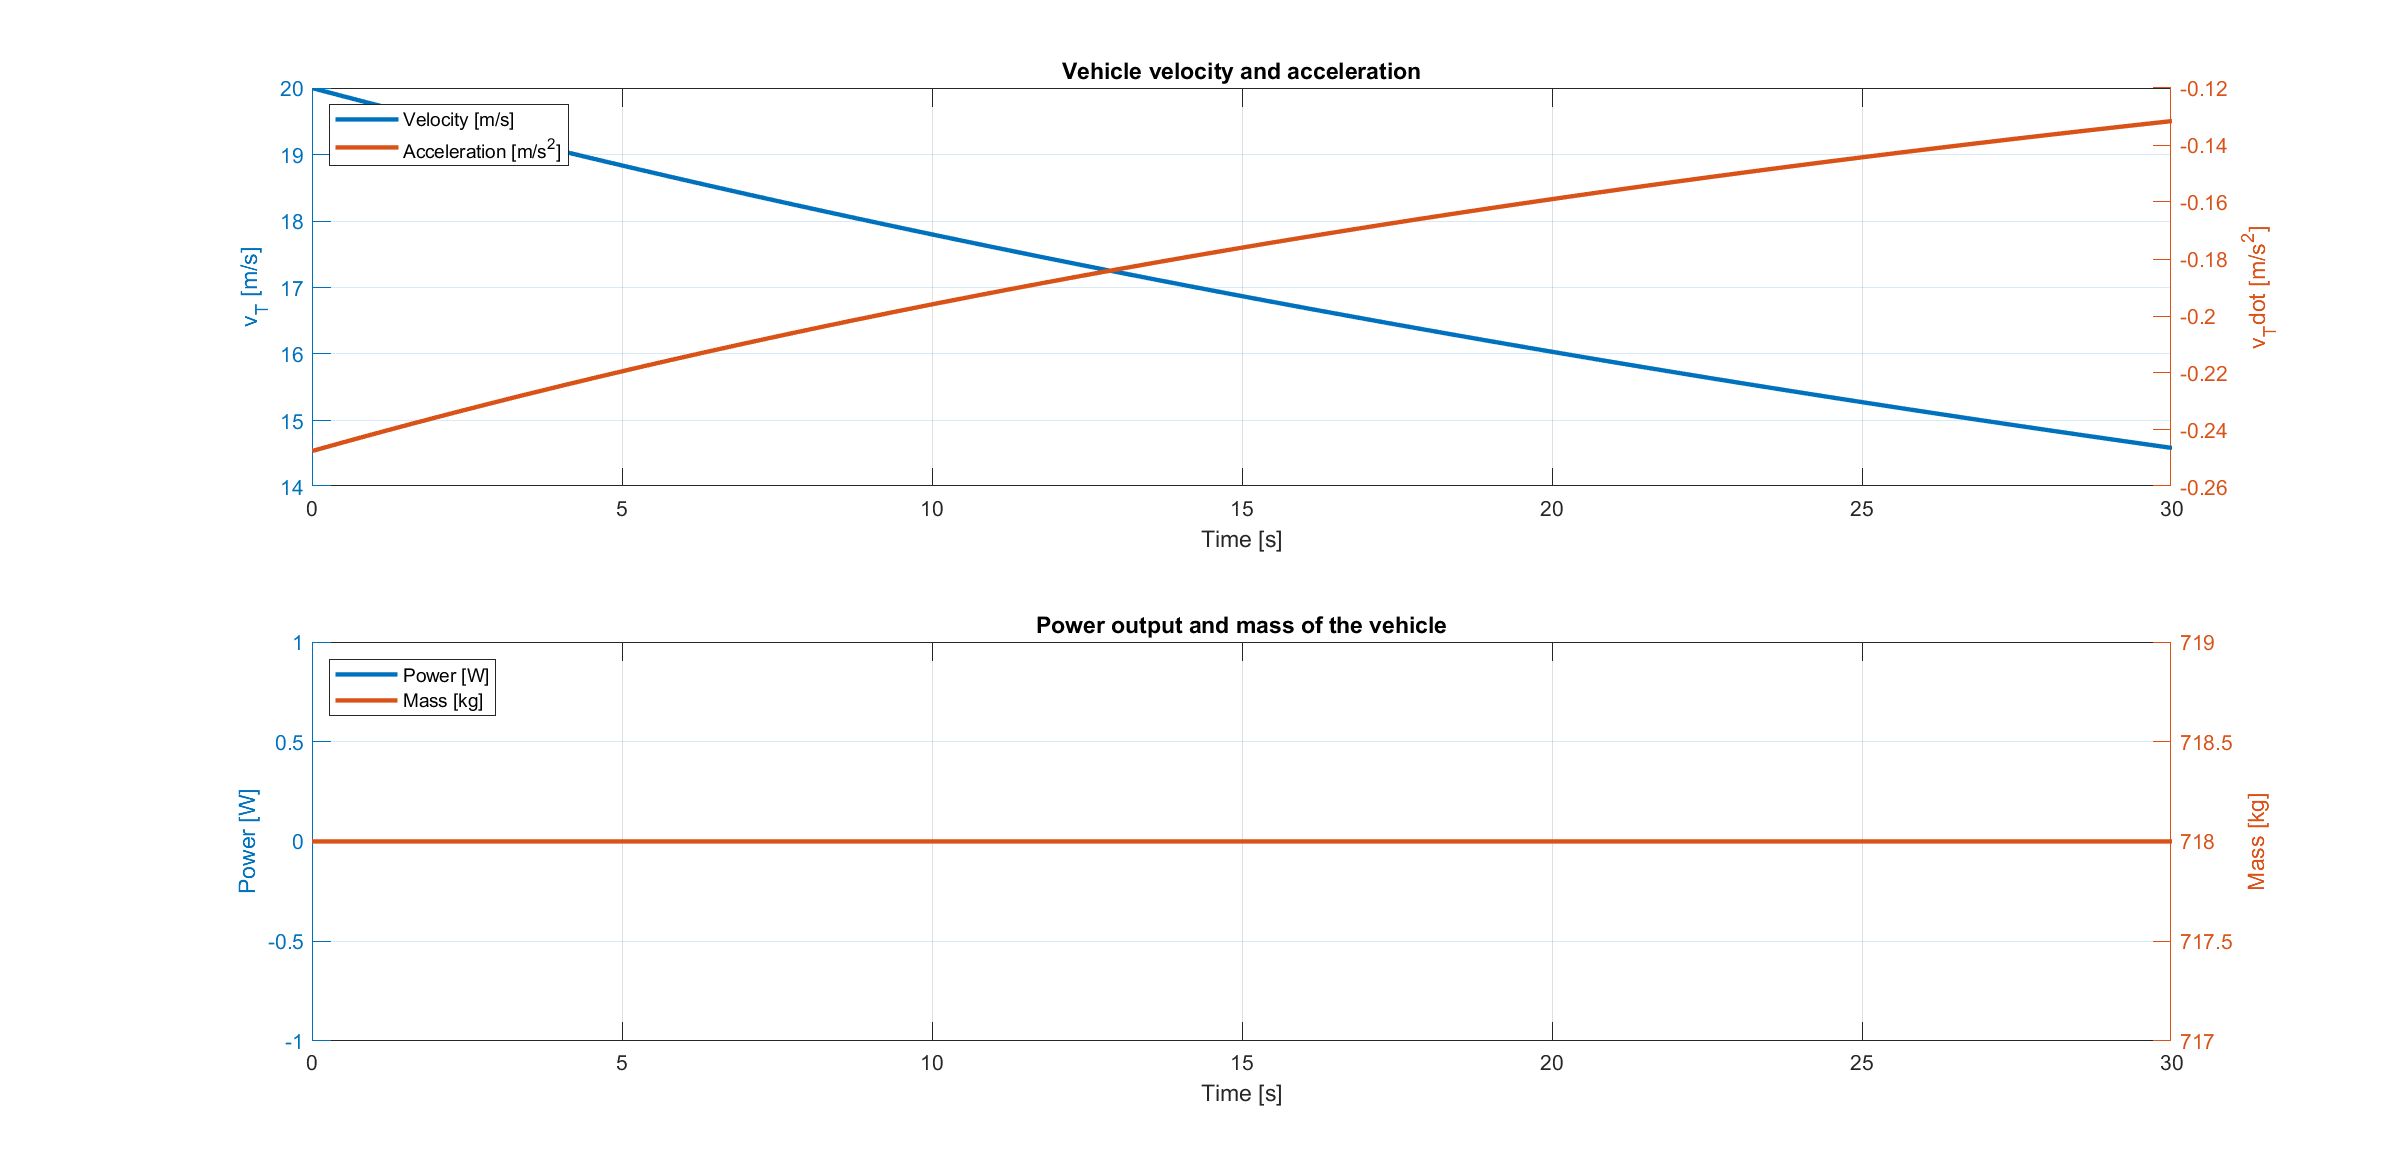
\includegraphics[width=\linewidth]{images/chapter1/simulations/sim1_vel-power.png}
    \caption{Simulation 1 - velocity, acceleration, power and mass figure}
    \label{fig:sim1_1}
\end{figure}

\subsection{Simulation 2 - Accelerating straight path}
In this preliminary simulation the aim was to test the correctness of the various figures of merit in a situation in which the initial velocity of the vehicle is $0[m/s]$ and there is a constant acceleration. Provided inputs are $F_x = 1000 [N]$, $\delta = 0 [rad]$, simulation time = $30 [s]$. Banking is not considered.
\\Also in this case not every simulation result is shown, since angles and trajectory are, as before, respectively zero and a straight line. The velocity and acceleration figure is shown and it is consistent with the given simulation data; the first one is increasing since there is a constant force applied over all the time interval that makes the acceleration always positive, the second one is decreasing since the applied force is not changing over the time and the aerodynamic force is increasing with the square of the velocity. The figures reported, figures \ref{fig:sim2_1} and \ref{fig:sim2_2} are showing as the tyres wear is increasing with time and how the power is effecting the mass of the vehicle (actually the mass of the fuel) that is decreasing.\\ 
\begin{figure}[h!]
    \centering
    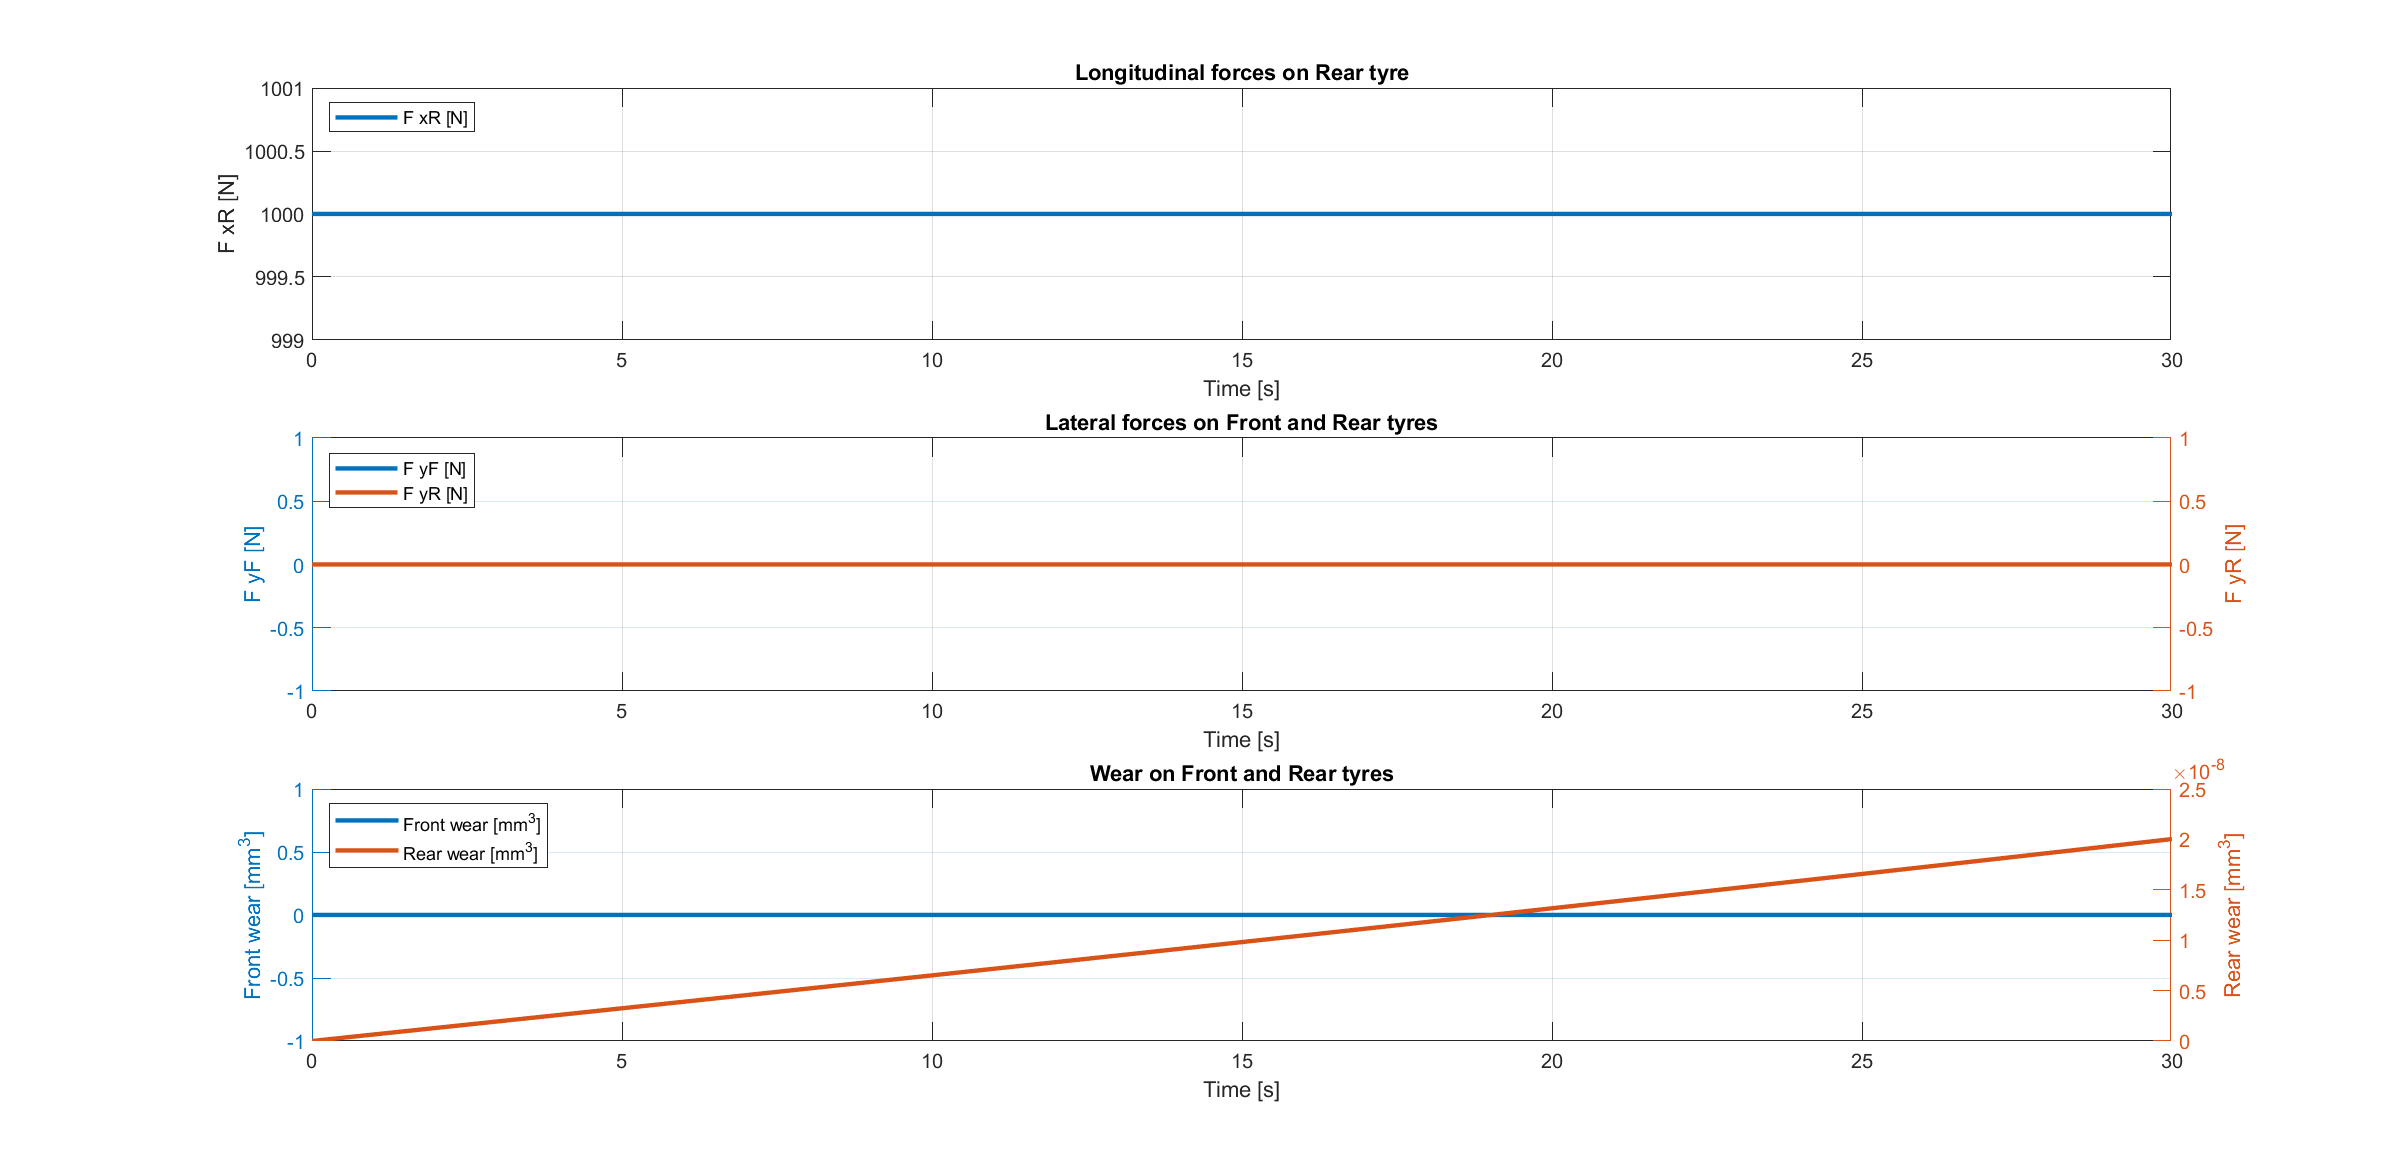
\includegraphics[width=\linewidth]{images/chapter1/simulations/sim2_force-wear.png}
    \caption{Simulation 2 - forces and tyres wear figure}
    \label{fig:sim2_1}
\end{figure}
\begin{figure}[h!]
    \centering
    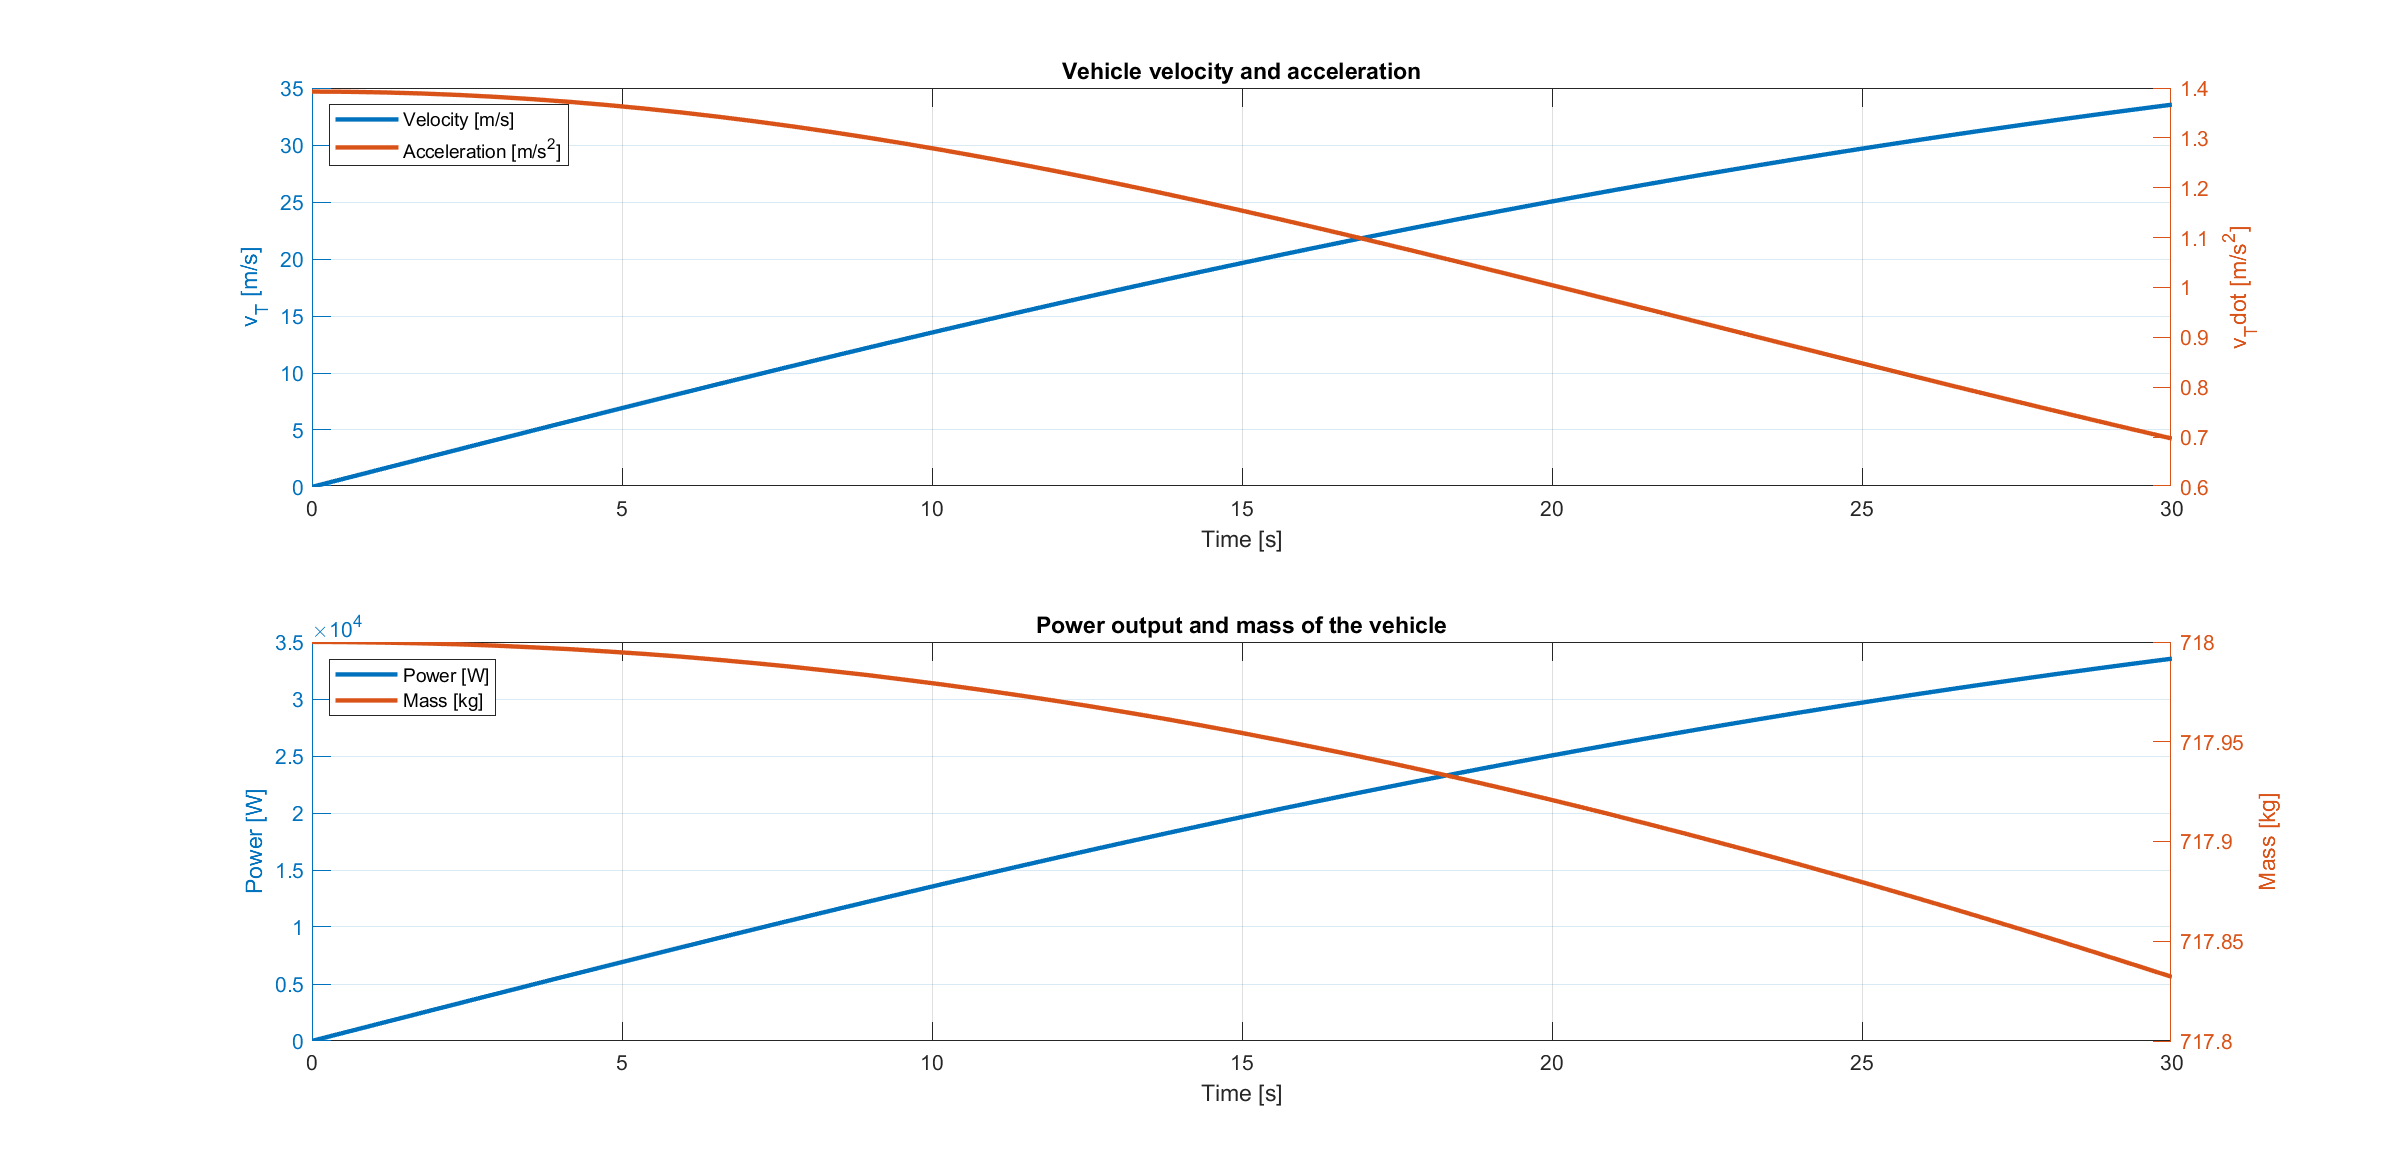
\includegraphics[width=\linewidth]{images/chapter1/simulations/sim2_vel-power.png}
    \caption{Simulation 2 - velocity, acceleration, power and mass figure}
    \label{fig:sim2_2}
\end{figure}

\subsection{Simulation 3 - Accelerating straight path on a banked road}
In this simulation the aim was to test the correctness of the various figures of merit when the ego vehicle traverses a banked road. Provided inputs are: $F_x = 500 [N]$, $\delta = 0 [rad]$, simulation time = $50 [s]$. 

\begin{figure}[h!]
    \centering
    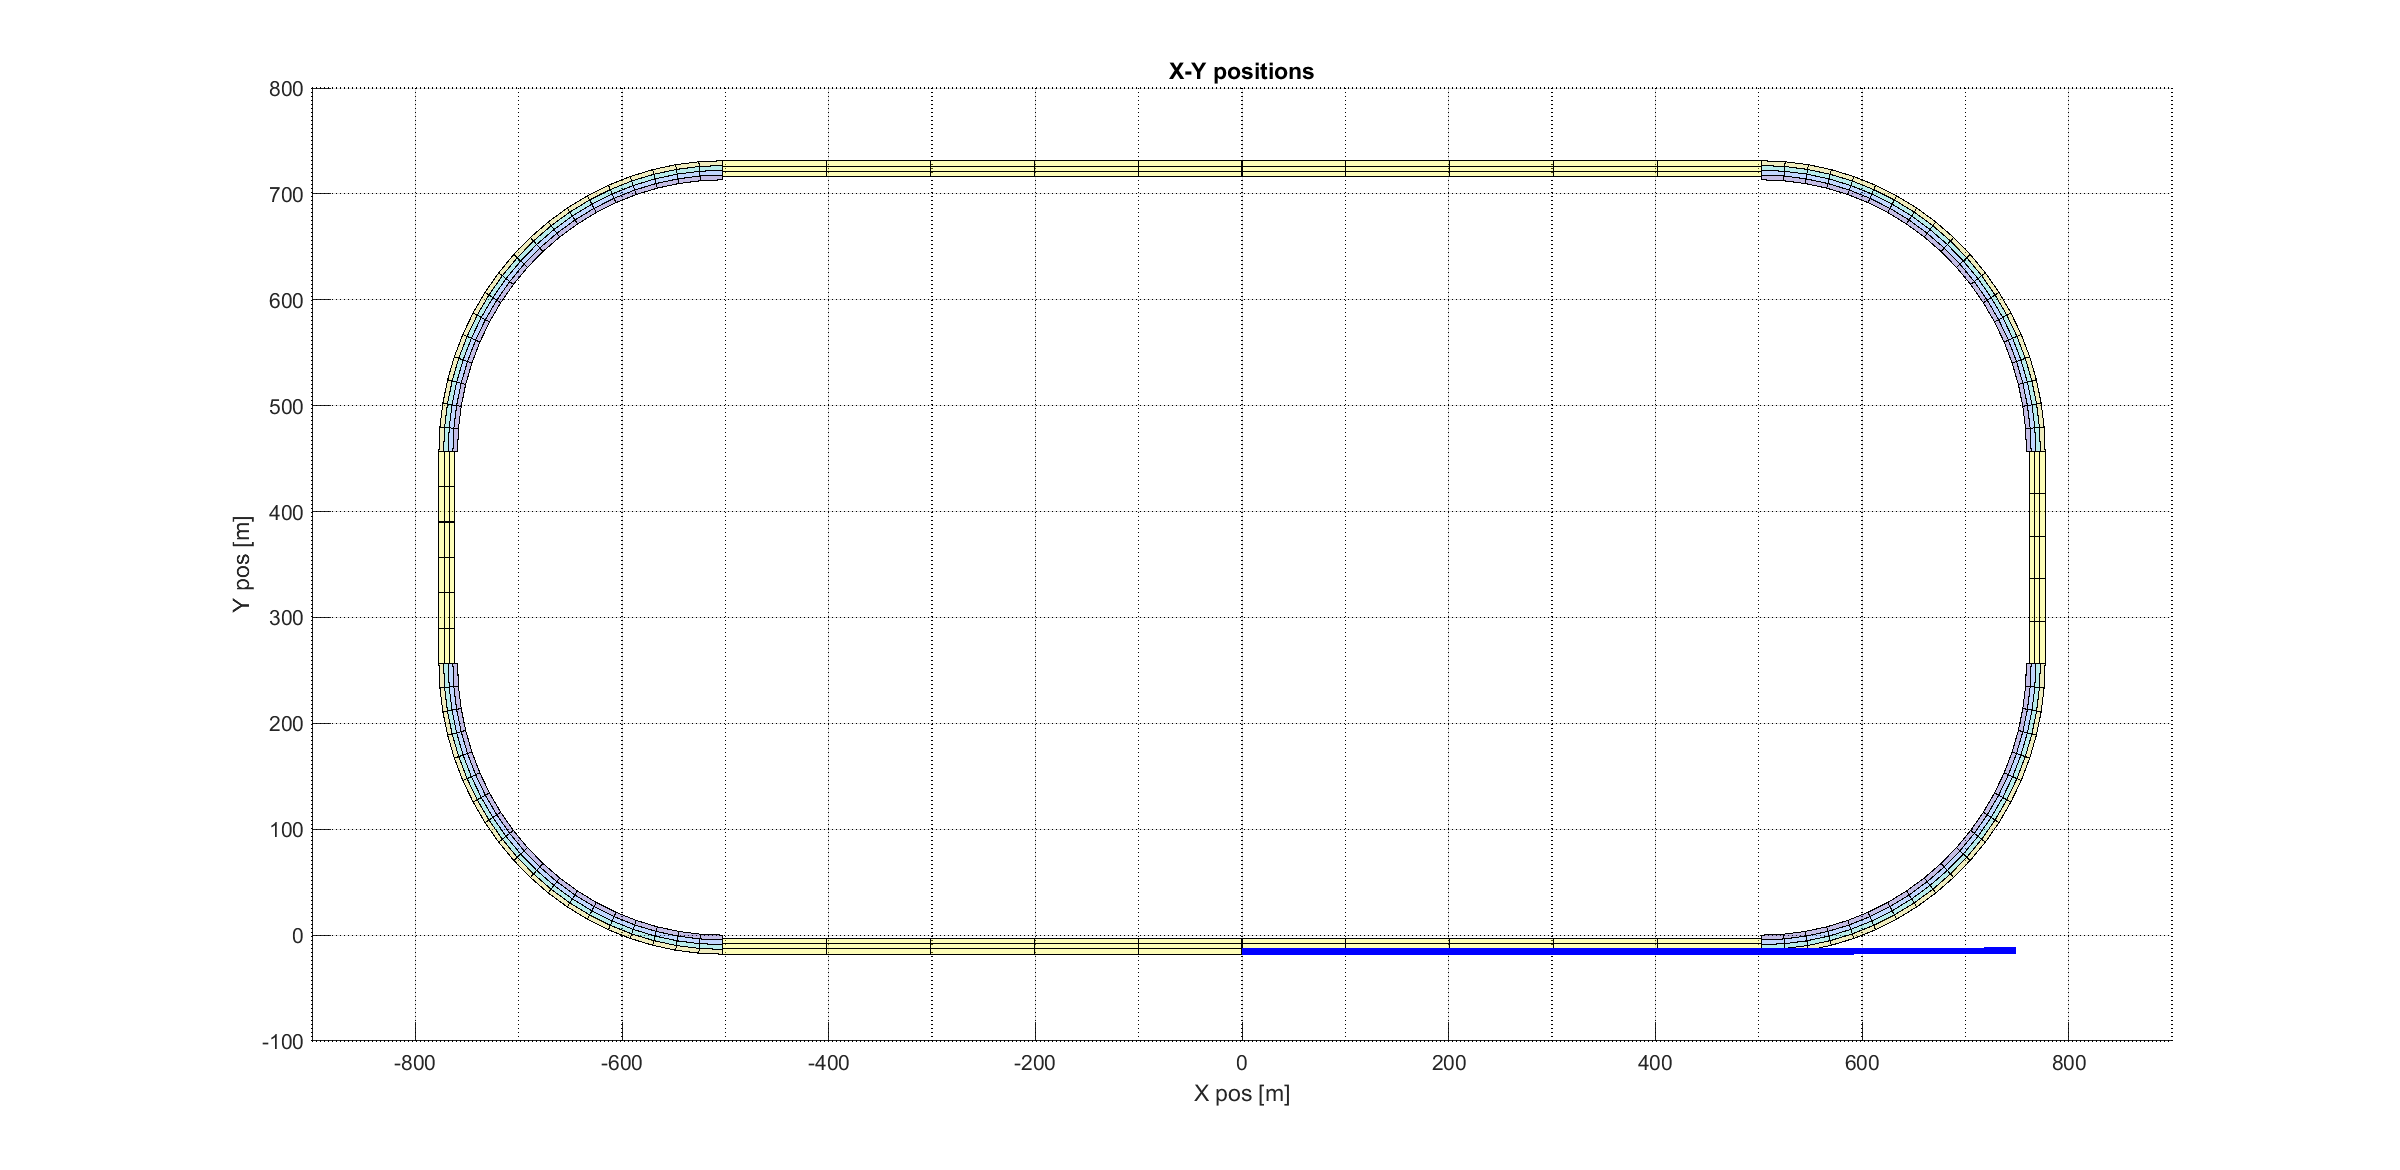
\includegraphics[width=\linewidth]{images/chapter1/simulations/sim3_trajectory.png}
    \caption{Simulation 3 - trajectory of the vehicle on the banked road}
    \label{fig:sim3_1}
\end{figure}

\begin{figure}[h!]
    \centering
    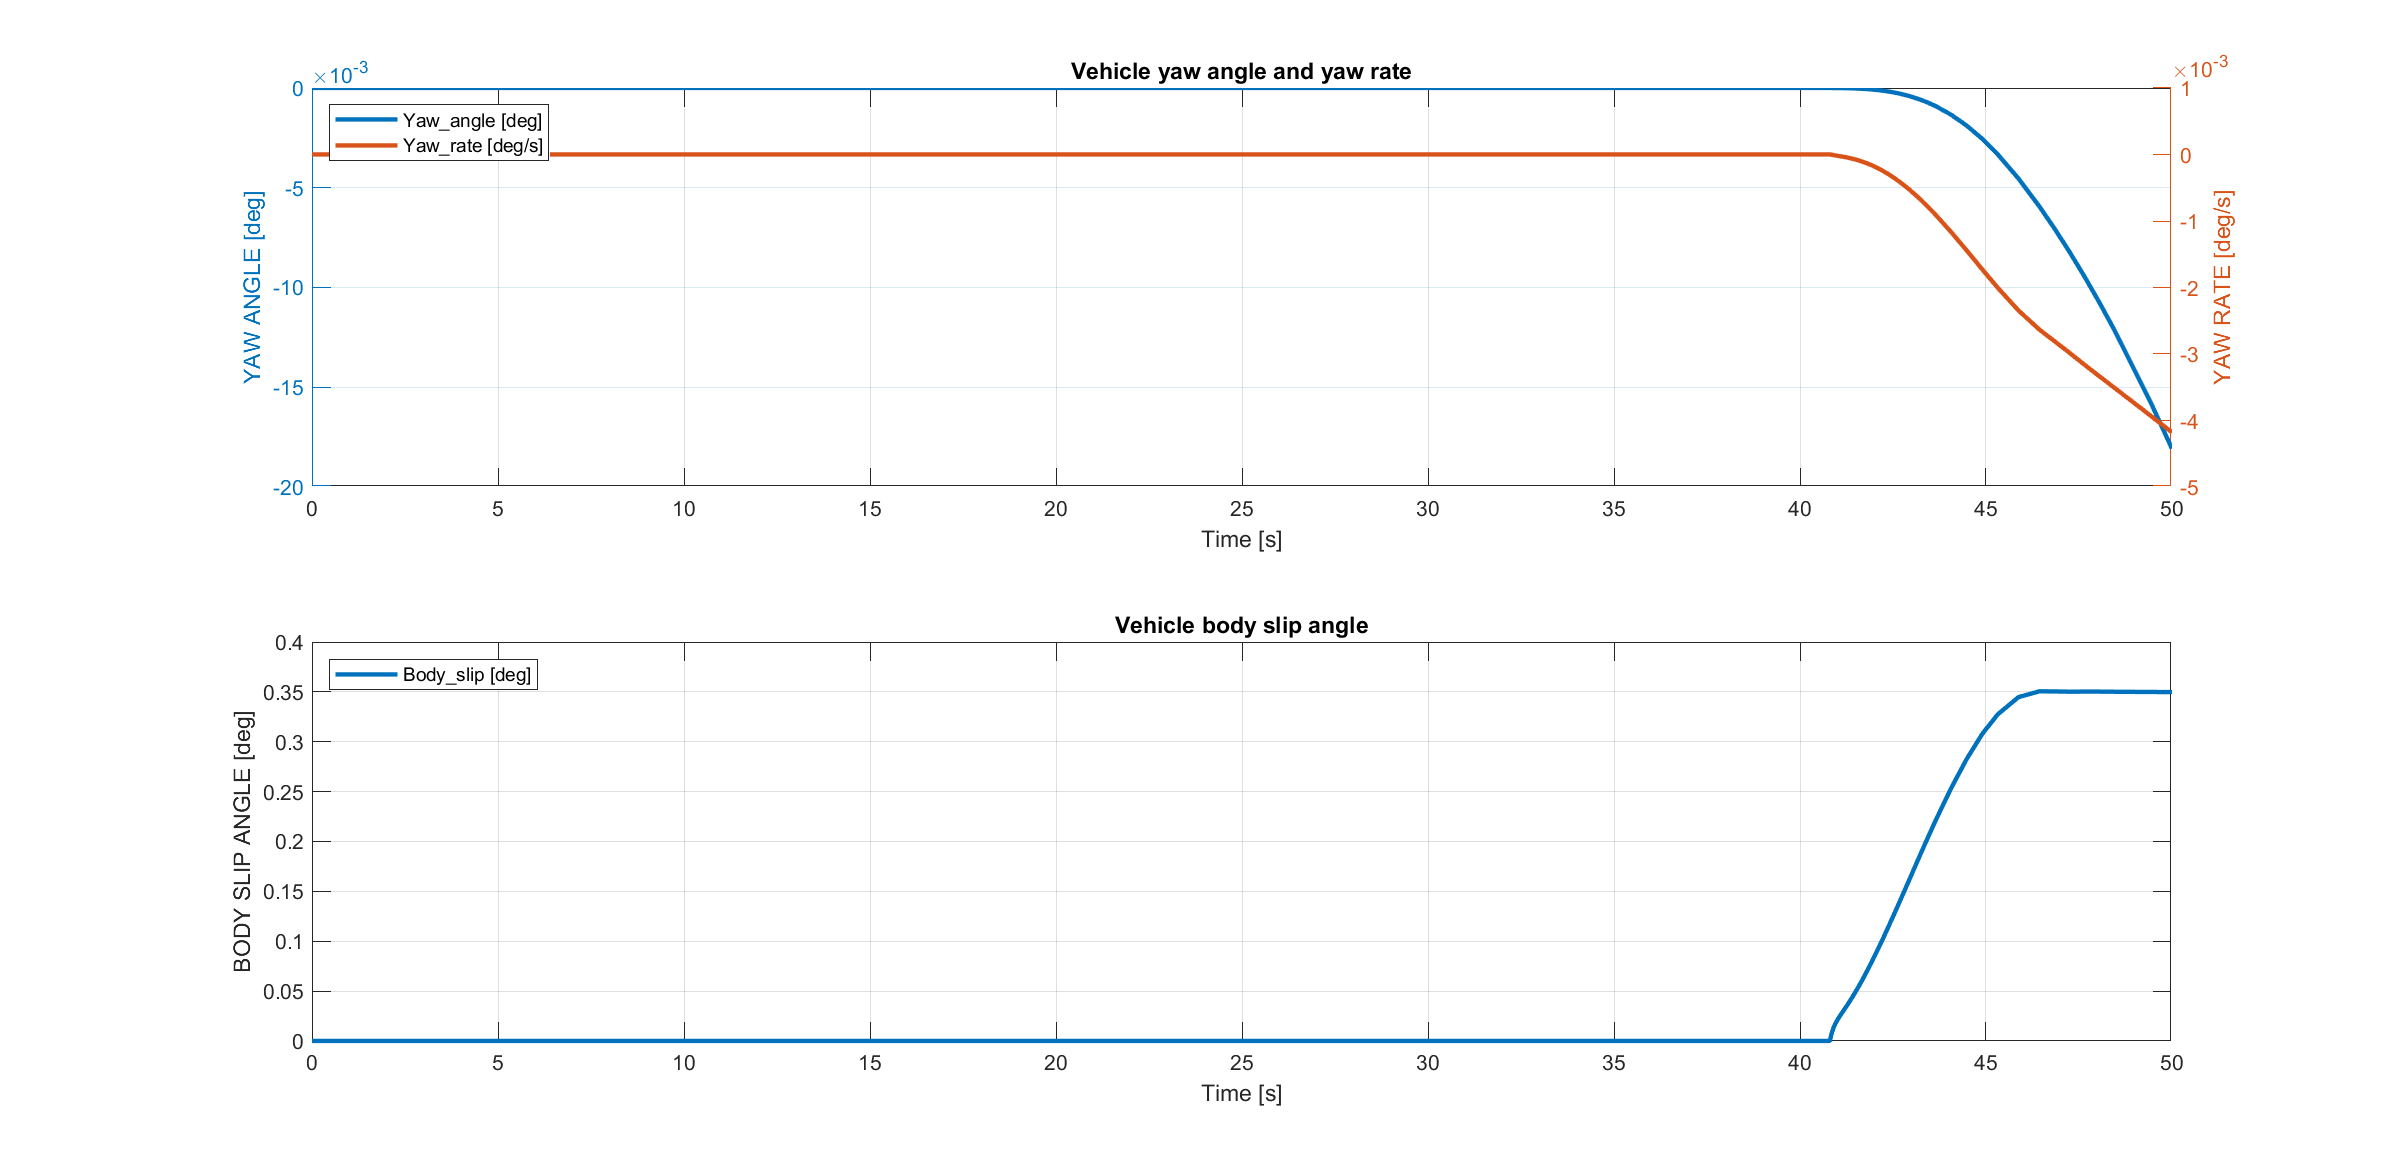
\includegraphics[width=\linewidth]{images/chapter1/simulations/sim3_angles.png}
    \caption{Simulation 3 - angles figure}
    \label{fig:sim3_2}
\end{figure}

\begin{figure}[h!]
    \centering
    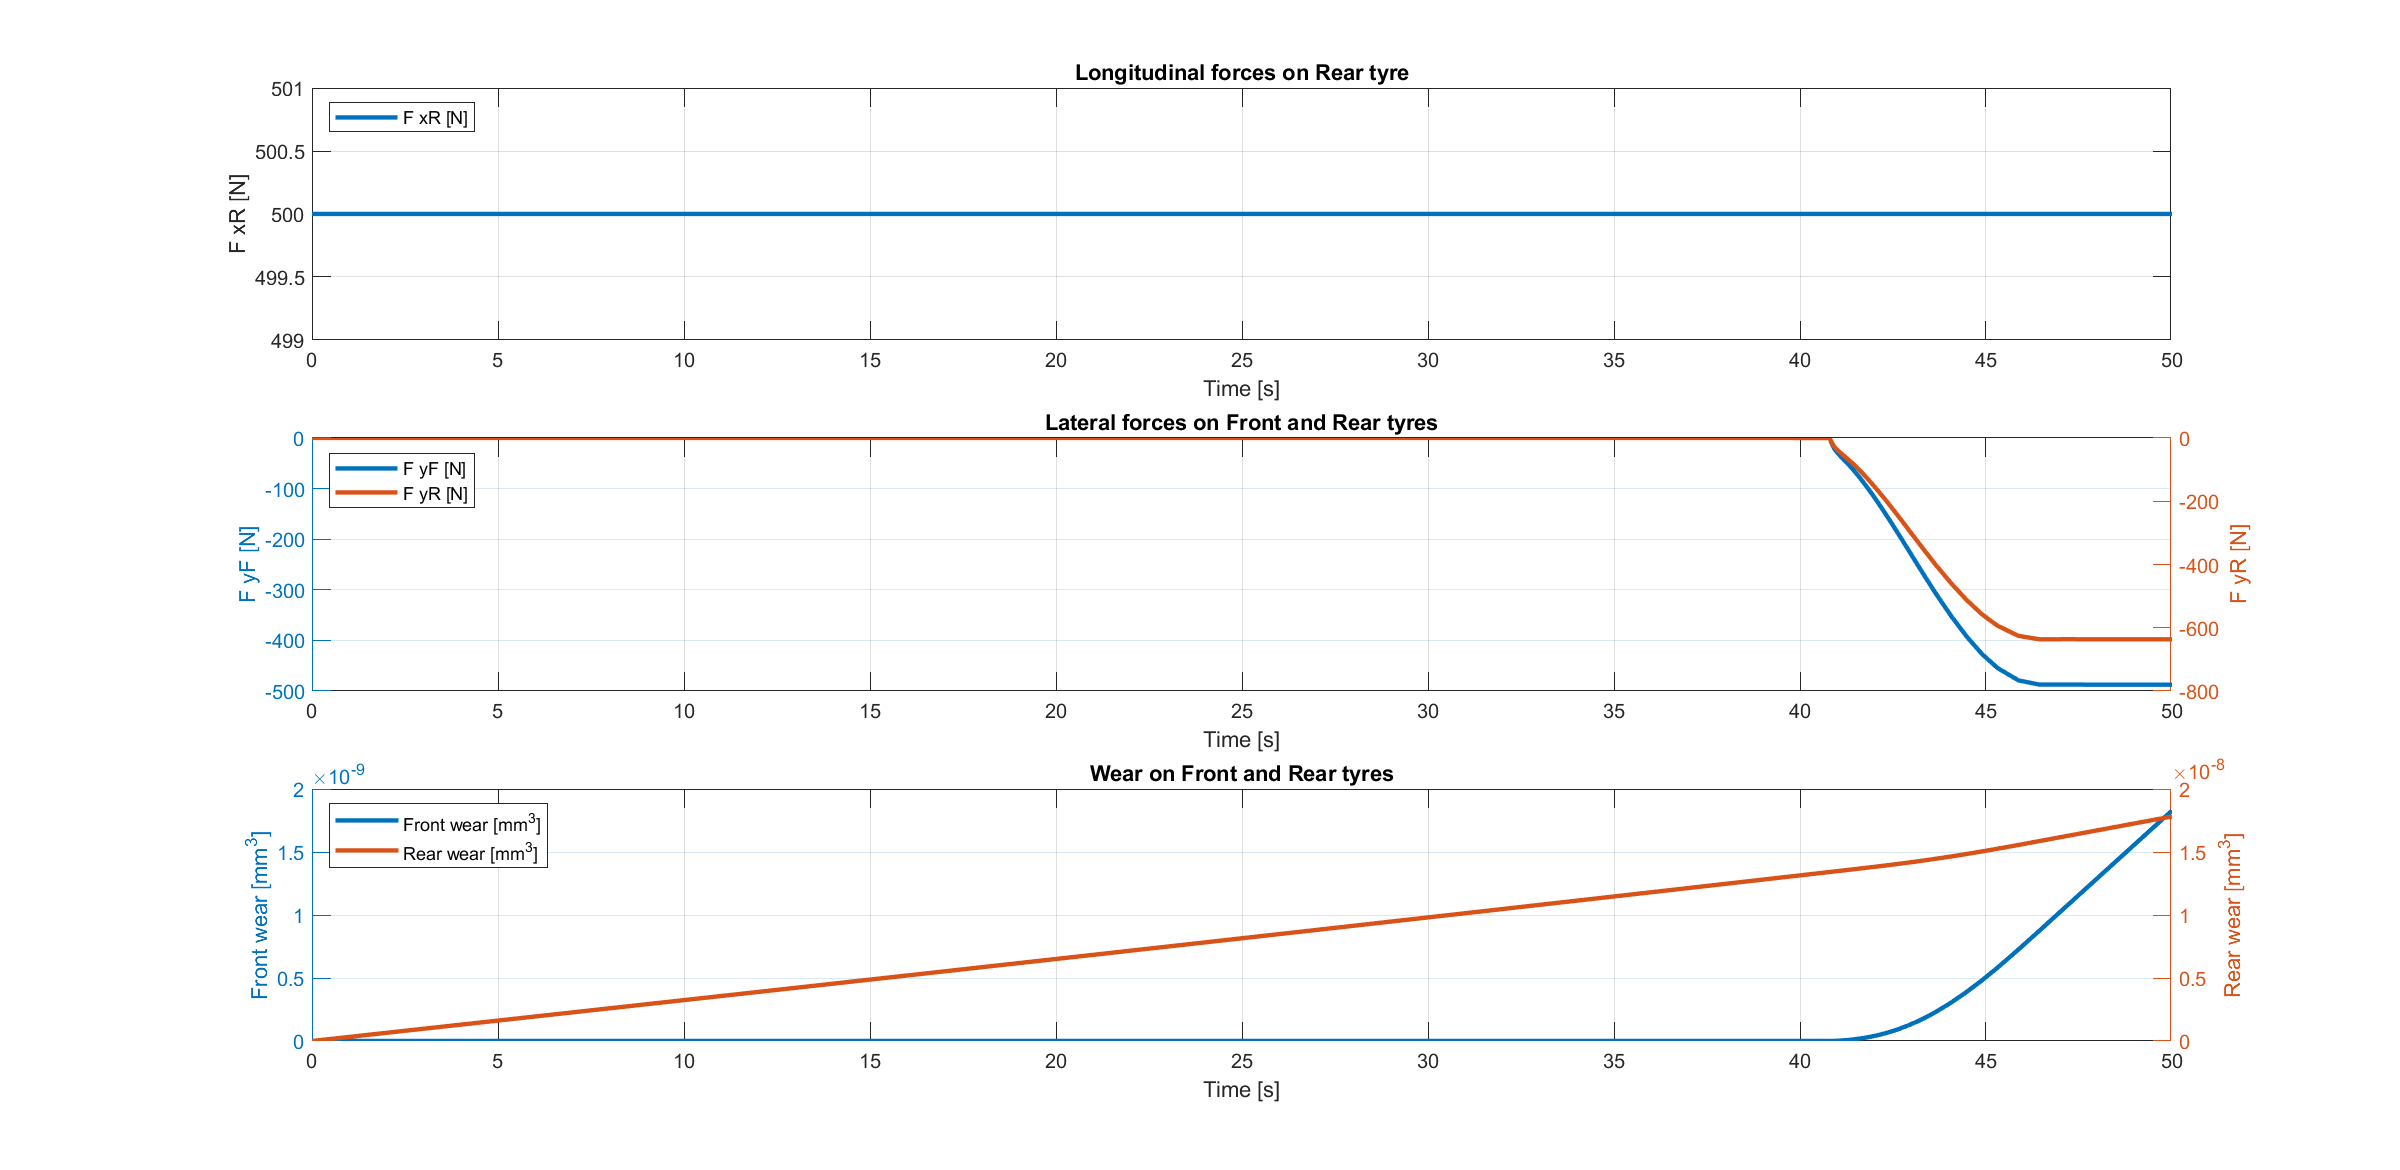
\includegraphics[width=\linewidth]{images/chapter1/simulations/sim3_force-wear.png}
    \caption{Simulation 3 - forces and tyres wear figure}
    \label{fig:sim3_3}
\end{figure}

\begin{figure}[h!]
    \centering
    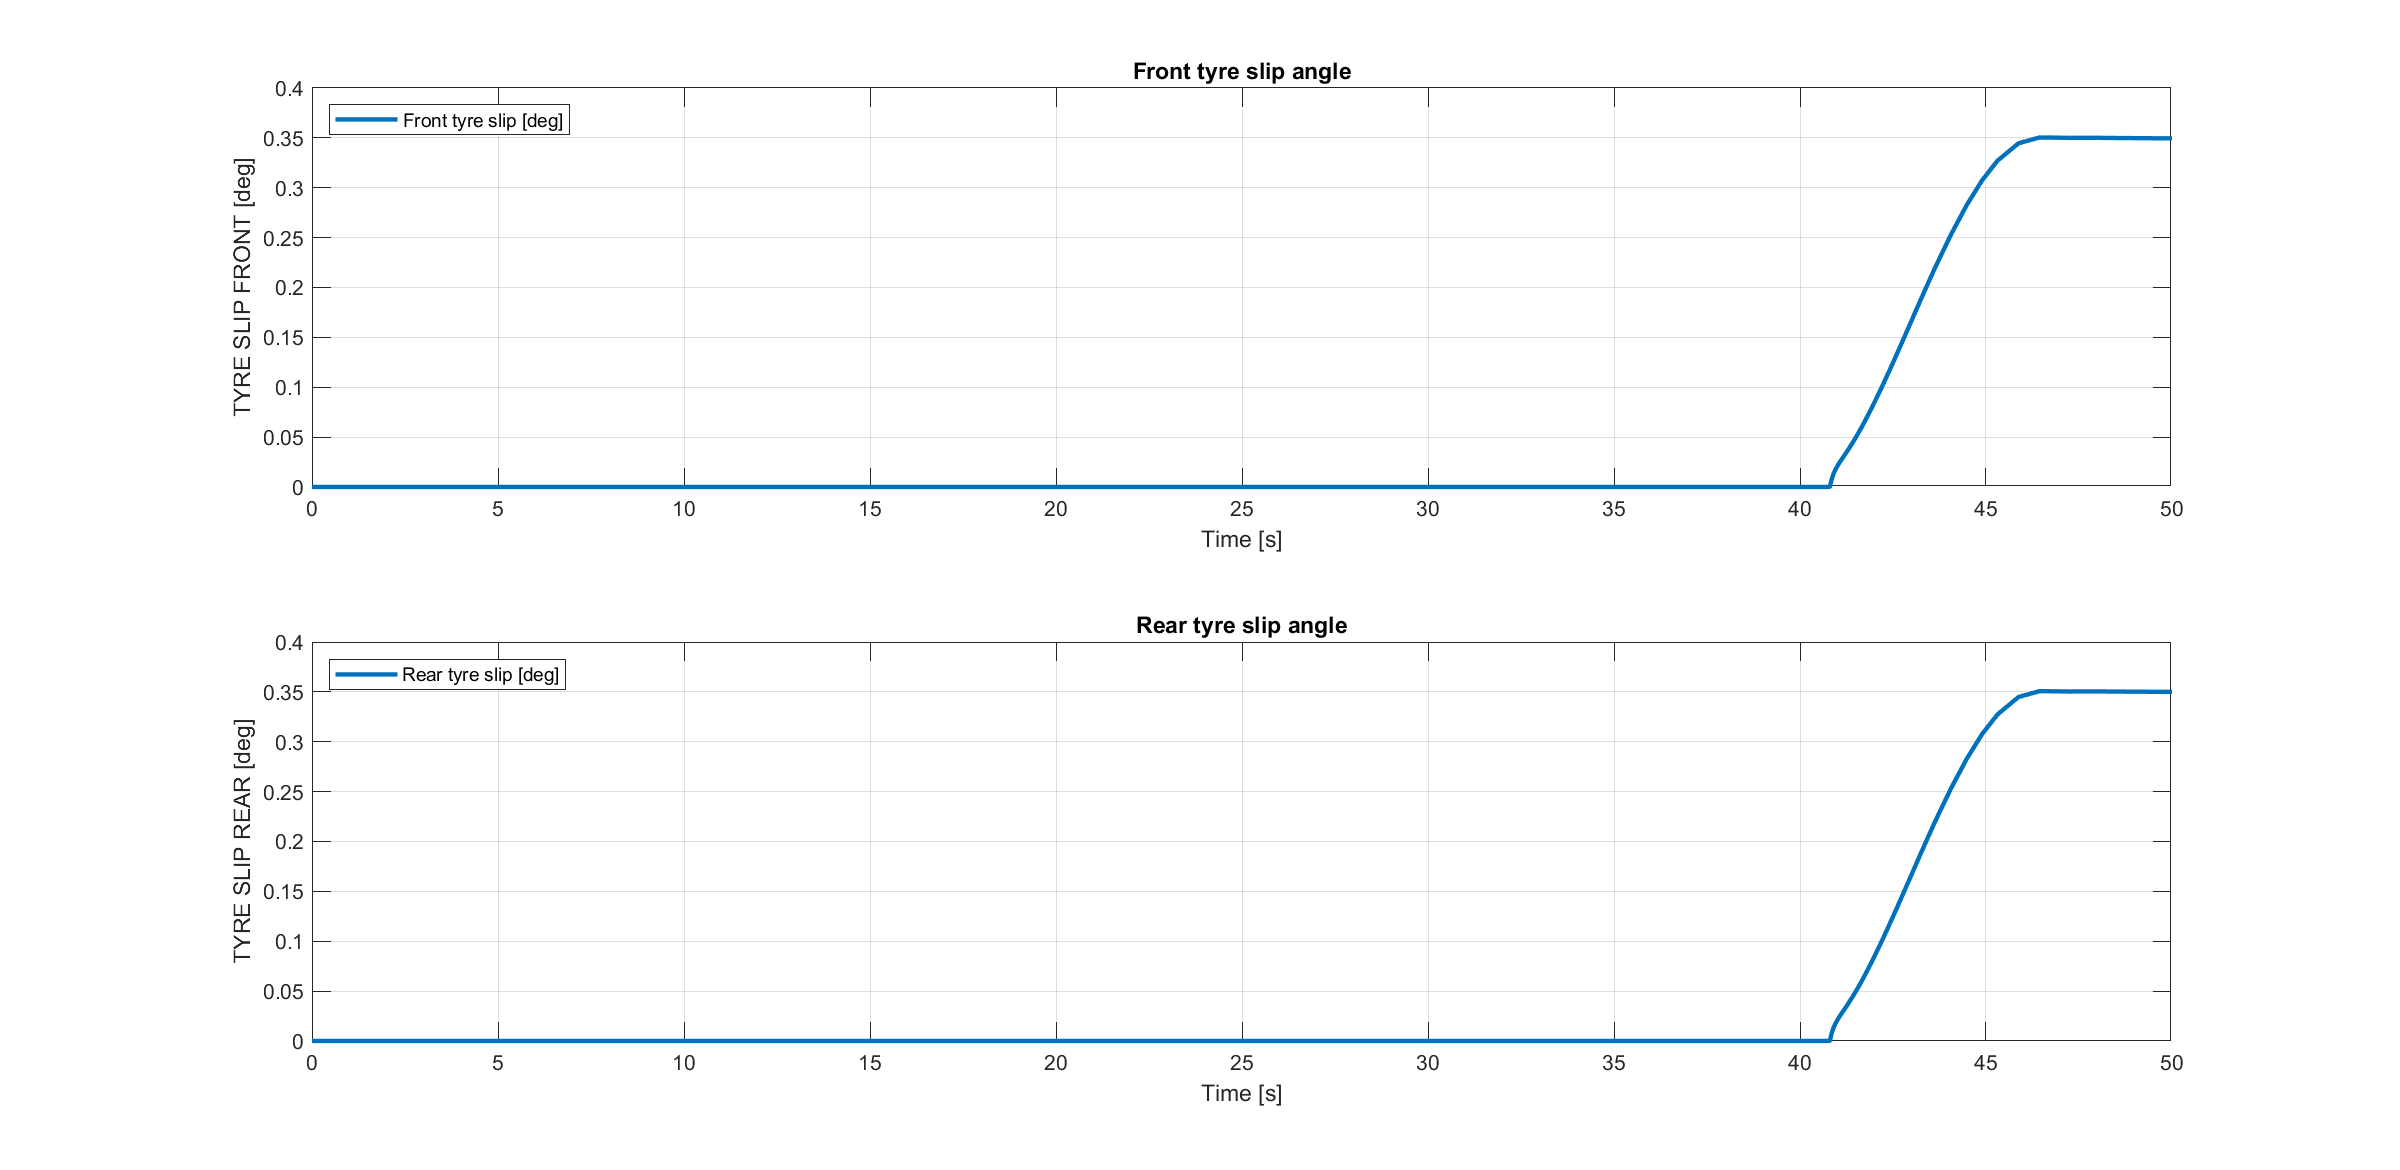
\includegraphics[width=\linewidth]{images/chapter1/simulations/sim3_slips.png}
    \caption{Simulation 3 - tyre slips figure}
    \label{fig:sim3_4}
\end{figure}

As can be seen, when the ego vehicle starts traversing a banked road about at time 40[s], slip angles, lateral forces and other related figures of merit assume non-zero values. This is clearly consistent with the model dynamics that also takes into account the projection of the vertical load on the inclined road.\\


\subsection{Simulation 4 - Accelerating-Breaking straight path}
In this simulation the aim was to show how the considered figures of merit change when the car is moving on a straight line with positive acceleration and then a braking force is applied to reduce its speed. Provided inputs are: $F_x$ in the form of a step function with $F_x = 1250 [N]$ for $15[s]$, $F_x = -700 [N]$ for the following $15[s]$, $\delta = 0 [rad]$, simulation time = $30 [s]$. Banking is not considered.

\begin{figure}[h!]
    \centering
    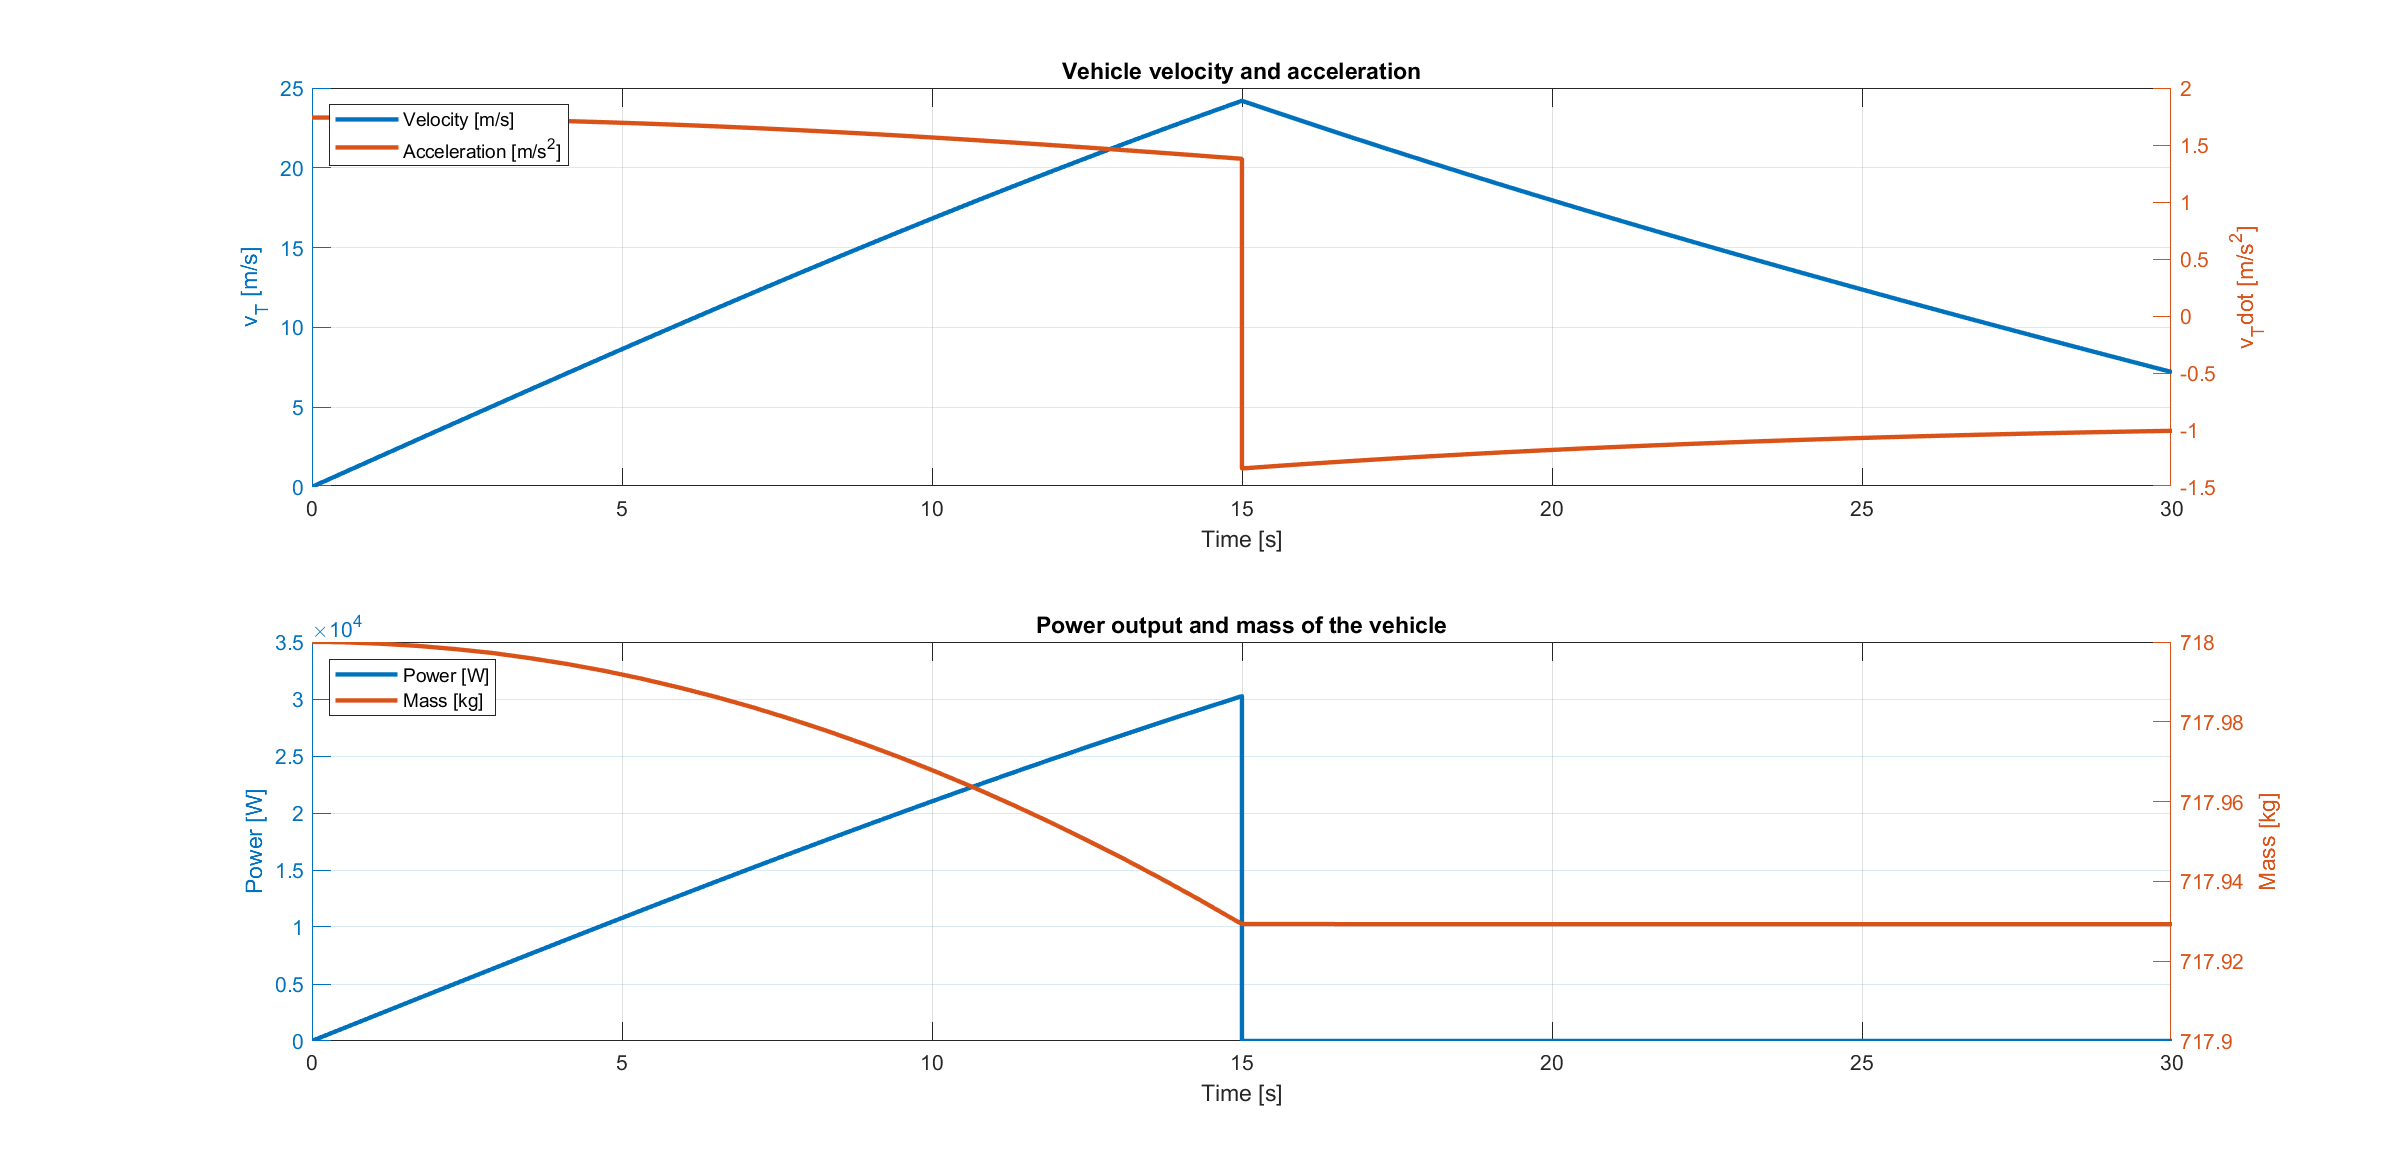
\includegraphics[width=\linewidth]{images/chapter1/simulations/sim4_vel-power.png}
    \caption{Simulation 4 - velocity, acceleration, power and mass figure}
    \label{fig:sim4_1}
\end{figure}

\begin{figure}[h!]
    \centering
    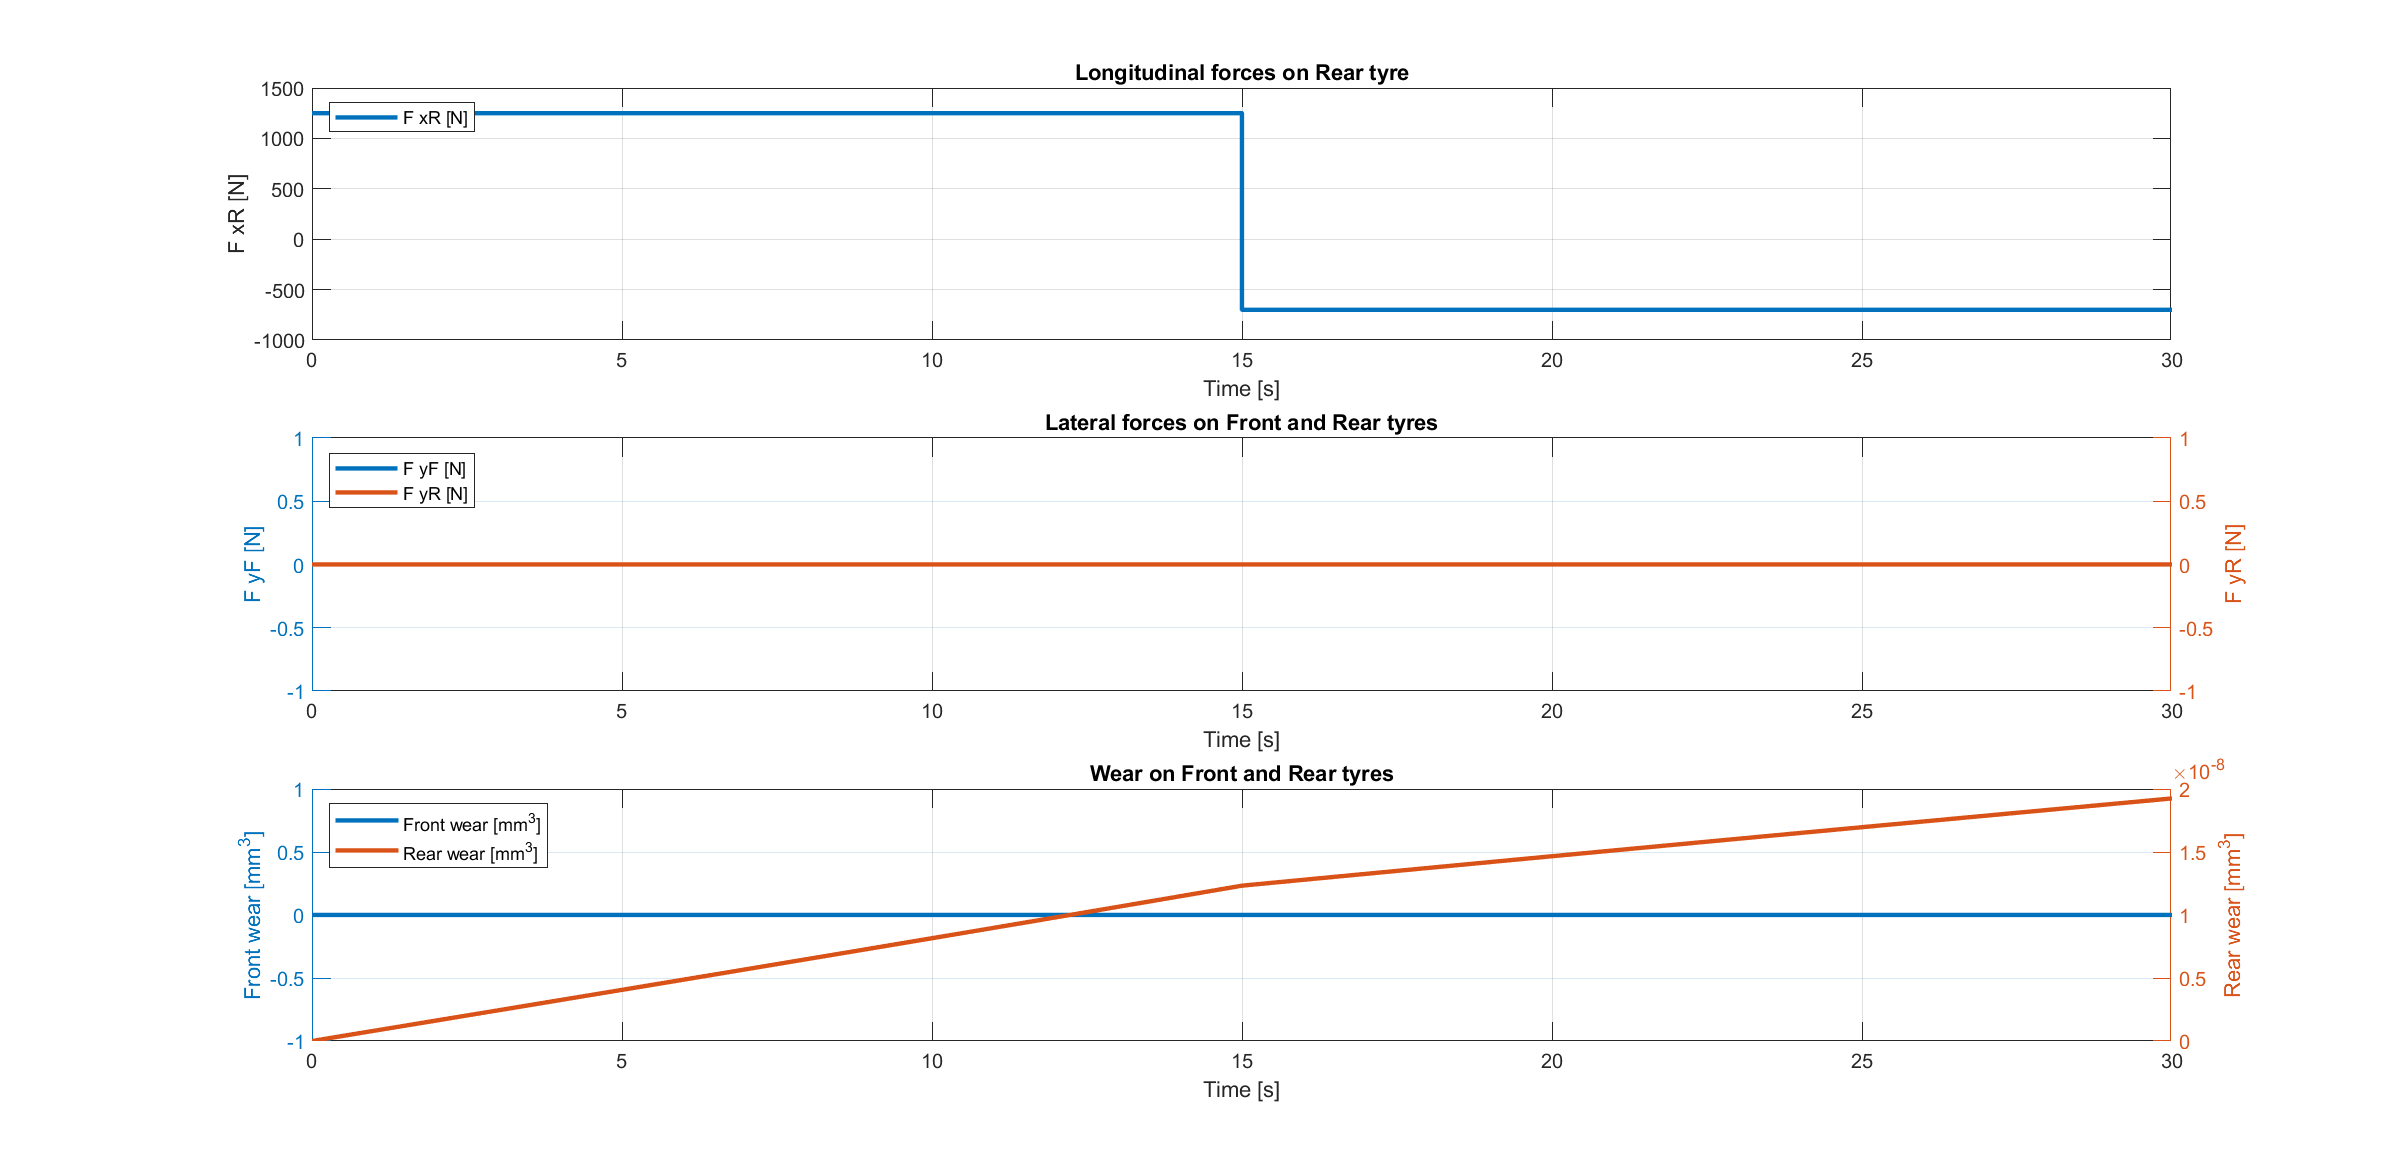
\includegraphics[width=\linewidth]{images/chapter1/simulations/sim4_force-wear.png}
    \caption{Simulation 4 - forces and tyres wear figure}
    \label{fig:sim4_2}
\end{figure}

In this simulation the images related to the figures of merit such as trajectory, slip angle and yaw angles are omitted because always keep a zero value. The shown images are consistent with the vehicle dynamics: as we can see the velocity increases as far as $F_x$ is positive and starts decreasing in the second half of the simulation when $F_x$ holds a negative value. Another important aspect that can be highlighted is the model of the fuel tank that is coherent with the shown results: when the input force $F_x$ has negative values the power produced by the vehicle is considered null as well as the fuel consumption.\\

\subsection{Simulation 5 - Constant steer and increasing velocity path}
The aim of simulation 5 was to test the correctness of the various figures of merit in a "circle trajectory" situation with increasing velocity. The car starts with an initial speed of $0[m/s]$ and then constantly accelerates and steers to the left. Provided inputs are $F_x = 1500 [N]$, $\delta = 0 [rad]$ for the first $0.5[s]$ and then constantly increases up to about $0.03 [rad]$, simulation time = $45 [s]$.
\\In this case the shown figures represent the trajectory, the angles and the lateral forces. As can be seen, the yaw angle constantly increases, since the vehicle is constantly turning, and up to a certain time point also the yaw rate is increasing before settling down. Also lateral forces have a positive growth since it is a left-turning manoeuvre.\\ 
\begin{figure}[h!]
    \centering
    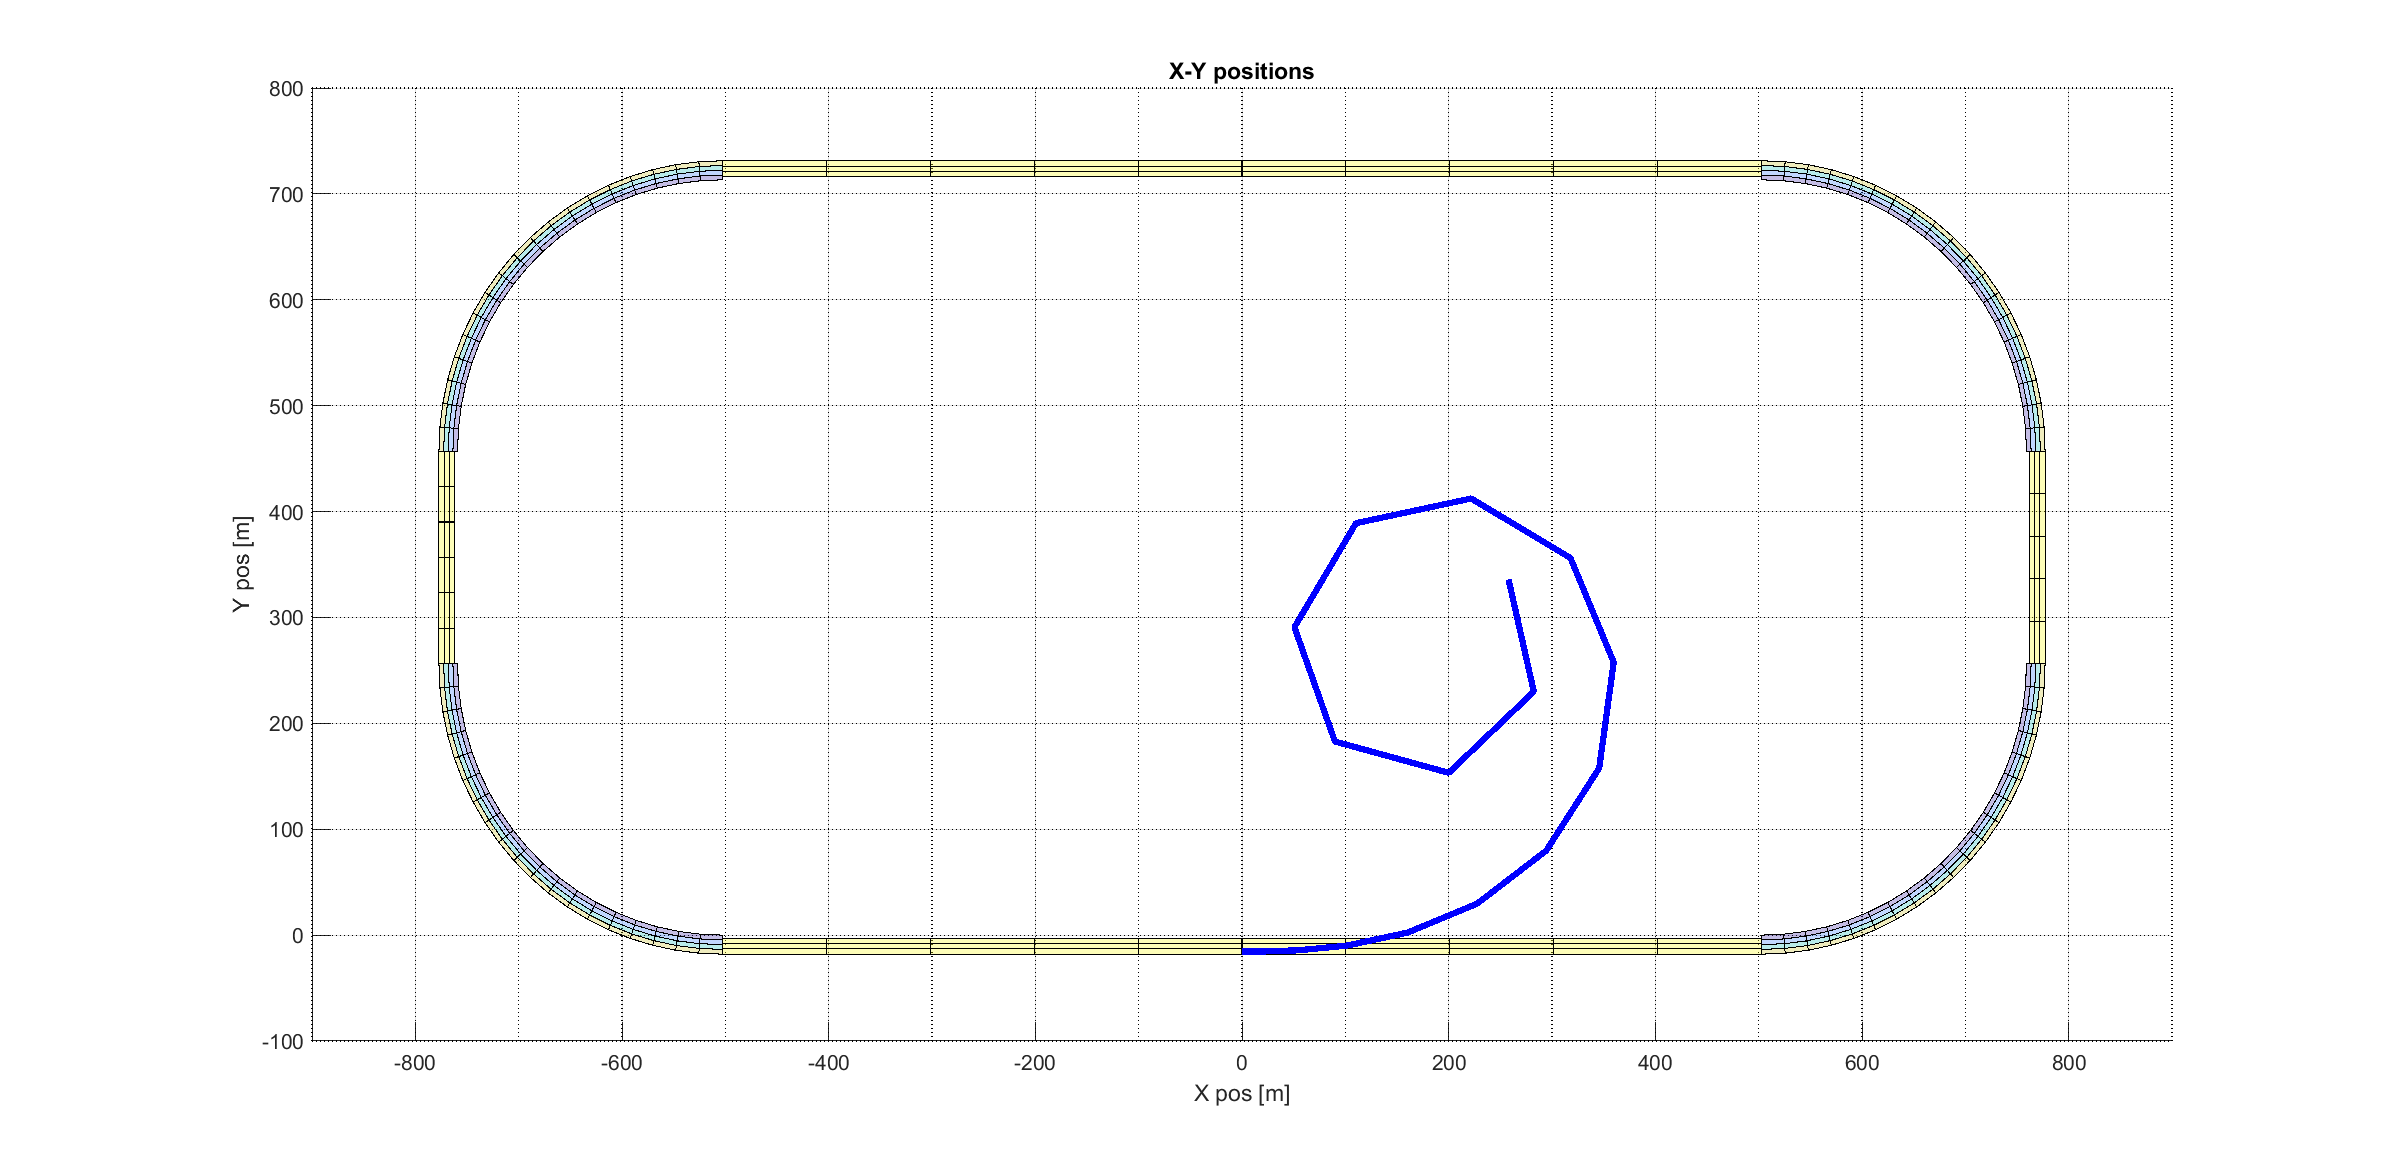
\includegraphics[width=\linewidth]{images/chapter1/simulations/sim5_trajectory.png}
    \caption{Simulation 5 - trajectory of the vehicle}
    \label{fig:sim5_1}
\end{figure}
\begin{figure}[h!]
    \centering
    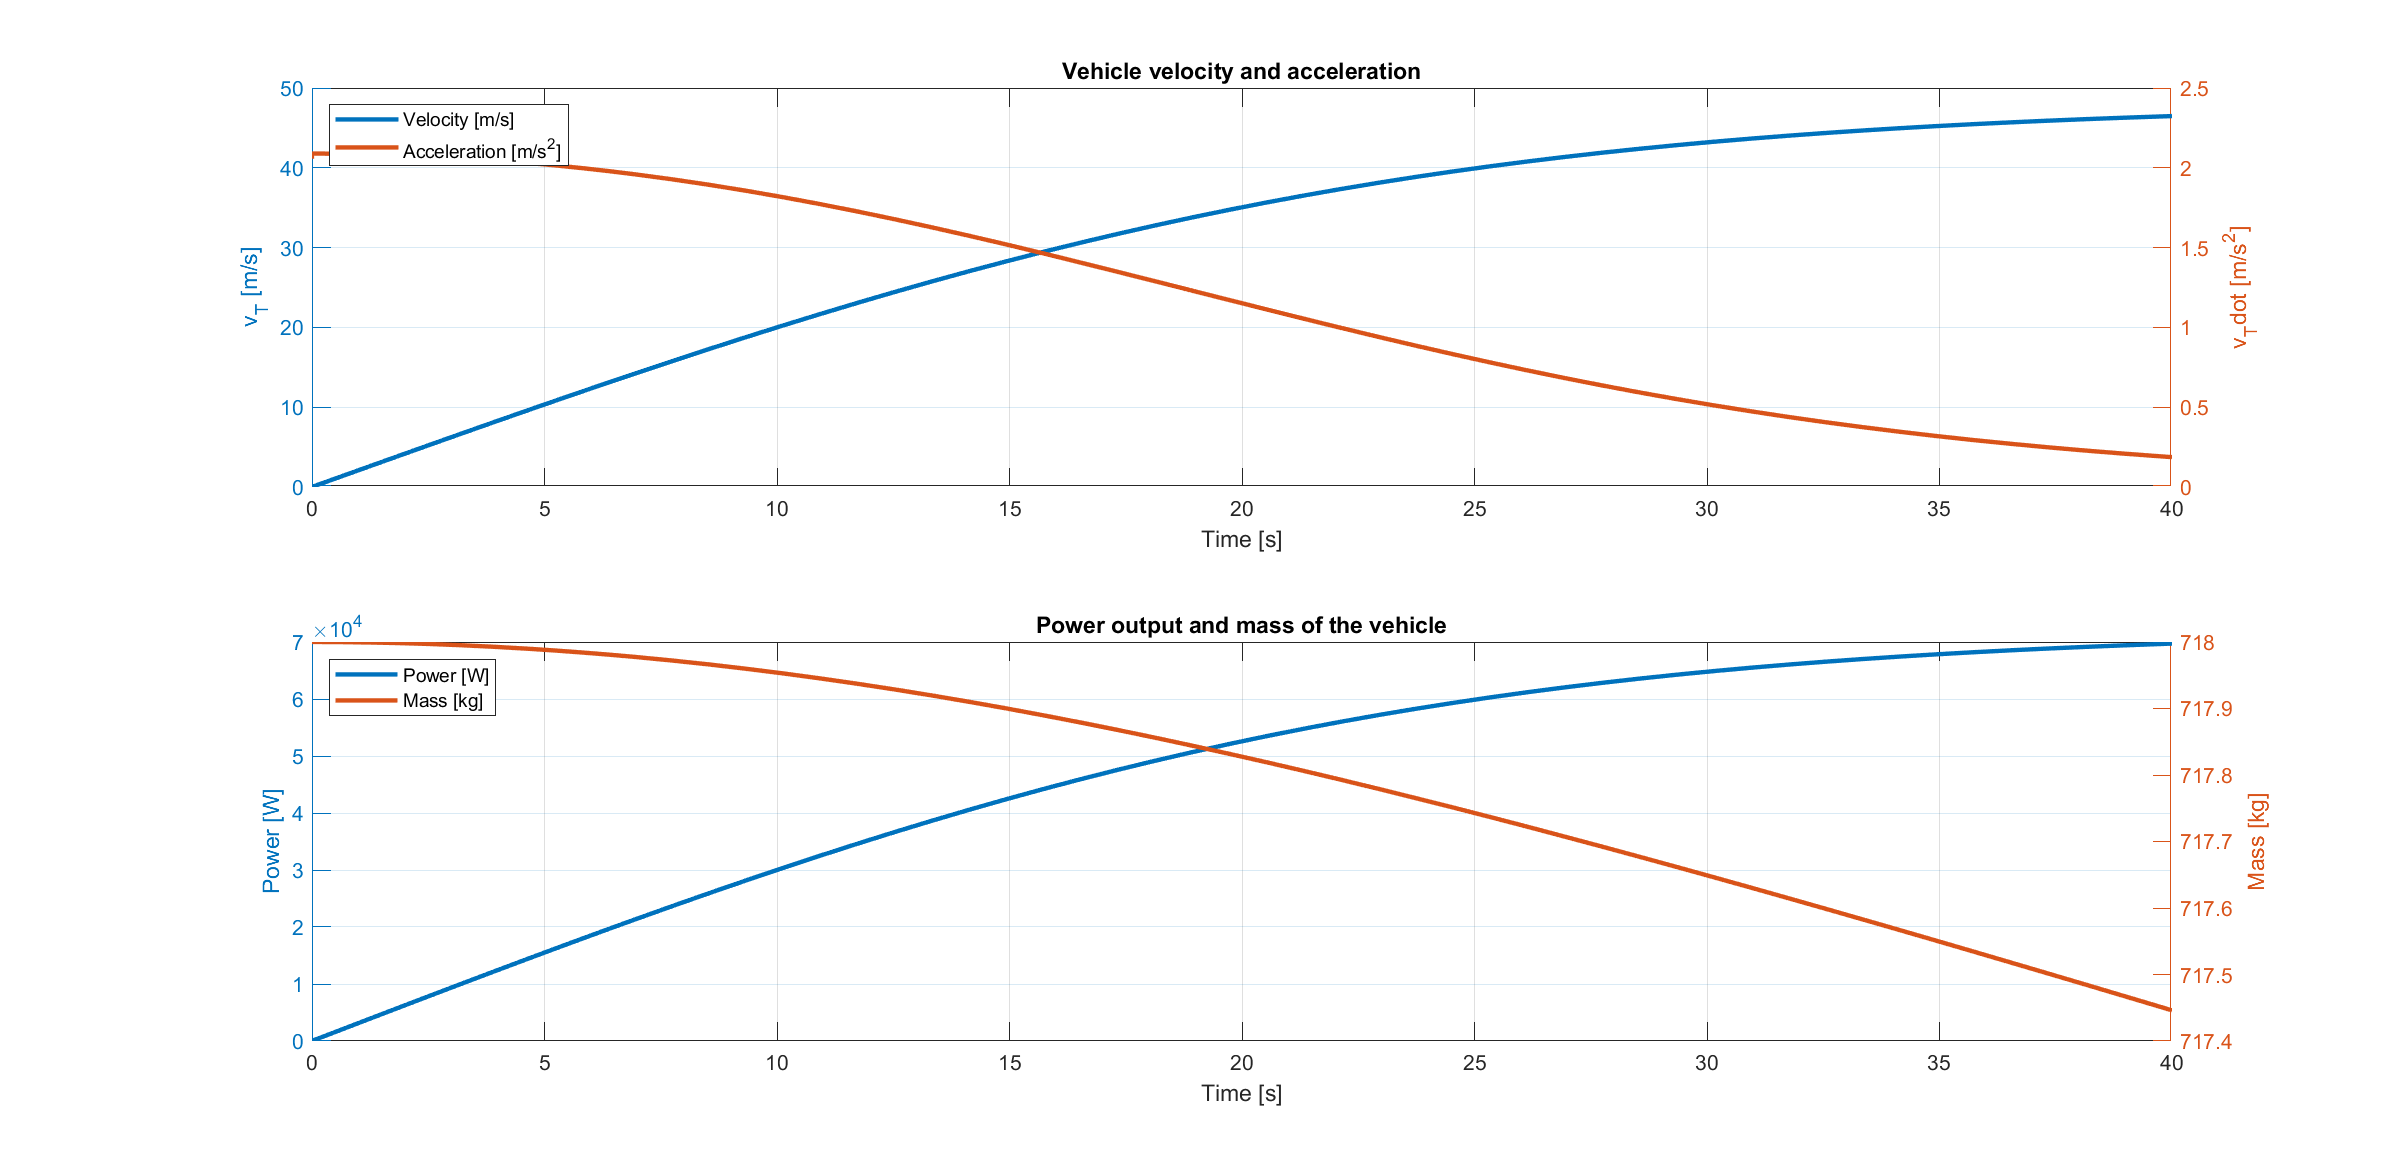
\includegraphics[width=\linewidth]{images/chapter1/simulations/sim5_vel-power.png}
    \caption{Simulation 5 - velocity, acceleration, power and mass figure}
    \label{fig:sim5_2}
\end{figure}
\begin{figure}[h!]
    \centering
    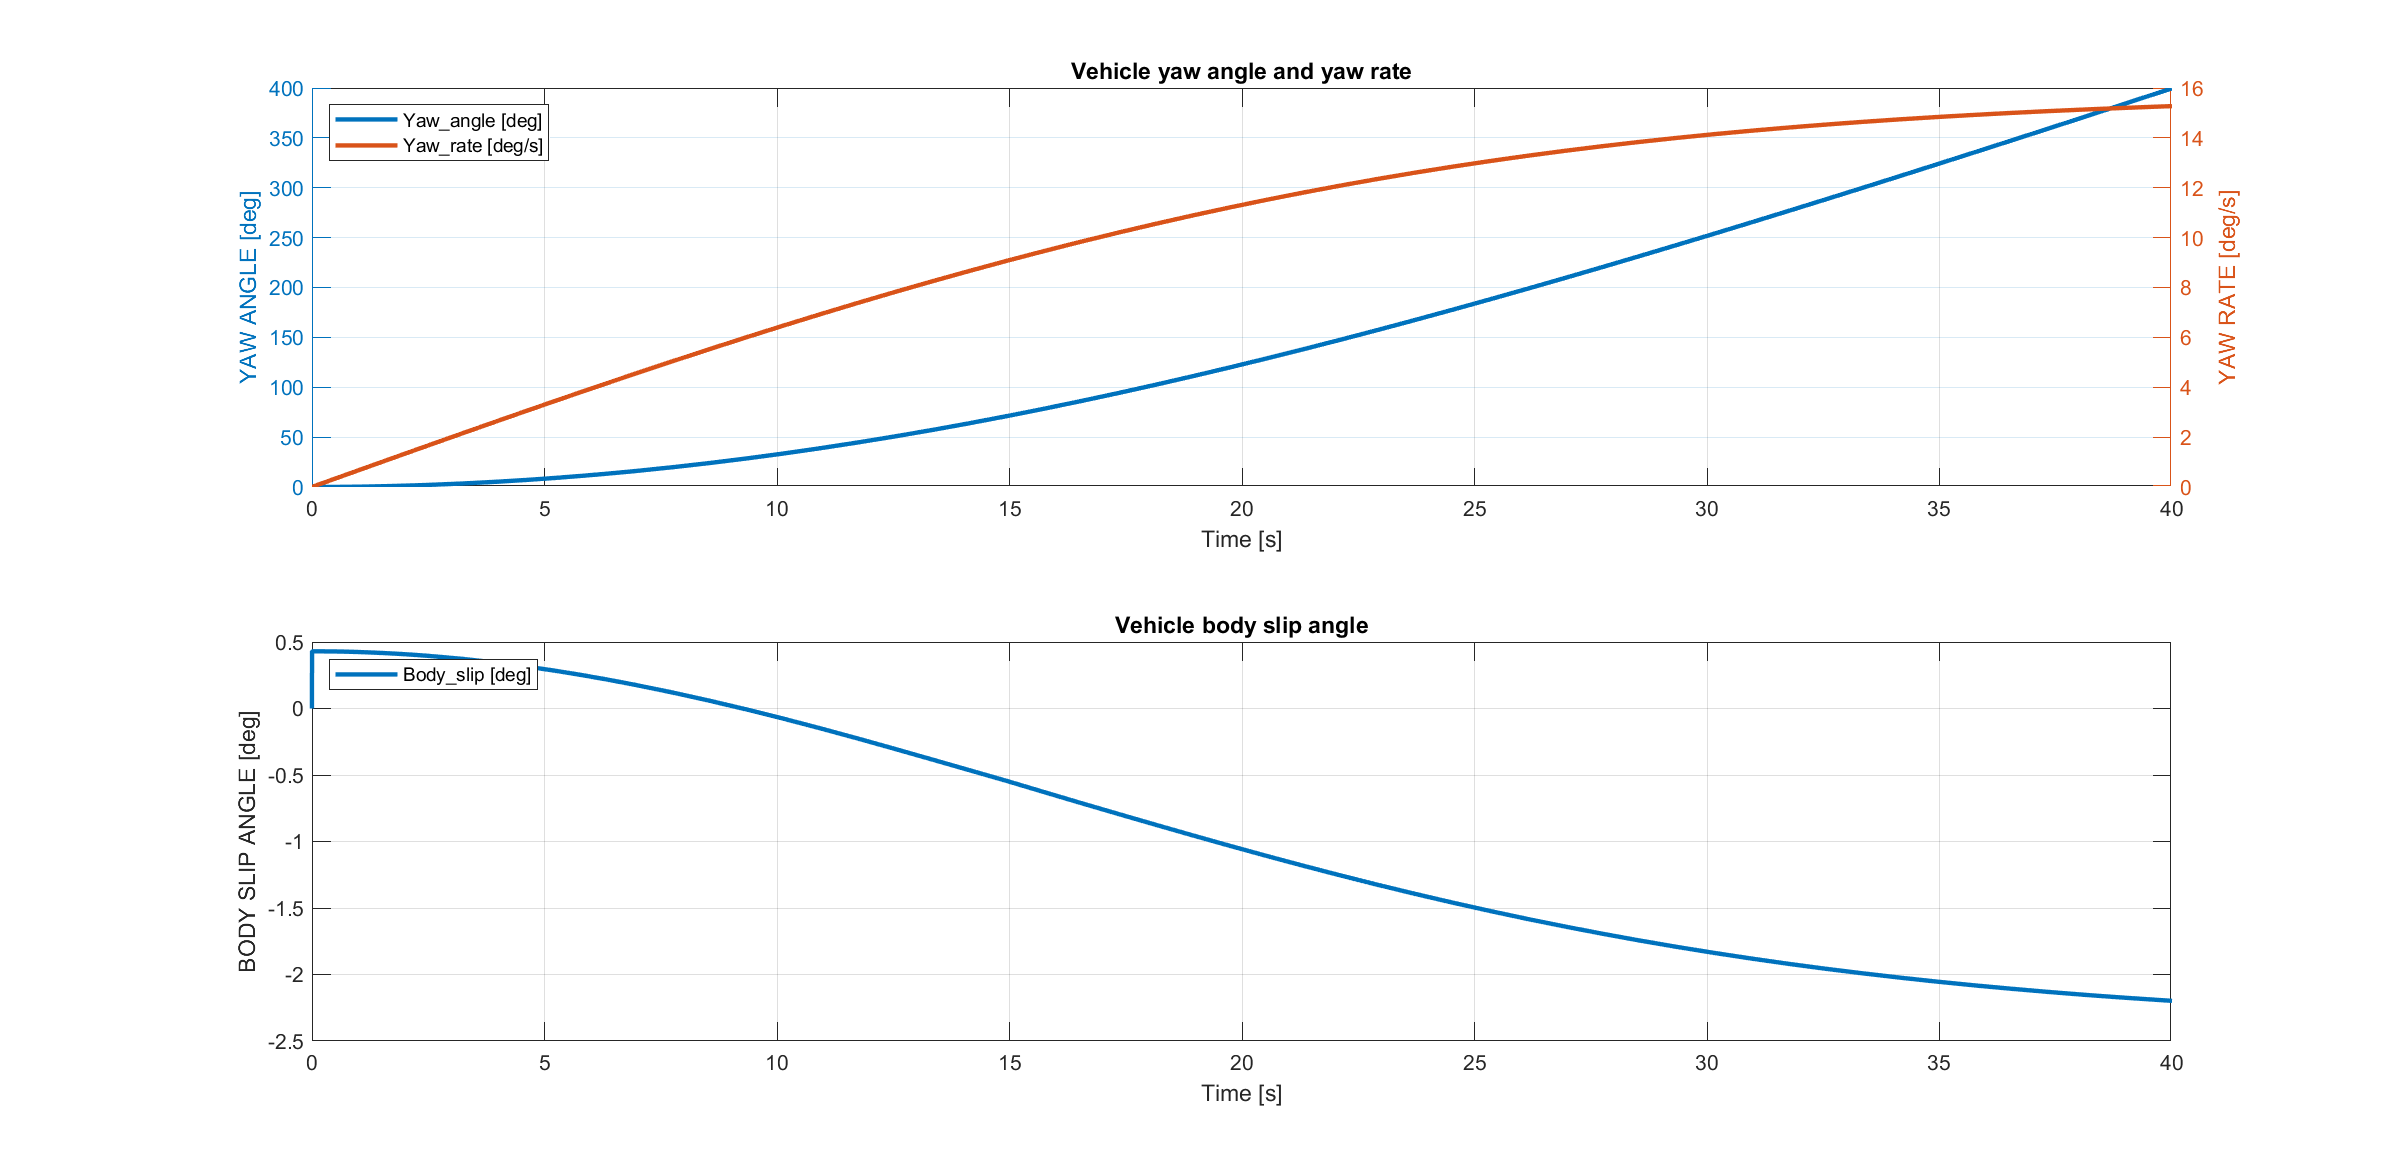
\includegraphics[width=\linewidth]{images/chapter1/simulations/sim5_angles.png}
    \caption{Simulation 5 - angles figure}
    \label{fig:sim5_3}
\end{figure}
\begin{figure}[h!]
    \centering
    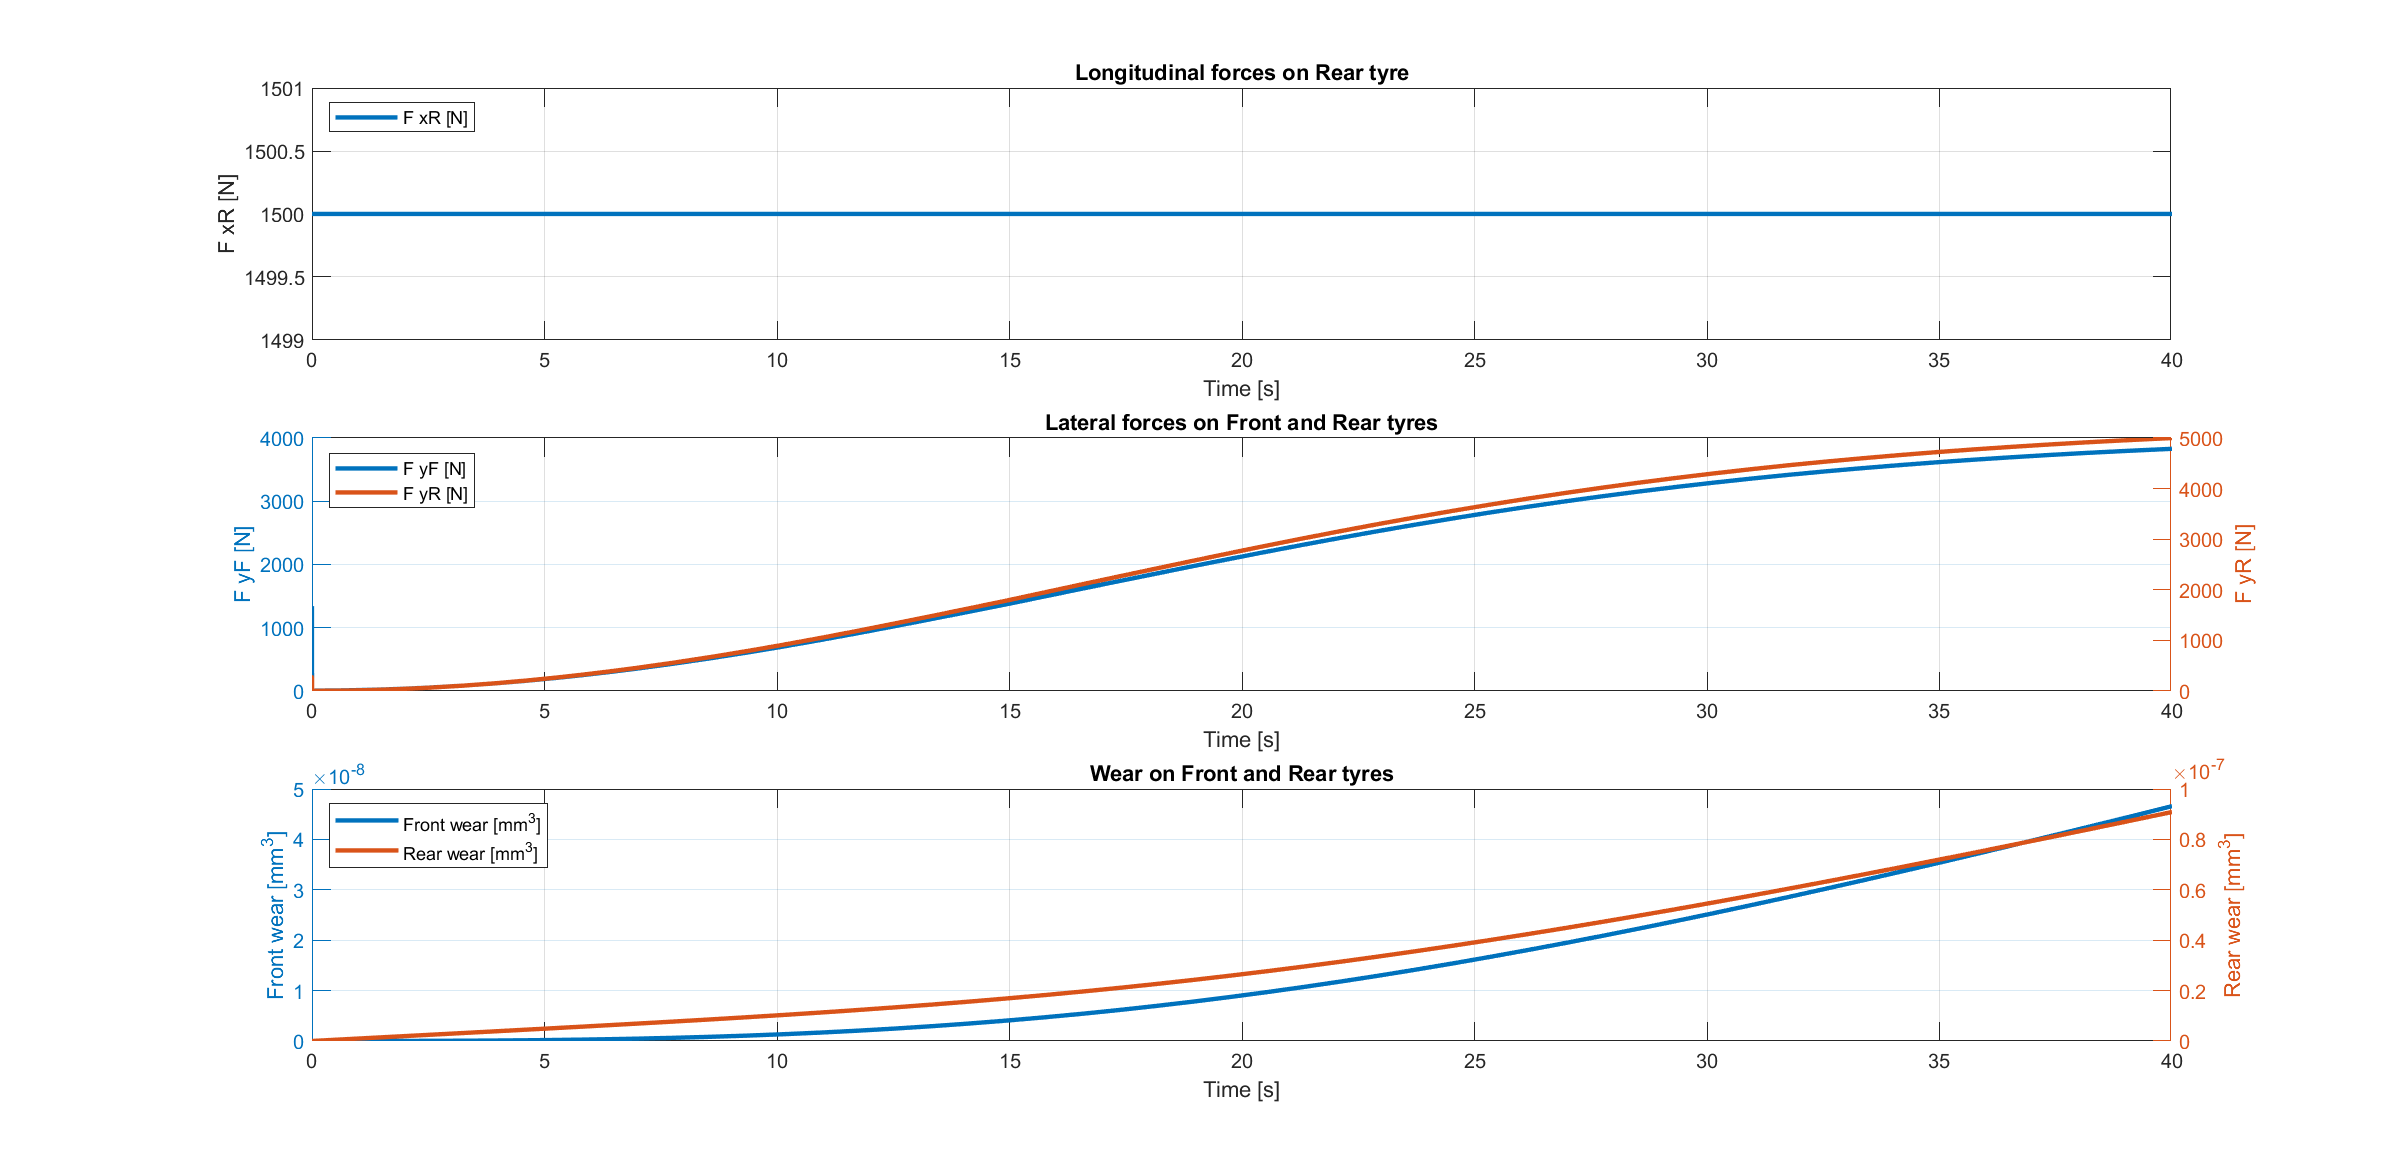
\includegraphics[width=\linewidth]{images/chapter1/simulations/sim5_force-wear.png}
    \caption{Simulation 5 - forces and tyres wear figure}
    \label{fig:sim5_4}
\end{figure}

\subsection{Simulation 6 - Sinusoidal wave path}
The aim of this simulation was to test the correctness of the various figures of merit in a "sinusoidal wave trajectory" situation. The car starts with an initial speed of $0[m/s]$ and then constantly accelerates and steers following a sinusoidal wave with amplitude about $0.02[rad]$ and frequency $0.22[rad/s]$. Provided inputs are $F_x = 500 [N]$, $\delta = 0.02sin(0.22t)$, simulation time = $30 [s]$. \\For the given simulation time and frequency, just a single wave is simulated. The shown figures represent the trajectory, the angles and the lateral forces. Power and mass figures are not shown since consistent with simulation scenario and already shown in previous simulations. All the figures provided exhibit a wave behavior consistent with the simulation data.  
\begin{figure}[h!]
    \centering
    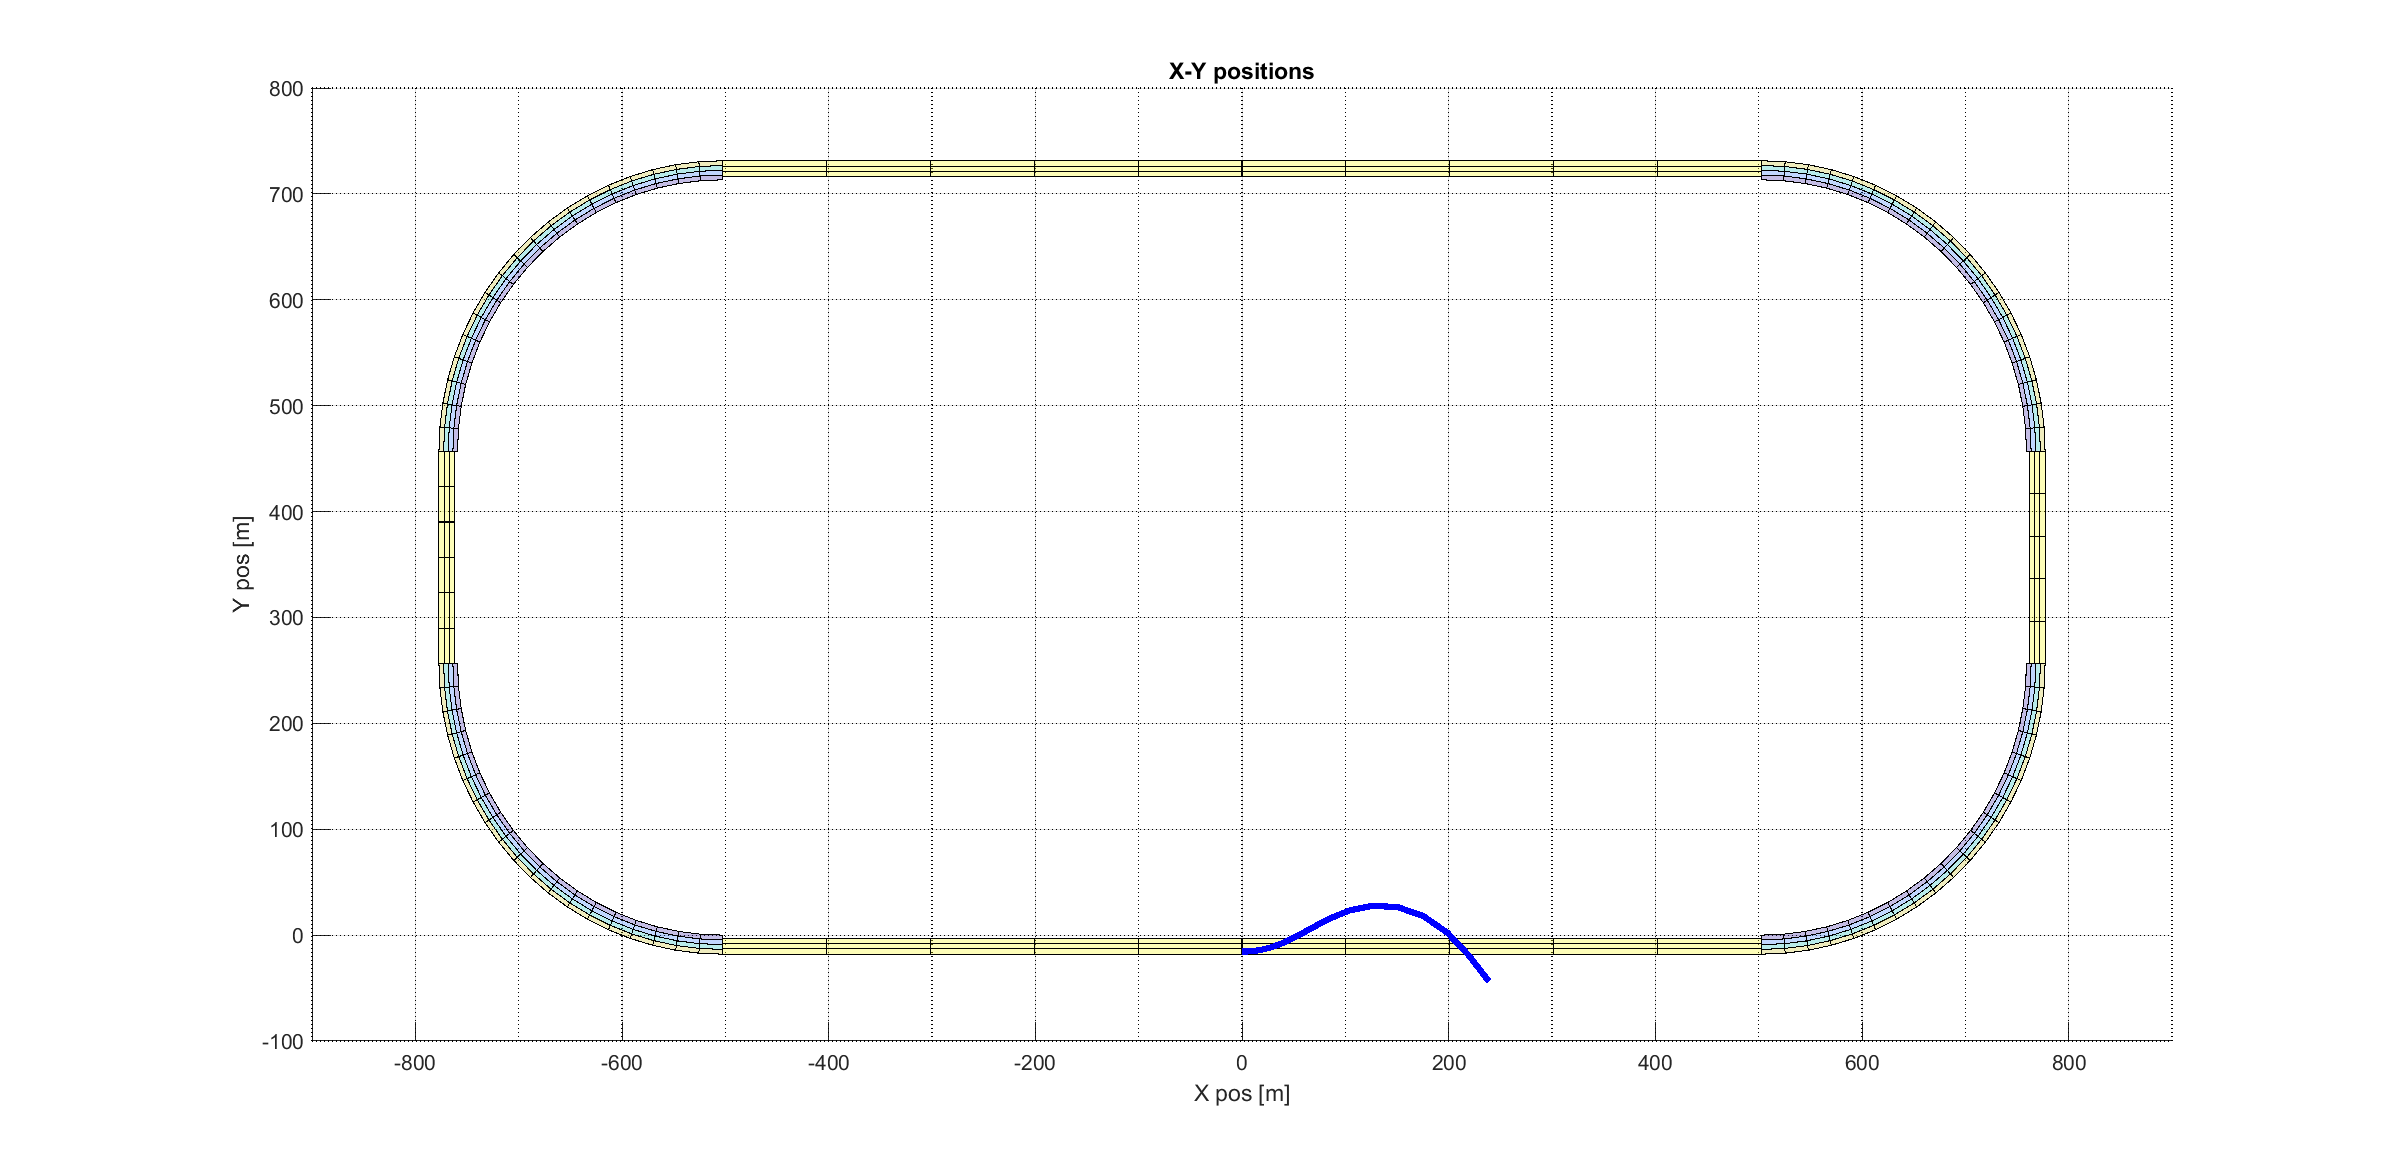
\includegraphics[width=\linewidth]{images/chapter1/simulations/sim6_trajectory.png}
    \caption{Simulation 6 - trajectory of the vehicle}
    \label{fig:sim6_1}
\end{figure}
\begin{figure}[h!]
    \centering
    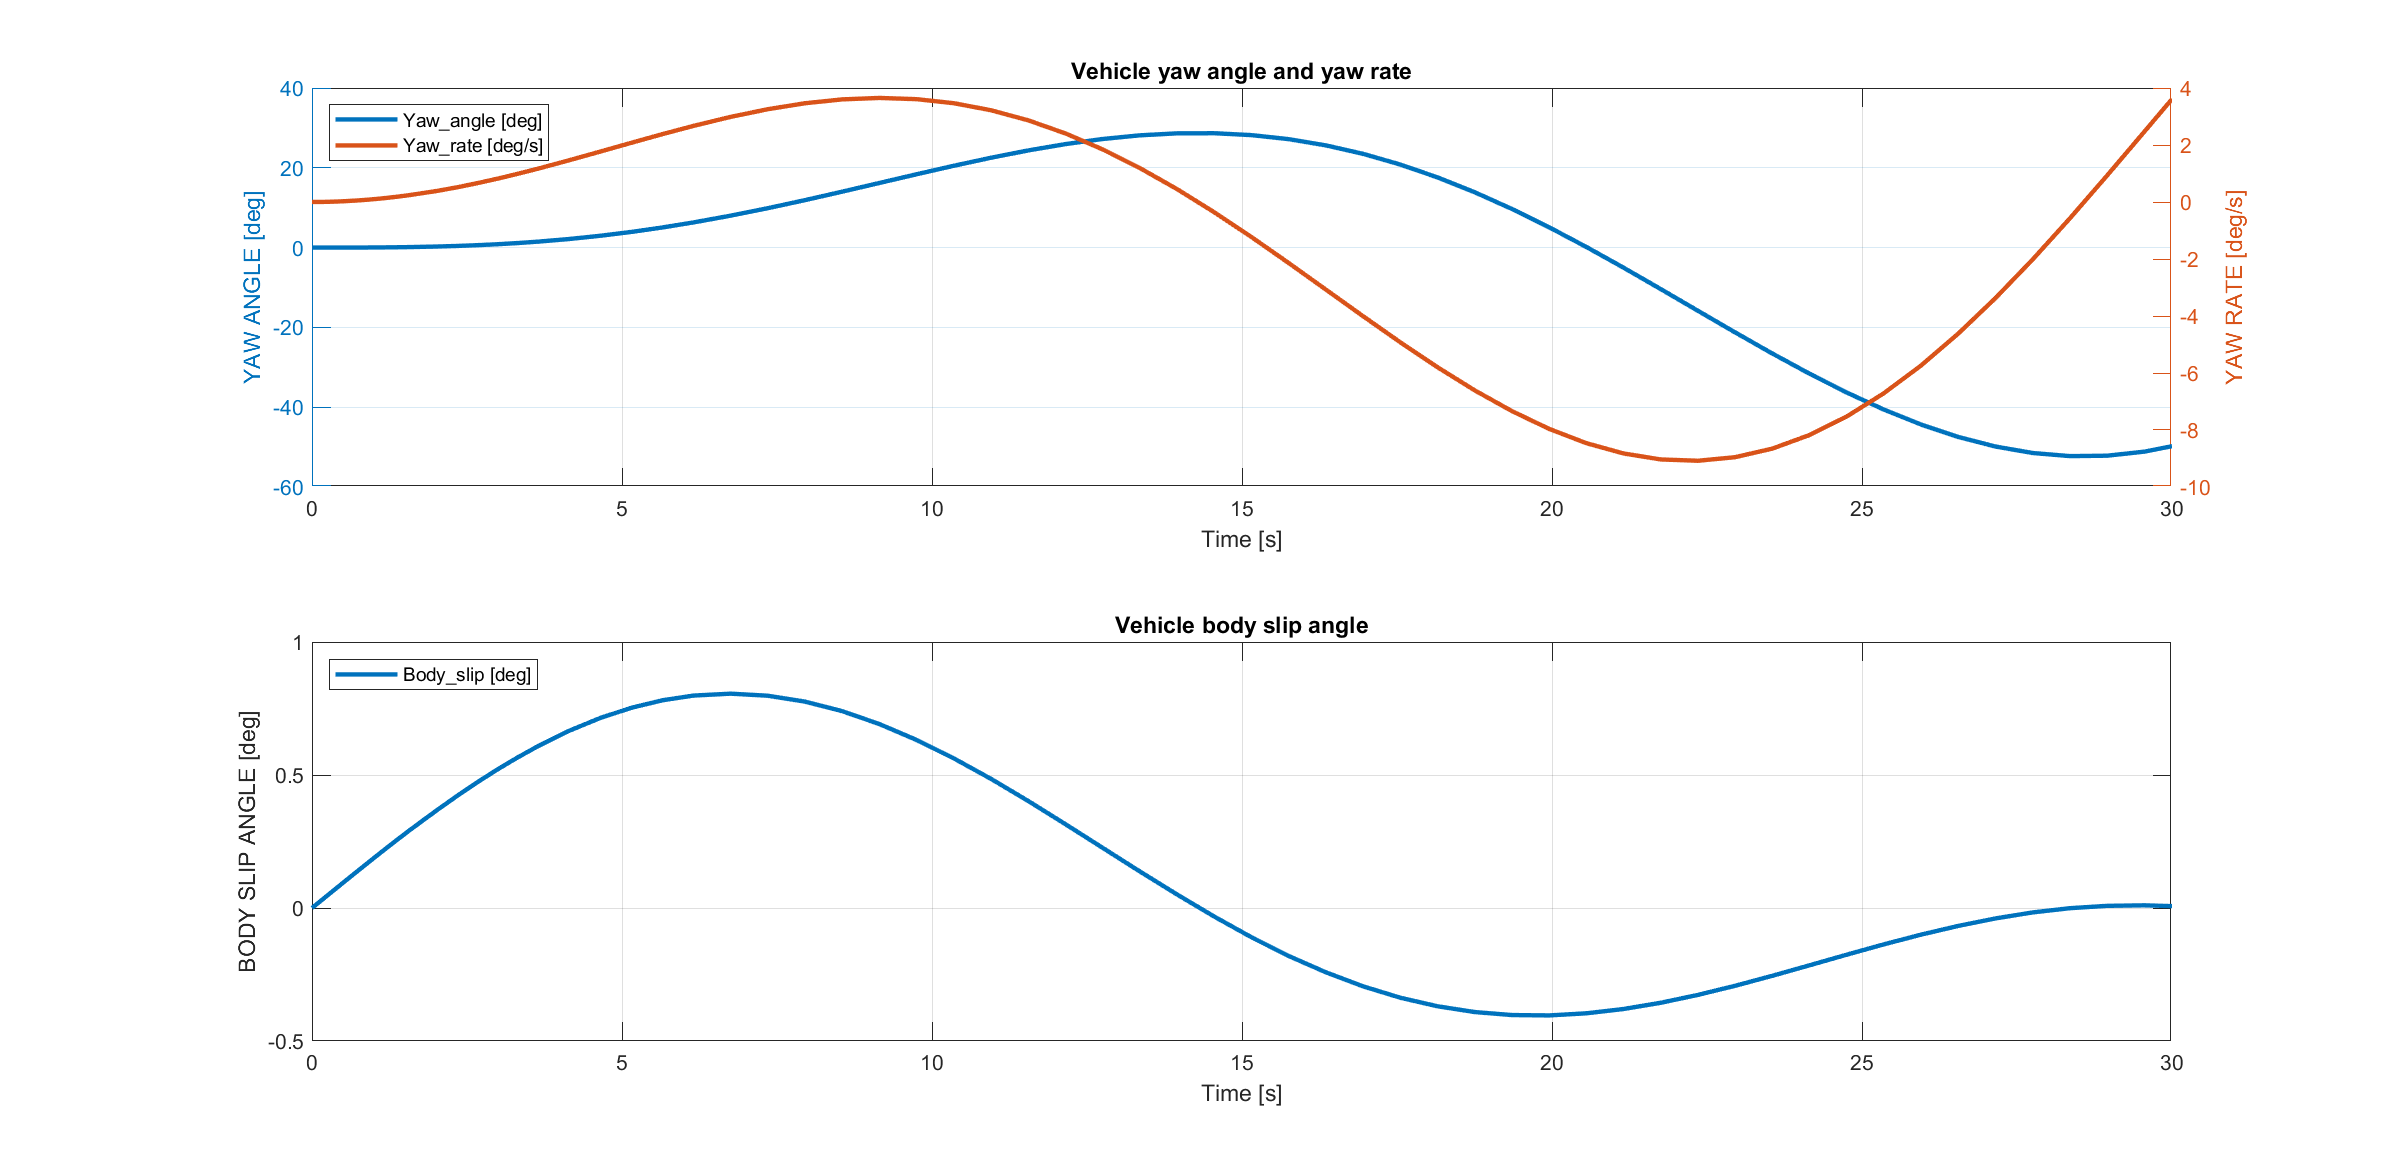
\includegraphics[width=\linewidth]{images/chapter1/simulations/sim6_angles.png}
    \caption{Simulation 6 - angles figure}
    \label{fig:sim6_2}
\end{figure}
\begin{figure}[h!]
    \centering
    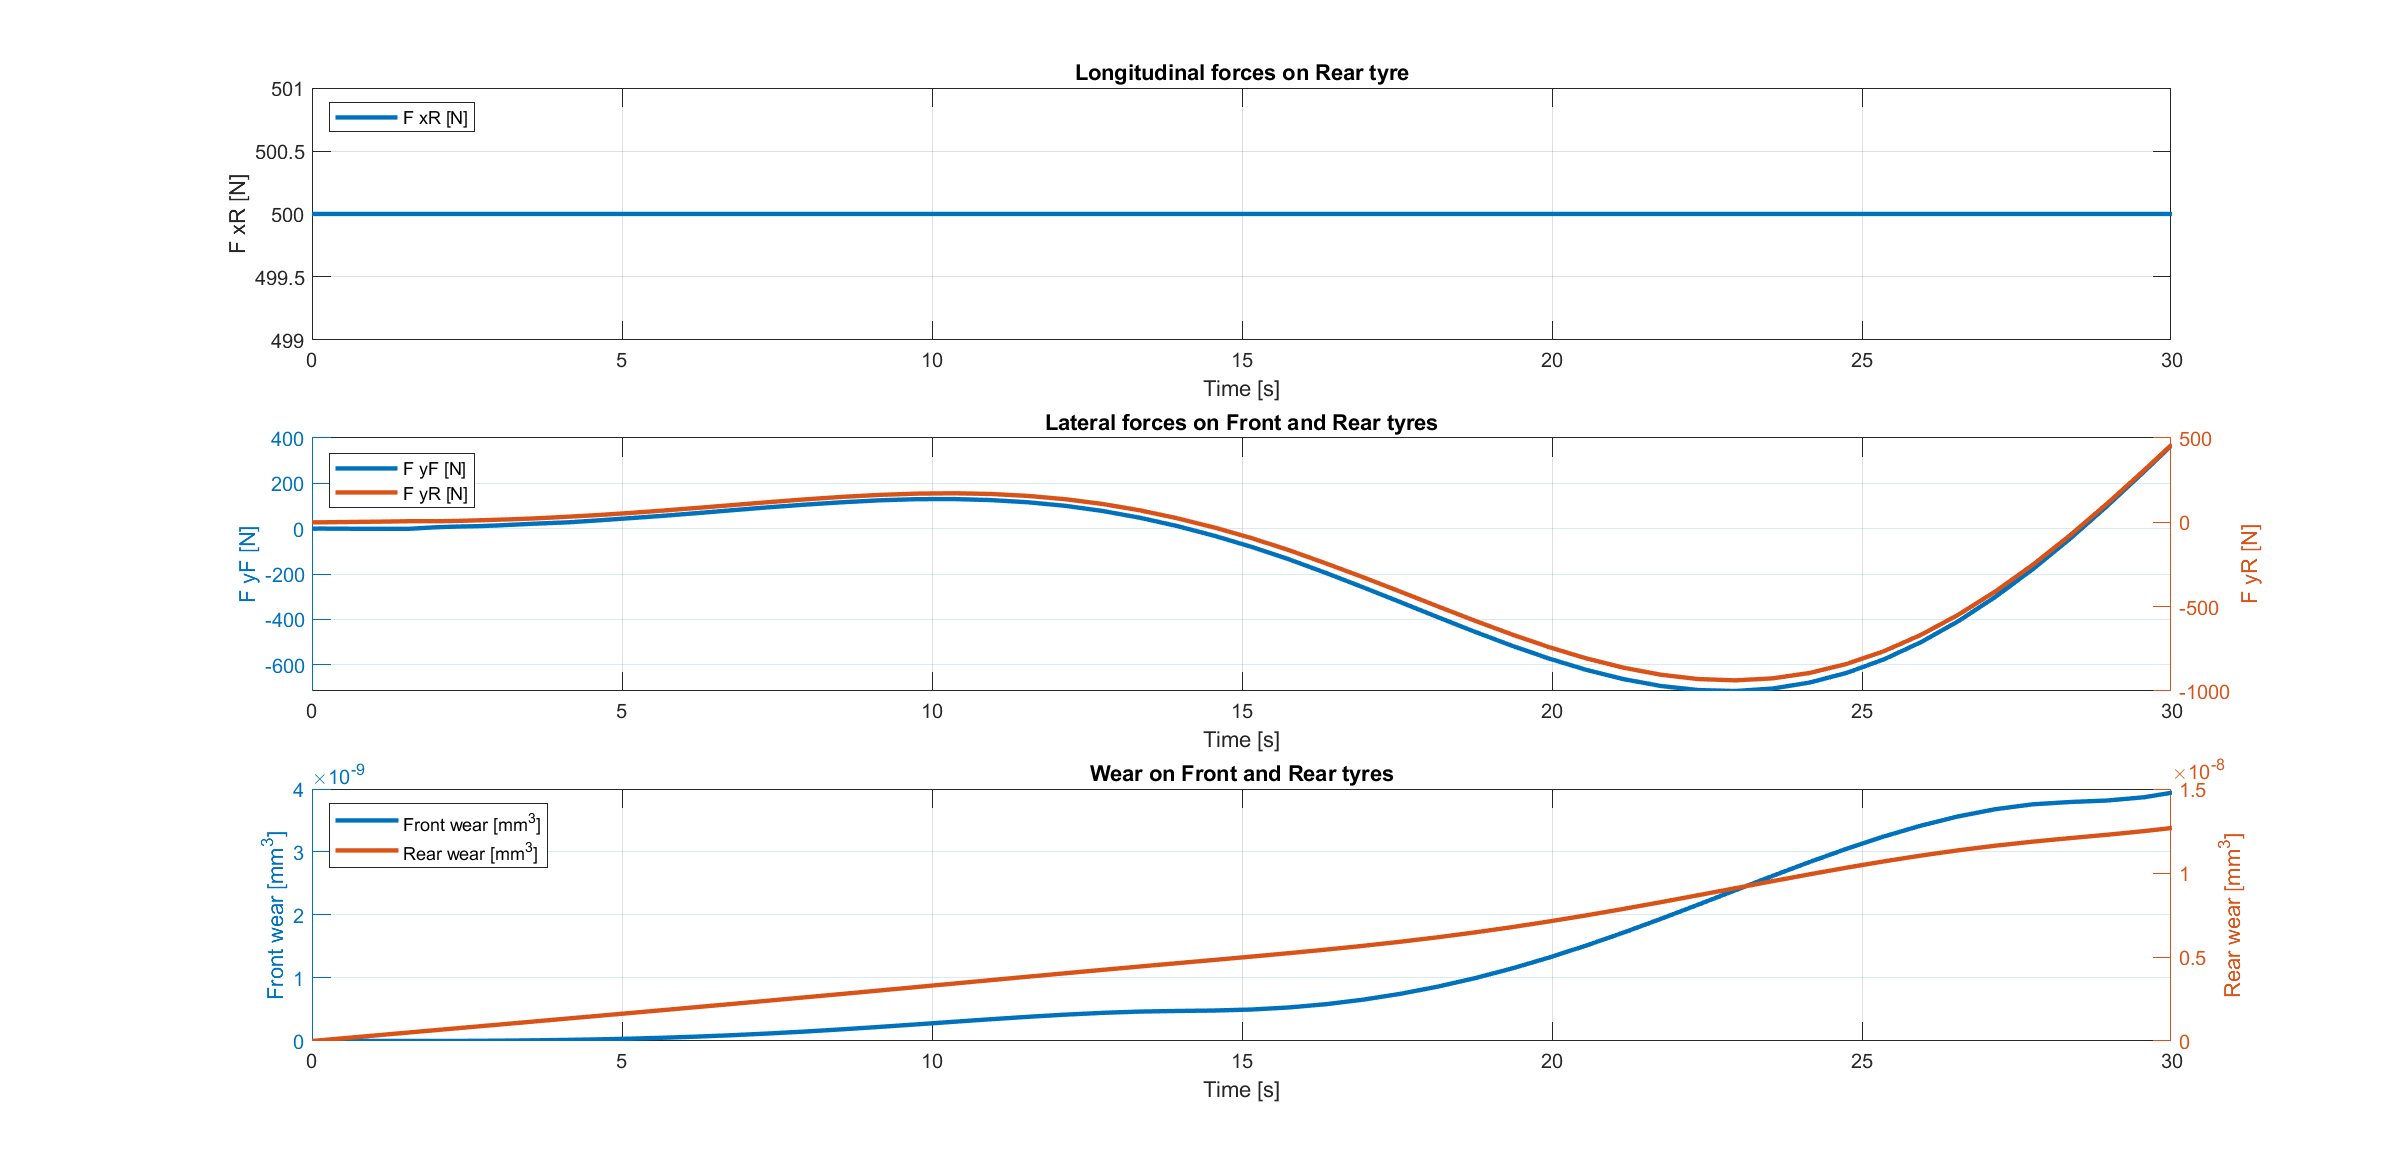
\includegraphics[width=\linewidth]{images/chapter1/simulations/sim6_force-wear.png}
    \caption{Simulation 6 - forces and tyres wear figure}
    \label{fig:sim6_3}
\end{figure}


\subsection{Simulation 7 - Constant speed and increasing steering angle}
The aim of this simulation was to test the correctness of the various figures of merit in a sort of circular trajectory with a constant speed. The car starts with a speed of $30[m/s]$ and after few seconds reaches its desired speed of $50[m/s]$ speed. The applied steering angle is a linear function with slope of $3[deg/s]$ and the simulation is run for $100[s]$: this will result in a final steering angle on the wheels of $30[deg/s]$. The velocity is kept constant by using a simple PID controller. As it is clear also from the figure representing the trajectory, the presented vehicle shows an under-steering behaviour because it enlarges the trajectory even if the applied steering angle is increasing. 
\begin{figure}[h!]
    \centering
    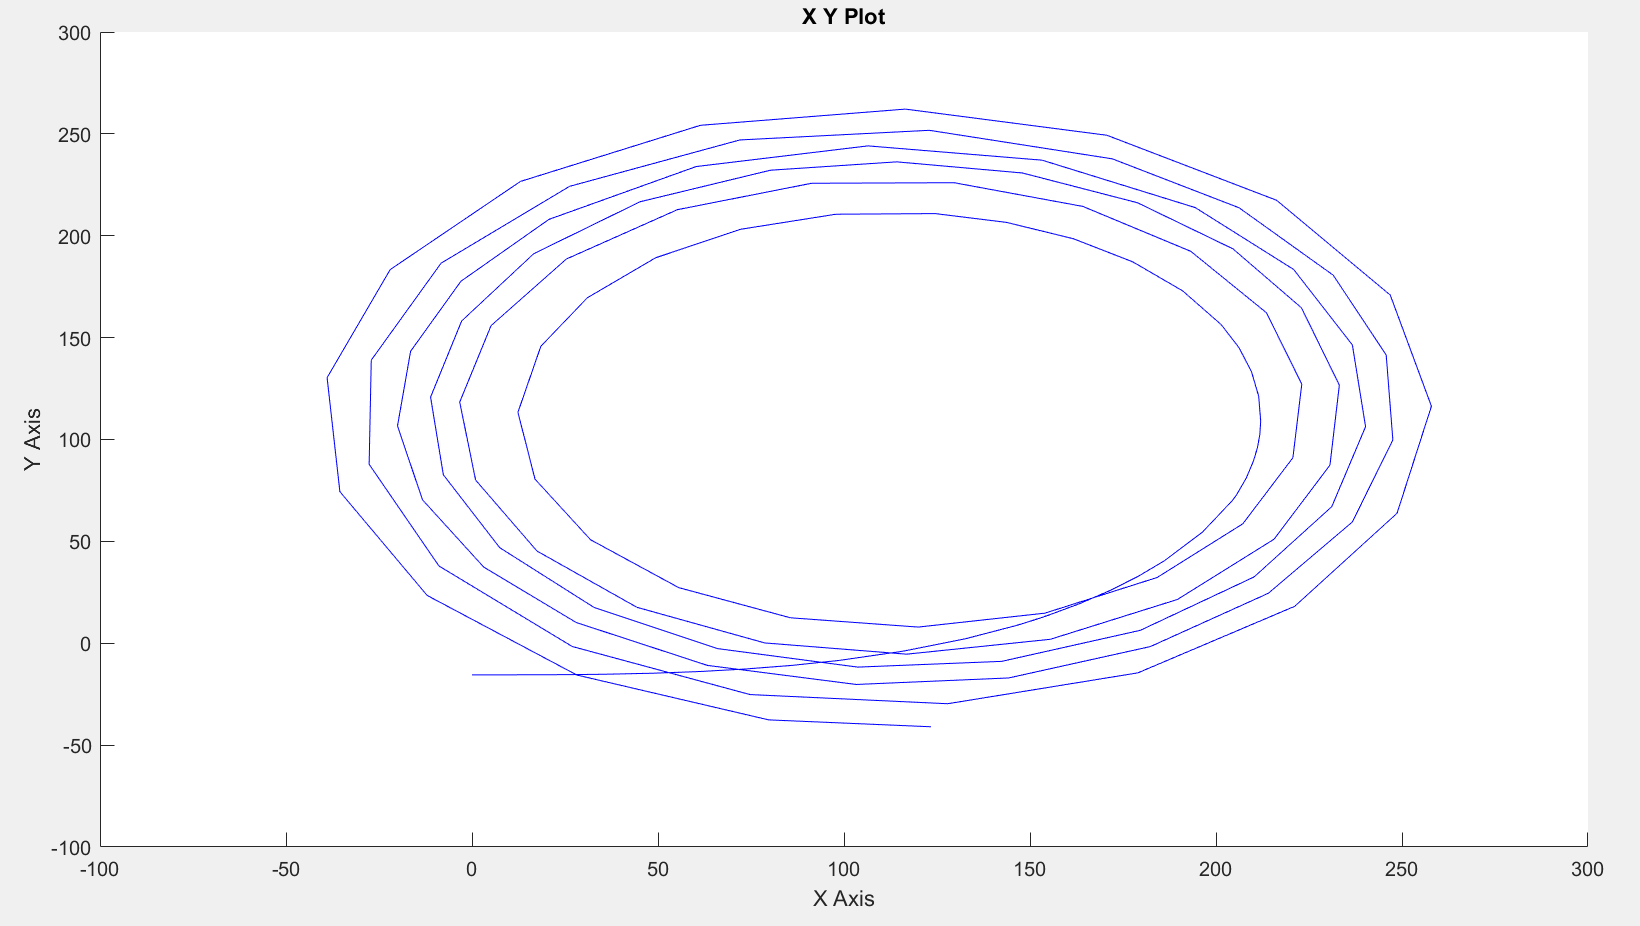
\includegraphics[width=\linewidth]{images/chapter1/simulations/sim7_trajectory2.png}
    \caption{Simulation 7 - trajectory of the vehicle}
    \label{fig:sim7_1}
\end{figure}
\begin{figure}[h!]
    \centering
    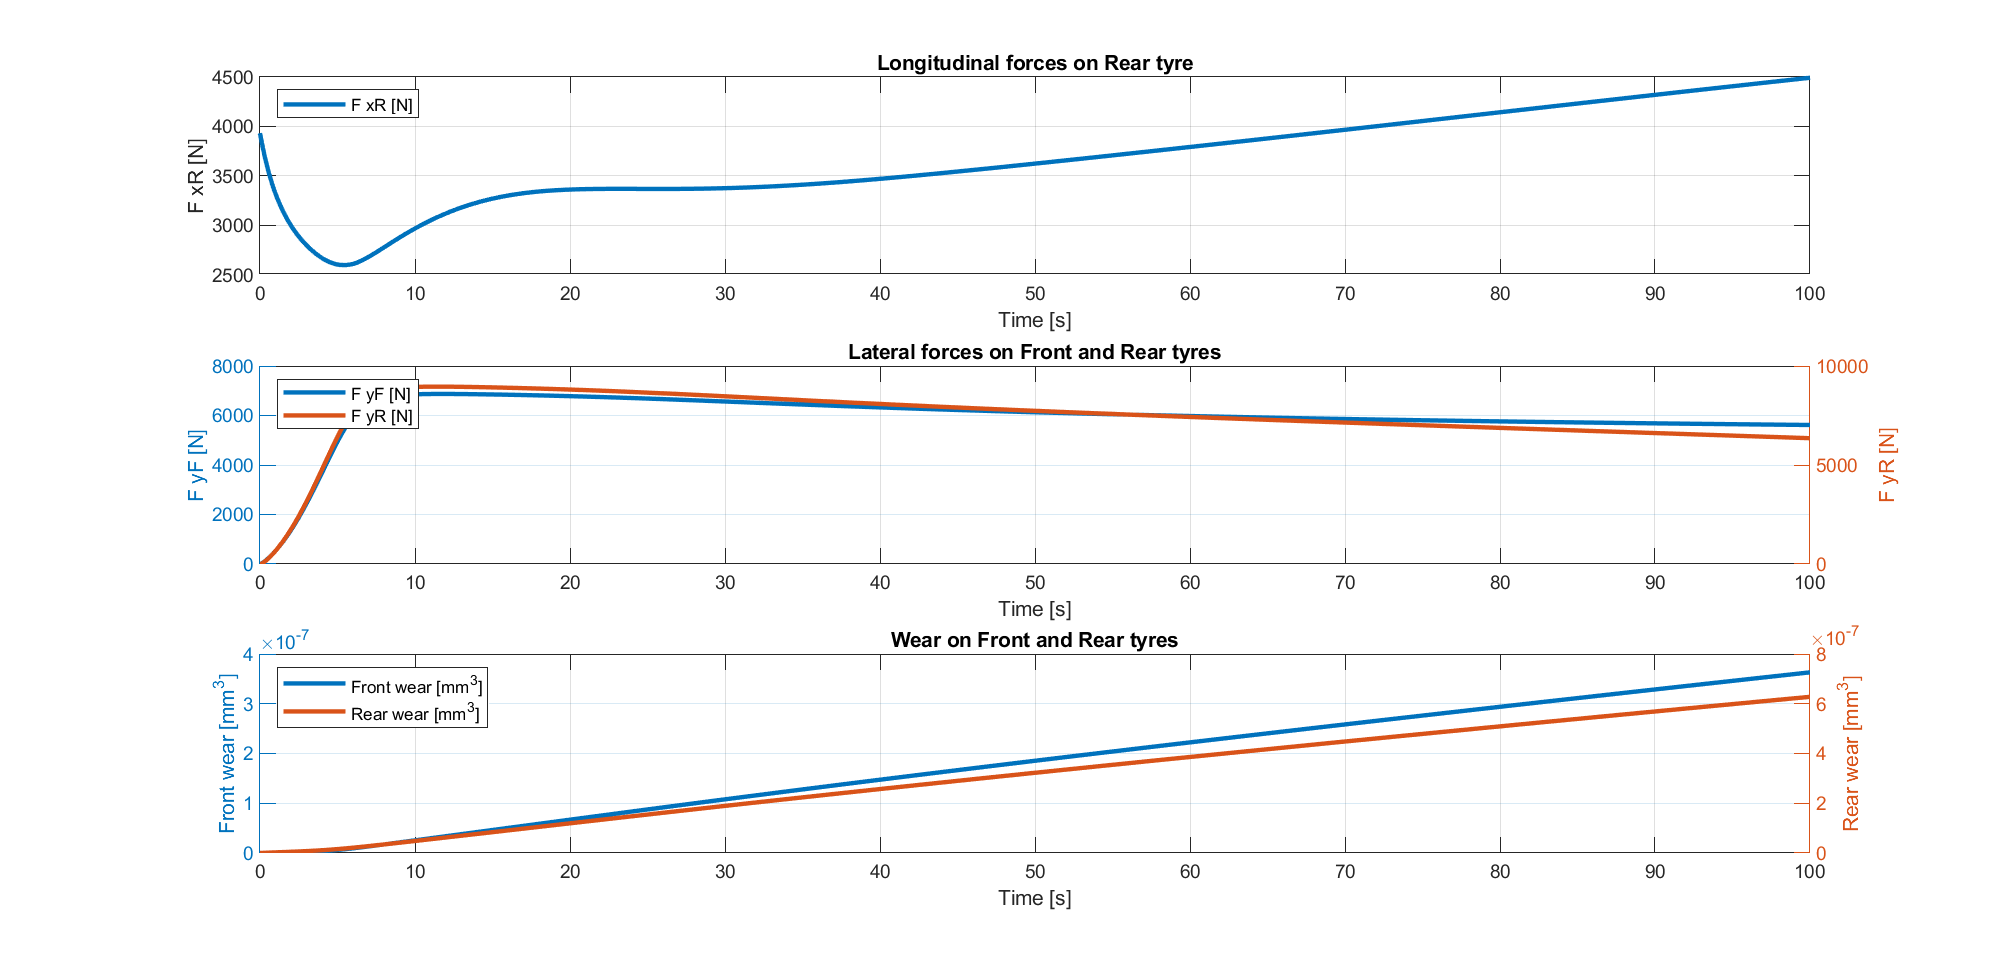
\includegraphics[width=\linewidth]{images/chapter1/simulations/sim7_force-wear.png}
    \caption{Simulation 7 - forces and tyres wear figure}
    \label{fig:sim7_2}
\end{figure}
\begin{figure}[h!]
    \centering
    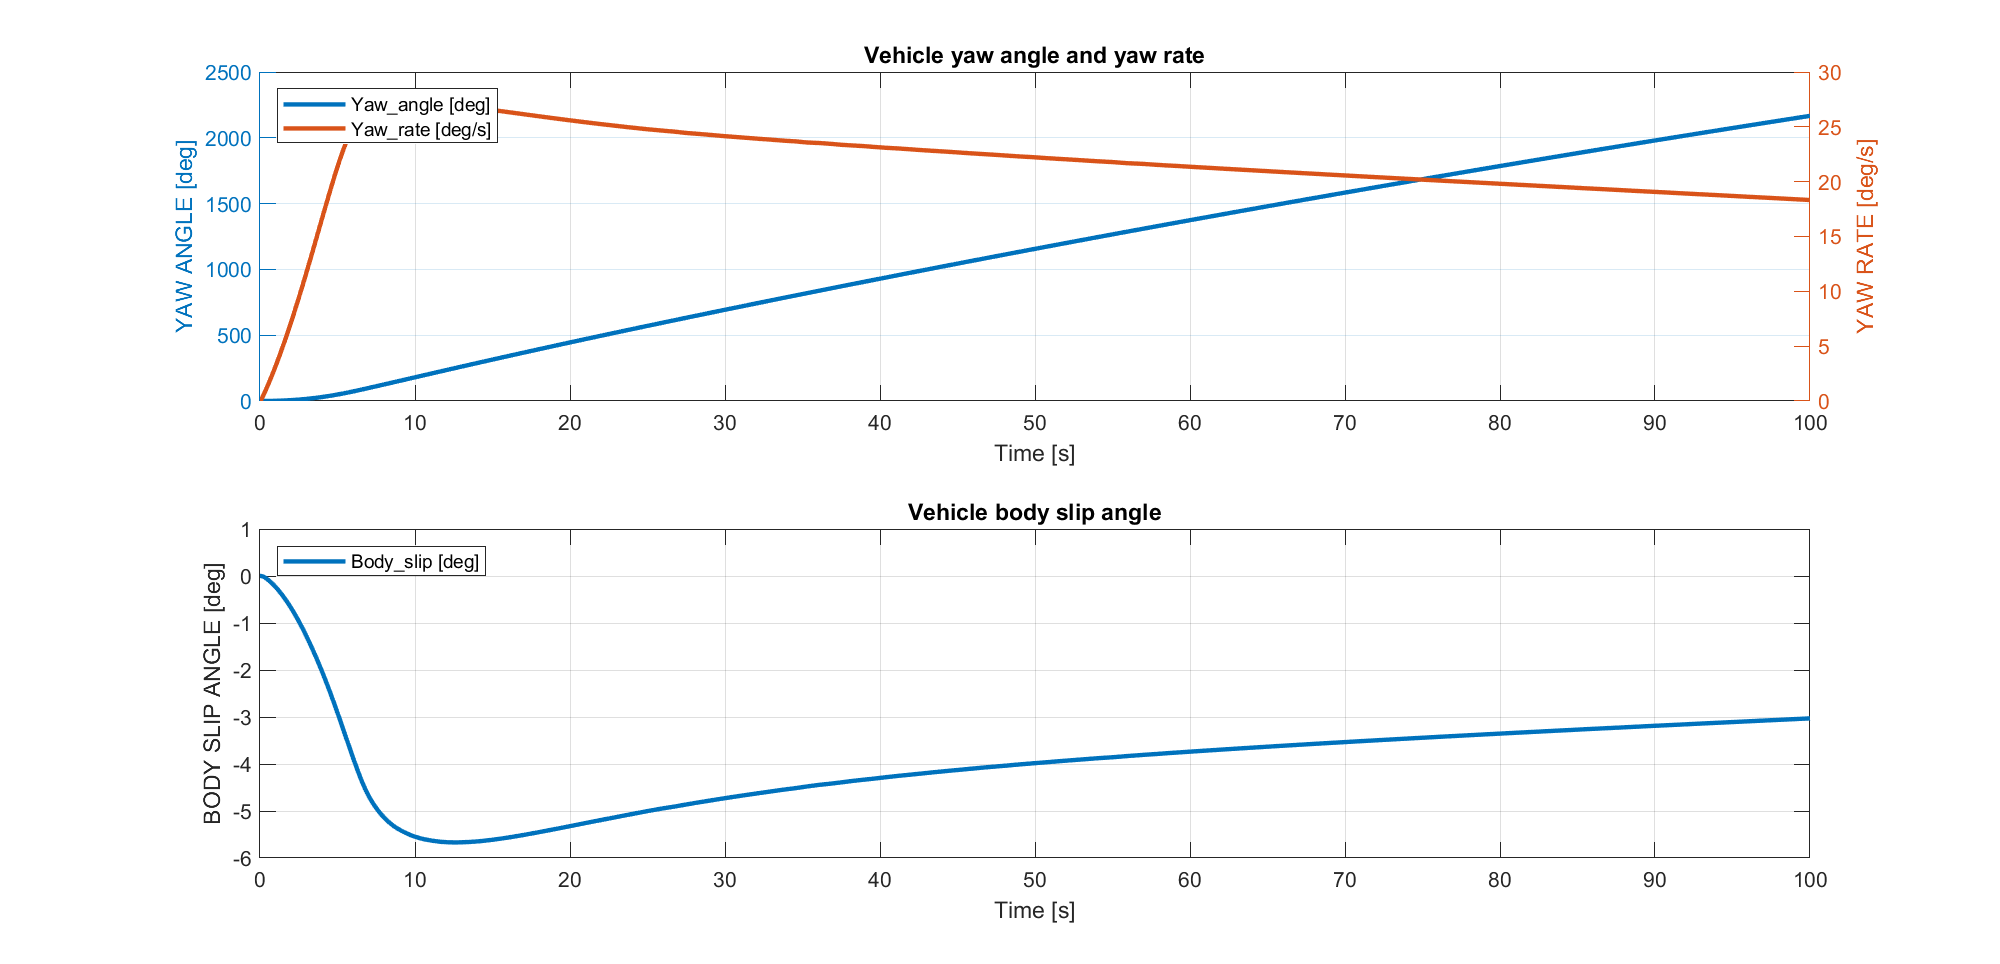
\includegraphics[width=\linewidth]{images/chapter1/simulations/sim7_angles.png}
    \caption{Simulation 7 - angles figure}
    \label{fig:sim7_3}
\end{figure}
\begin{figure}[h!]
    \centering
    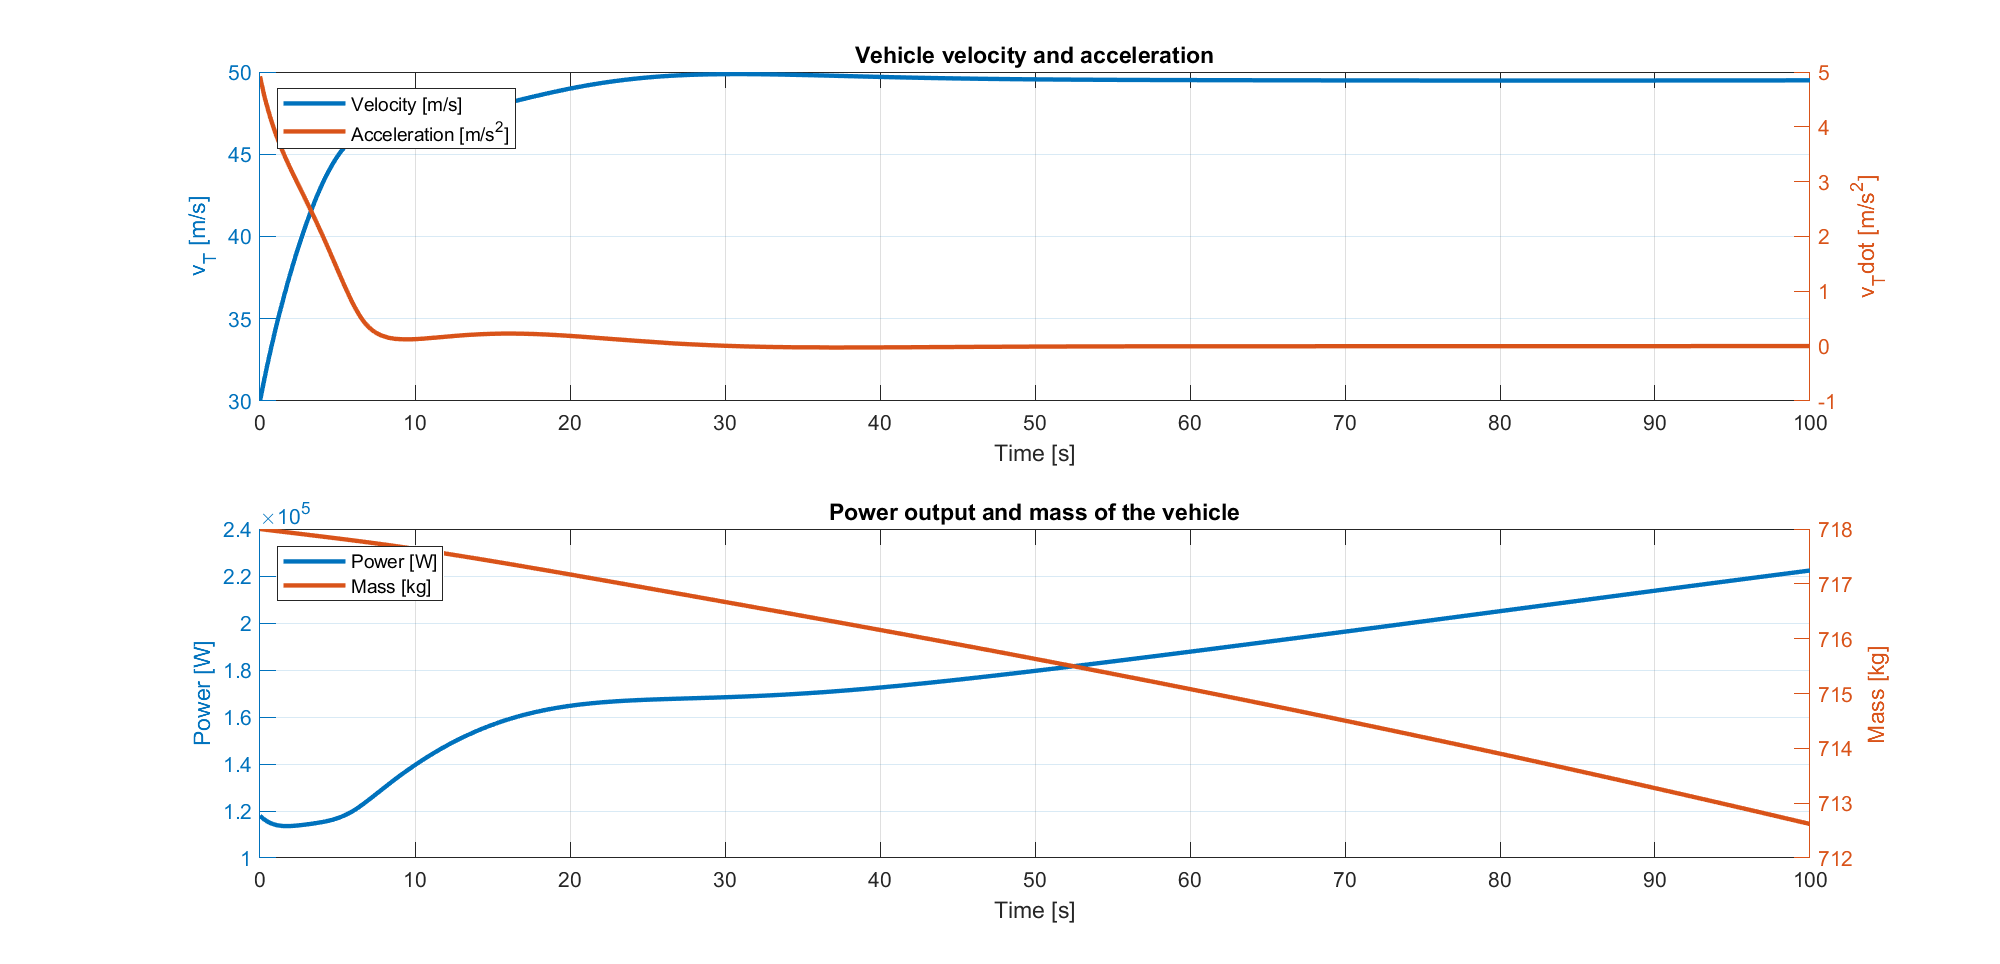
\includegraphics[width=\linewidth]{images/chapter1/simulations/sim7_vel-power.png}
    \caption{Simulation 7 - velocity, acceleration, power and mass figure}
    \label{fig:sim7_4}
\end{figure}

\clearpage
\newpage

\chapter{Control}
In this chapter controllers are realized in order to achieve the possibility for the vehicle to follow a given trajectory according to a certain velocity profile. For this goal, two different controllers have been realized: a longitudinal controller and a lateral one. 
\\Both of them were designed on a linearized version of our model with linear tyre model and then tested on the real simulator.

\section{Linearized model}
Here the linearized model with linear tyre model is presented.
\\First of all in the linear tyre model the lateral forces of the tyres are proportional to the slip angles up to a coefficient called cornering stiffness coefficient ($C_i$). This was estimated by looking at the mean vertical forces on the tyres and looking the slip-lateral force relation in the graph of the Pacejka model. As can be seen from figures \ref{fig:Cf} and \ref{fig:Cr}, by using a $C_F = 100000$ [N/rad] and $C_R = 120000$ [N/rad], linear tyre model well approximate non-lateral one specifically for small slips angles: the small angle assumption is exploited for the linearization process. The figures are drawn with respect to the mean value of vertical load on the tyres, respectively 4000 [N] for the front one and 5200 [N] on the rear.
\\Given the model presented so far without considering banking and aerodynamic force:
\begin{equation}
\begin{aligned}
x1 = x\\
x2 = y\\
x3 = \psi\\
x4 = v_T\\
x5 = \beta\\
x6 = \dot{\psi}\\\\
\dot{x_1} = x_4 cos(x_3 + x_5)\\
\dot{x_2} = x_5 sin(x_3 + x_5)\\
\dot{x_3} = x_6 \\
\dot{x_4} = \frac{F_{xF} cos(x_5-\delta) + F_{xR} cos(x_5) + F_{yF} sin(x_5-\delta) + F_{yR} sin(x_5)}{m_T} \\
\dot{x_5} = \frac{-F_{xF} sin(x_5-\delta) - F_{xR} sin(x_5) + F_{yF} cos(x_5-\delta) + F_{yR} cos(x_5) - m_T x_4 x_6}{m_T x_4} \\
\dot{x_6} = \frac{F_{xF} a sin(\delta) + F_{yF} a cos(\delta) - F_{yR} b}{I_T} \\\\\\
\alpha_F = arctan(\frac{x_4 sin(x_5) + ax_6}{x_4 cos(x_5)}) - \delta\\
\alpha_R = arctan(\frac{x_4 sin(x_5) - bx_6}{x_4 cos(x_5)}) \\\\
\end{aligned}
\end{equation}
We can linearize it by choosing a specific operating point where we can assume that the vehicle is travelling along a straight path following a constant longitudinal velocity:
\begin{equation}
\begin{aligned}
\text{Operating point for states}\\
x1 = x_{op}\\
x2 = y_{op}\\
x3 = \psi_{op} = 0\\
x4 = v_{T\_op} = v_{T, const}\\
x5 = \beta_{op} = 0\\
x6 = \dot{\psi}_{op} = 0\\\\
\text{Operating point for inputs - considering also linear lateral forces}\\
\delta_{op} = 0\\
F_{xF\_op} = 0\\
F_{xR\_op} = 0\\
F_{yF\_op} = 0\\
F_{yR\_op} = 0\\
\end{aligned}
\end{equation}
Expanding the system in a Taylor series:
\begin{equation}
\begin{aligned}
f_{lin} = f(x_{op},u_{op}) + \nabla f(x_{op},u_{op}) [x - x_{op}  |  u - u_{op}]'
\end{aligned}
\end{equation}
And considering linear tyre model and linear version of the slip angles:
\begin{equation}
\begin{aligned}
F_{yF} = -C_F \alpha_F\\
F_{yR} = -C_R \alpha_R\\
\alpha_F = x_5 + \frac{a}{v_{T, const}}x_6 - \delta\\
\alpha_R = x_5 - \frac{b}{v_{T, const}}x_6 \\\\
\end{aligned}
\end{equation}
We obtain the linearized model:
\begin{equation}
\begin{aligned}
x1 = x\\
x2 = y\\
x3 = \psi\\
x4 = v_T\\
x5 = \beta\\
x6 = \dot{\psi}\\\\
\dot{x_1} = x_4\\
\dot{x_2} = v_{T, const} (x_3 + x_5)\\
\dot{x_3} = x_6 \\
\dot{x_4} = \frac{F_{xF} + F_{xR}}{m_T} \\
\dot{x_5} = - \frac{C_F + C_R}{m_T v_{T, const}}x_5 - \frac{m_T v_{T, const} + \frac{aC_F - bC_R}{v_{T, const}}}{m_T v_{T, const}}x_6 + \frac{C_F}{m_T v_{T, const}}\delta\\
\dot{x_6} = - \frac{aC_F - bC_R}{I_T}x_5 - \frac{a^2 C_F + b^2 C_R}{I_T v_{T, const}}x_6 + \frac{a C_F}{I_T }\delta\\\\
\end{aligned}
\end{equation}
This model was the one used to design the controllers.

\begin{figure}[h!]
    \centering
    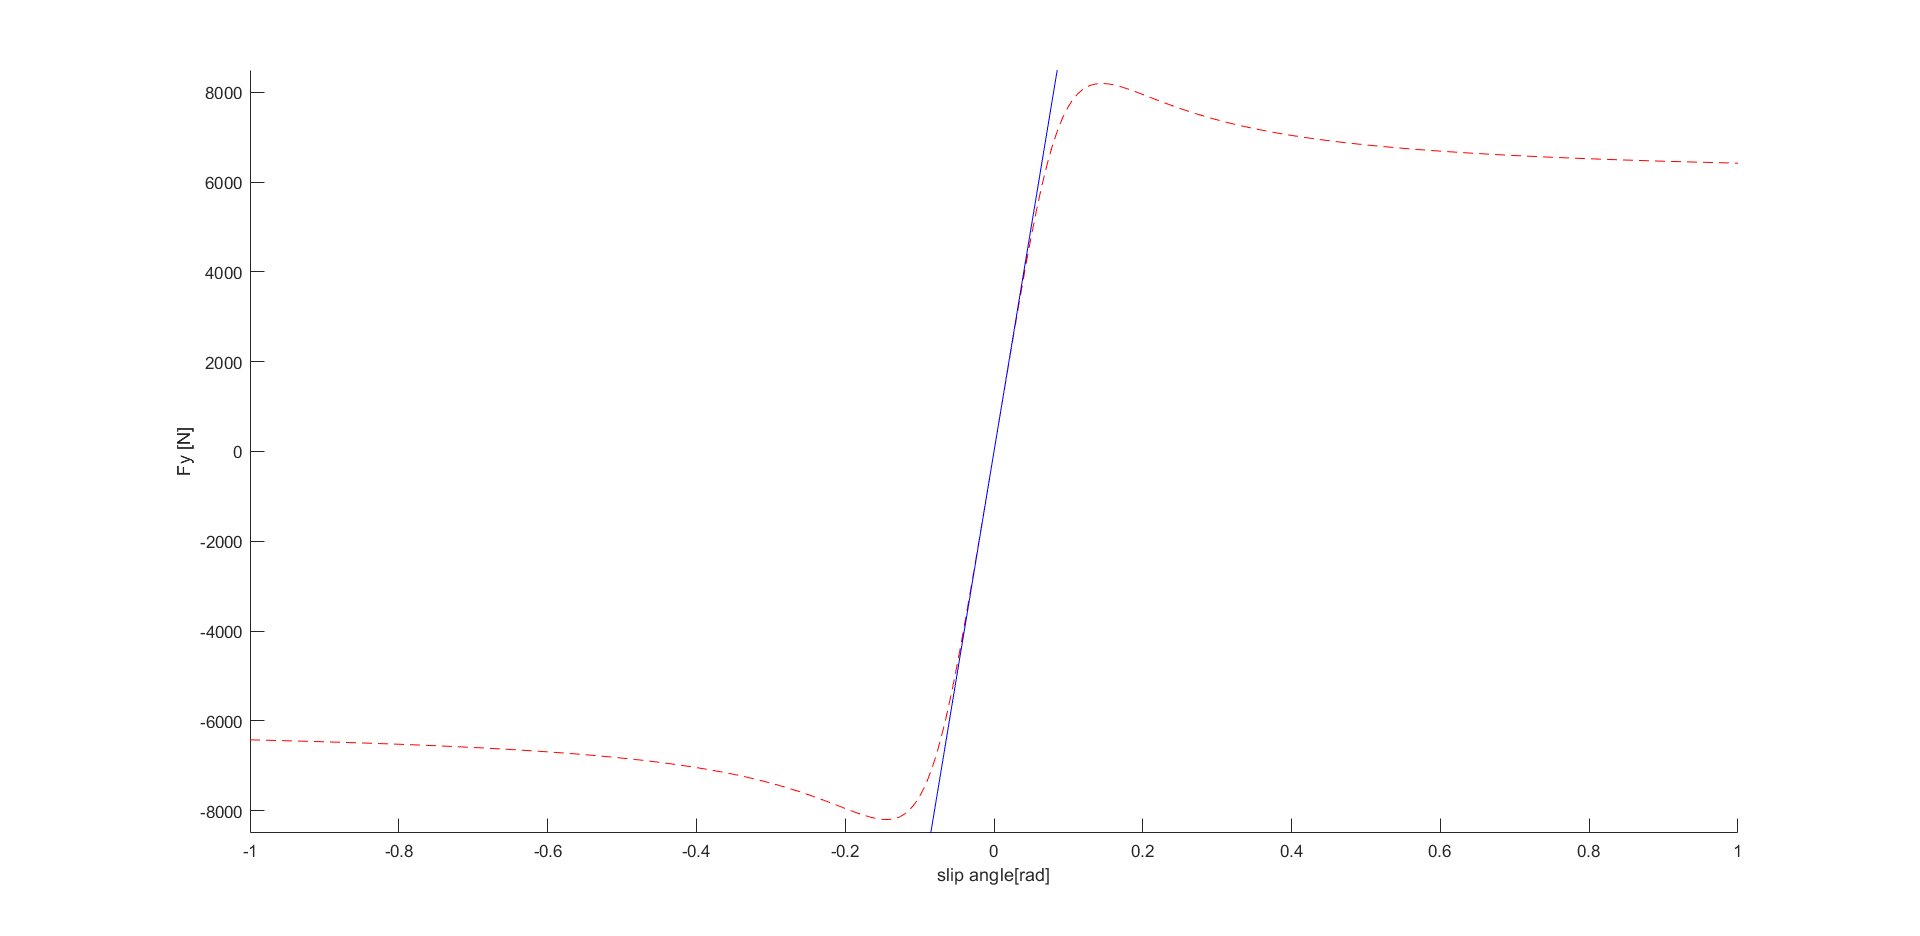
\includegraphics[width=\linewidth]{images/chapter2/Cf.png}
    \caption{Linear vs non-linear modely on front tyre with $C_F = 100000$}
    \label{fig:Cf}
\end{figure}

\begin{figure}[h!]
    \centering
    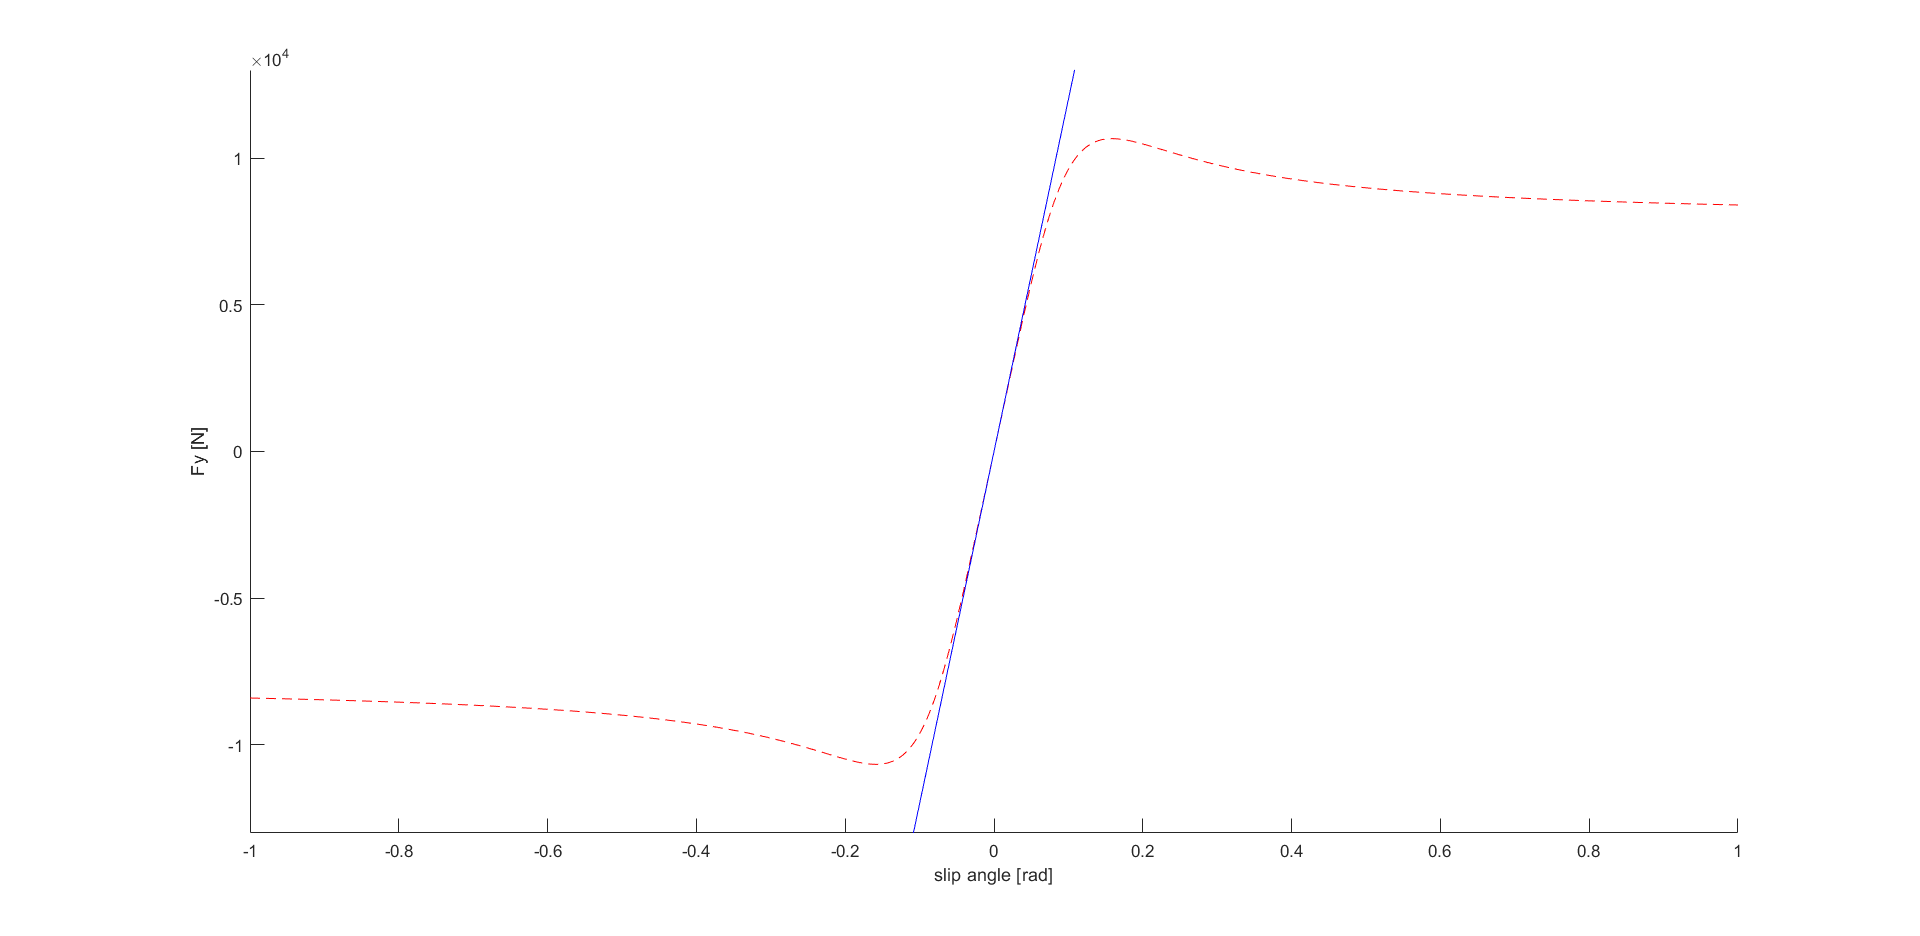
\includegraphics[width=\linewidth]{images/chapter2/Cr.png}
    \caption{Linear vs non-linear modely on rear tyre with $C_R = 120000$}
    \label{fig:Cr}
\end{figure}



\section{Longitudinal control}
The goal of the longitudinal controller is to make the vehicle follow a given speed profile. At first, this profile simply denotes the speed the vehicle must have in each point of the predefined trajectory expressed using the curvilinear abscissa. Given that, using the position of the vehicle, the desired speed is calculated by looking up in the profile table searching for the nearest point with respect to the vehicle position; the actual velocity of the vehicle is subtracted to the desired one and this error is fed to a controller that gives to the model the longitudinal force on the rear wheel ($F_{xR}$) in order to minimize this error, and thus obtaining the required velocity. The block scheme is represented in figure \ref{fig:longController_blocks}
\begin{figure}[h!]
    \centering
    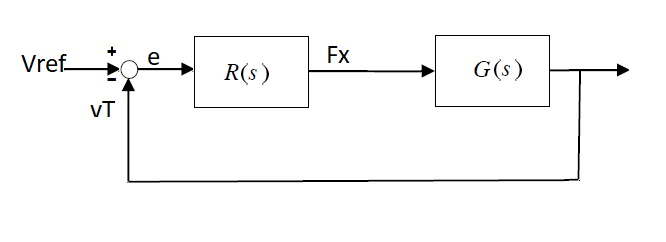
\includegraphics[width=\linewidth]{images/chapter2/longitudinal/blocks.png}
    \caption{Block scheme}
    \label{fig:longController_blocks}
\end{figure}

From the linear model we calculated the transfer function from $F_{xR}$ to the velocity of the vehicle, the plant, and it is
\begin{equation*}
\begin{aligned}
G(s) = \frac{\frac{1}{m_T}}{s}
\end{aligned}
\end{equation*}

The designed controller is of order two and is of the form
\begin{equation*}
\begin{aligned}
R(s) = \frac{k}{s} * \frac{(1 + \frac{s}{2 \pi f_z})^2}{1 + \frac{s}{2 \pi f_p}}
\end{aligned}
\end{equation*}
\\Tuning was done in order to achieve these requirements:
\begin{itemize}
    \item Reject ramp disturbances of velocity profile: to obtain this an integrator $\frac{1}{s}$ was inserted. Thus, also considering the integrator in the transfer function of the plant, the requirement is satisfied
    
    \item Obtain a bandwidth of at least 1 [Hz]
    
    \item Closed loop system stable
\end{itemize}
Tuned parameters are: $f_z = 0.06$ [Hz], $f_p = 0.03$ [Hz] and $k = 5.2$ x $10^3$. The double zeros were chosen to be coincident for tuning simplicity and were added to obtain a raise of the phase margin in order for the system to be stable. The pole at frequency $f_p$ was added to obtain the desired bandwidth and to have a causal regulator.
\\From figures \ref{fig:longController_Gs} and \ref{fig:longController_Ls} we can see the Bode plot of G(s) and of the open loop function L(s) = R(s) G(s)

\begin{figure}[h!]
    \centering
    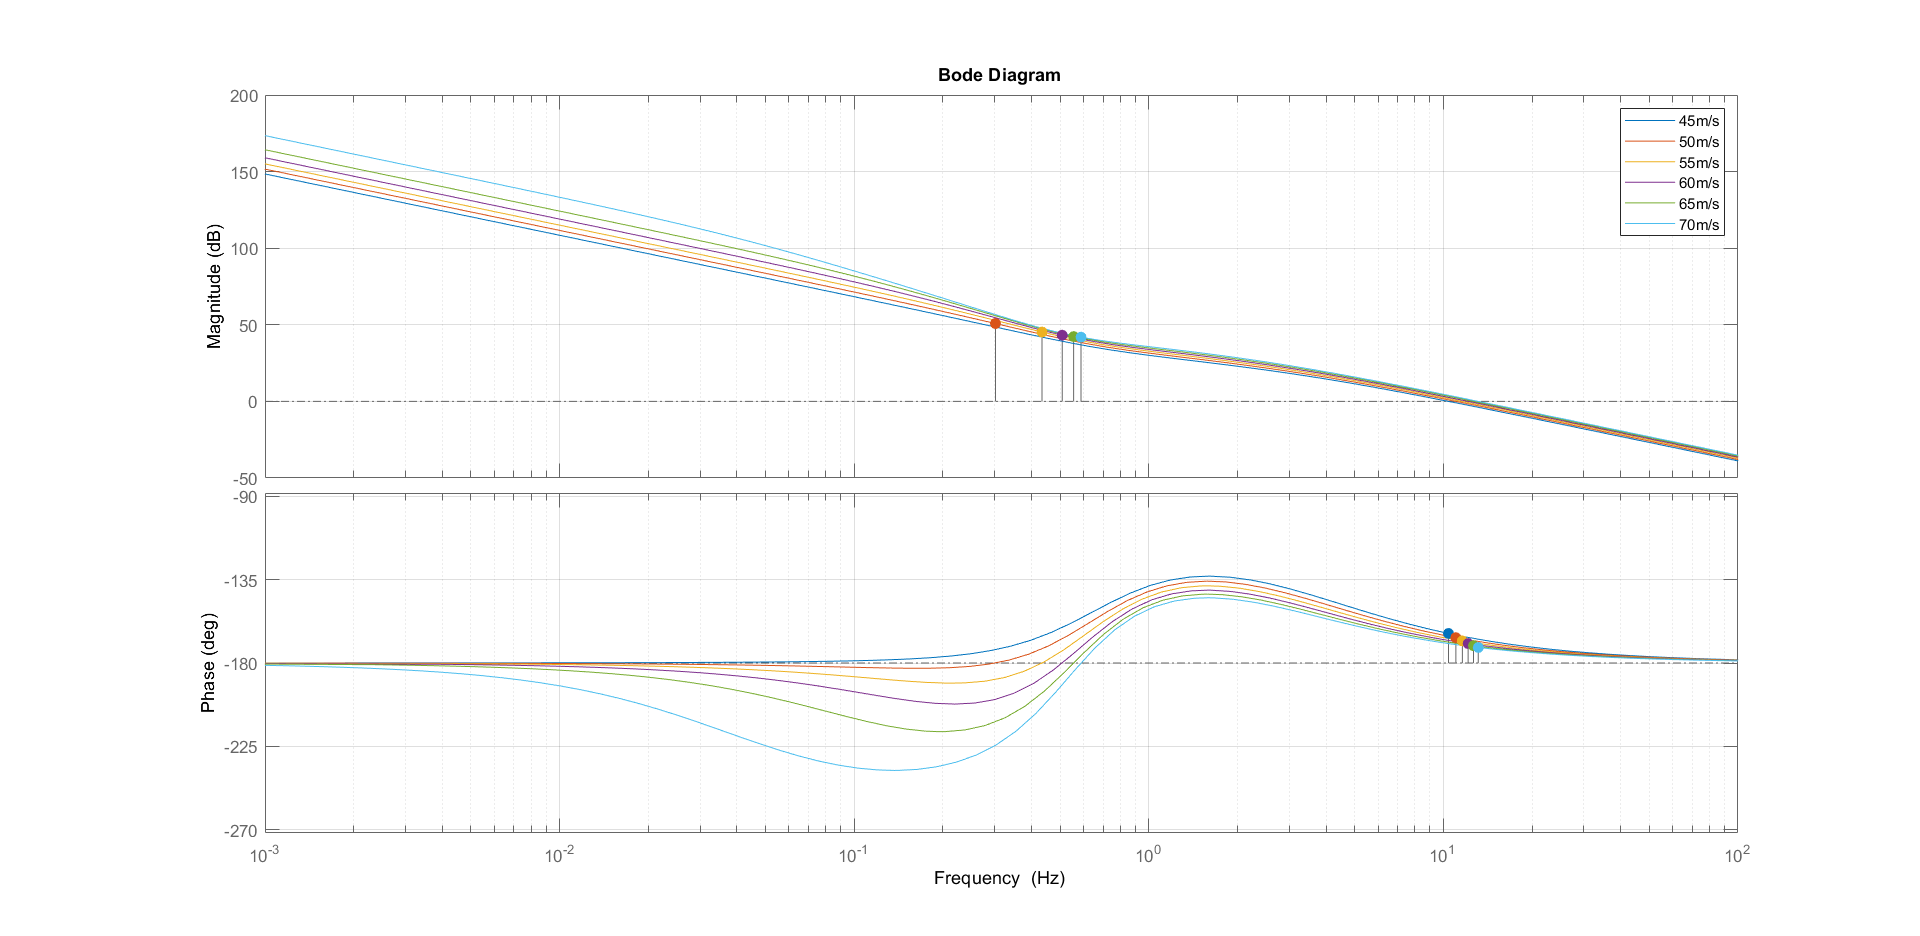
\includegraphics[width=\linewidth]{images/chapter2/longitudinal/Gs.png}
    \caption{Bode diagram of the plant G(s)}
    \label{fig:longController_Gs}
\end{figure}

\begin{figure}[h!]
    \centering
    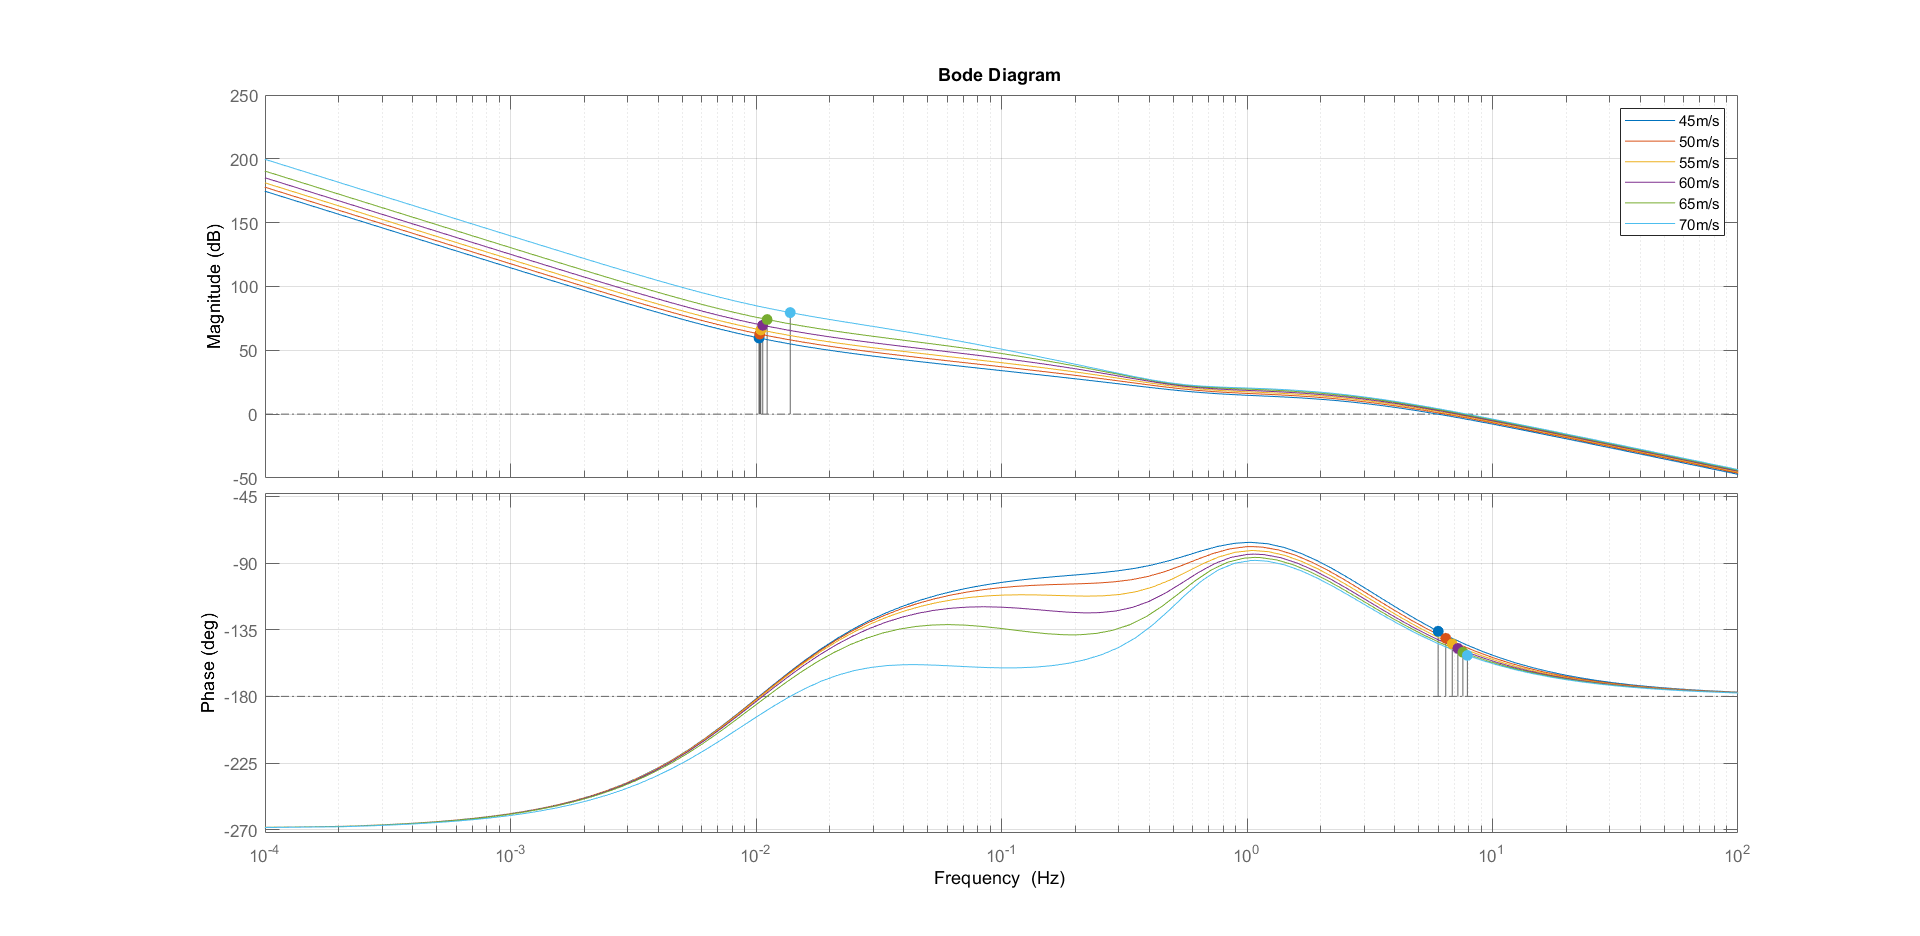
\includegraphics[width=\linewidth]{images/chapter2/longitudinal/Ls.png}
    \caption{Bode diagram of the open loop function L(s) vs the plant G(s)}
    \label{fig:longController_Ls}
\end{figure}

Moreover from figures \ref{fig:longController_Ls} we can see that for the Bode criterion the closed loop system is stable since the phase margin is 86 [deg] $>$ 0, and that the bandwidth is 1.44 [Hz]
\\\\From figures \ref{fig:longController_sinwave} and \ref{fig:longController_vref} we can see the response of the system with the designed regulator to a sinusoidal wave and to the generated speed profile to follow during the trajectory. As can be seen, the reference velocity is well followed. 

\begin{figure}[h!]
    \centering
    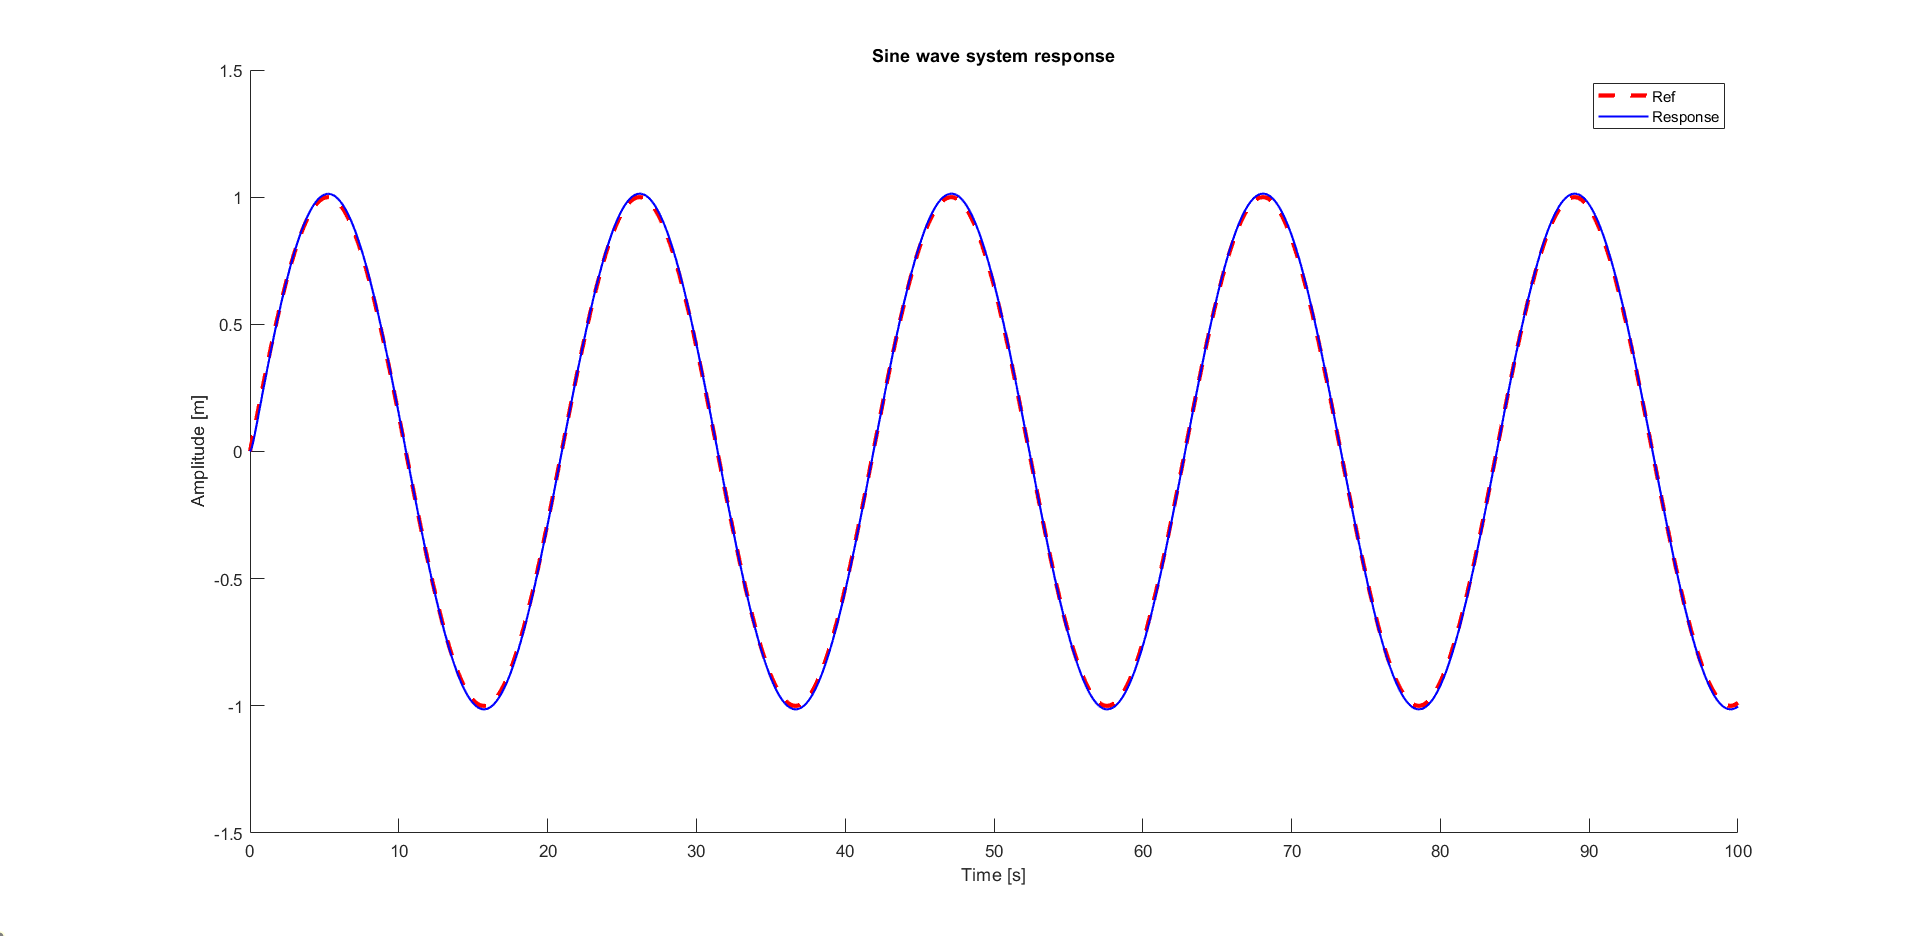
\includegraphics[width=\linewidth]{images/chapter2/longitudinal/SineWave_response.png}
    \caption{System response to sin wave}
    \label{fig:longController_sinwave}
\end{figure}

\begin{figure}[h!]
    \centering
    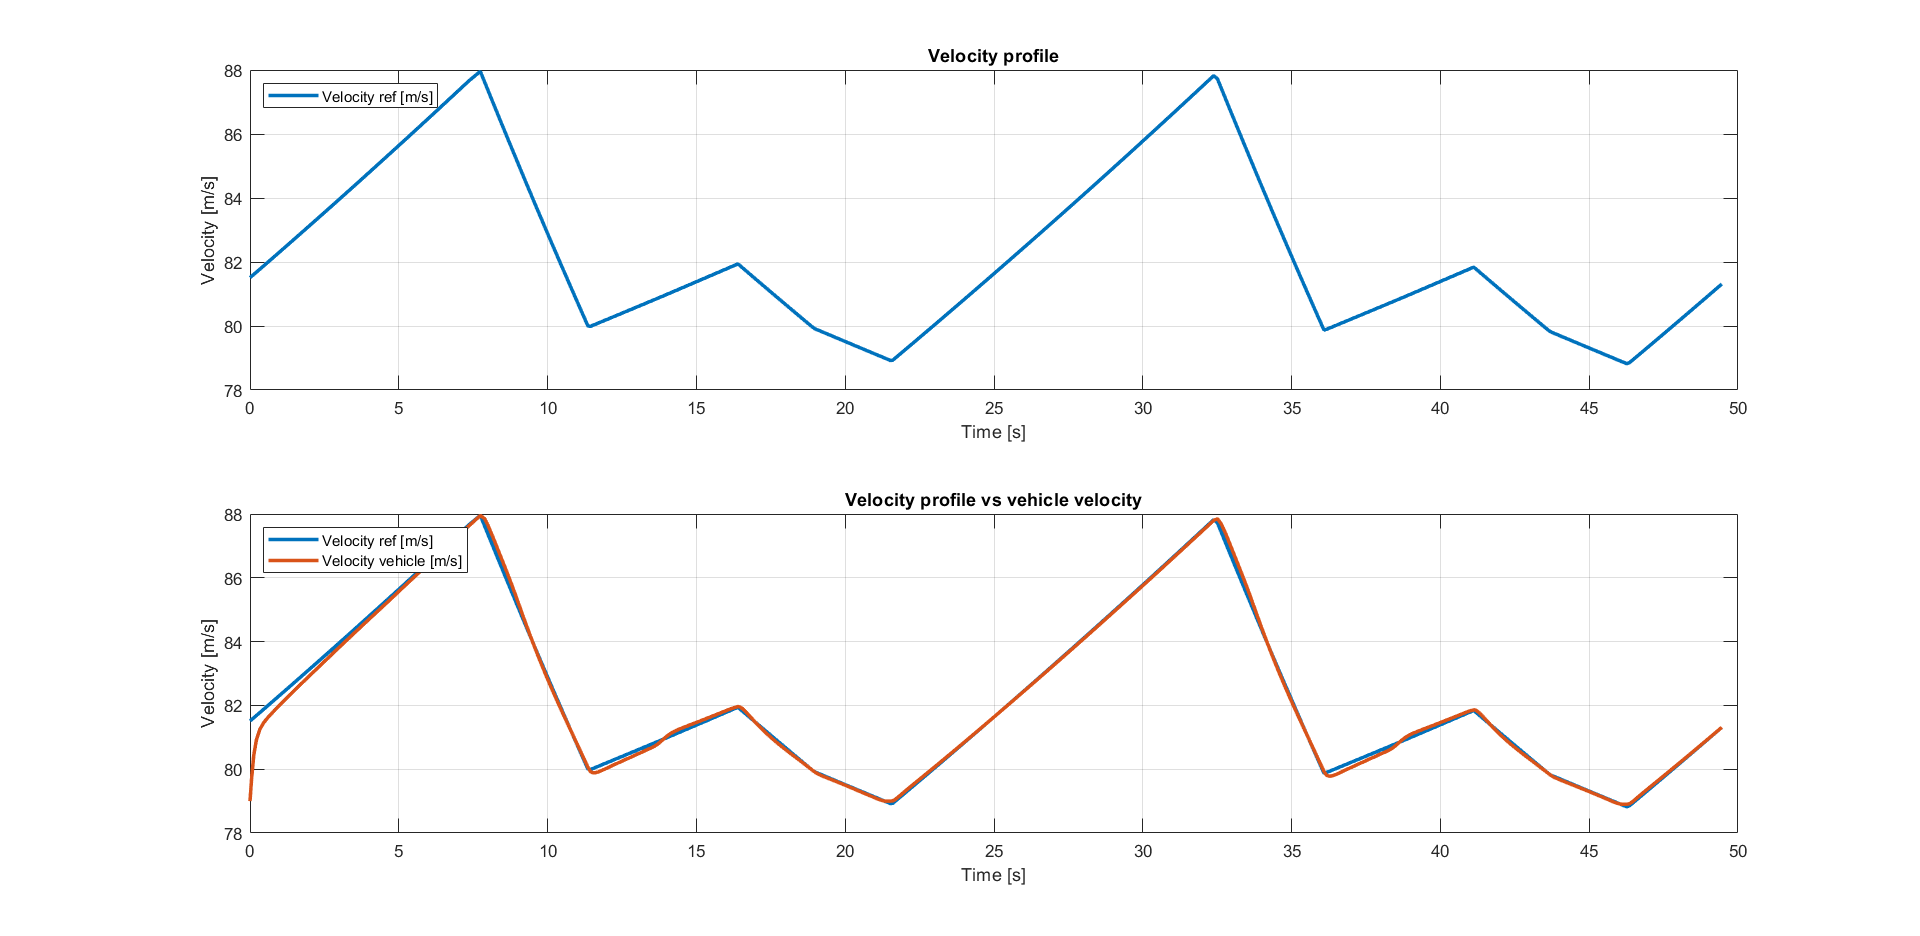
\includegraphics[width=\linewidth]{images/chapter2/longitudinal/responseRef.png}
    \caption{System response to speed profile}
    \label{fig:longController_vref}
\end{figure}


\section{Lateral control}
The goal of the lateral controller is to give to the vehicle the correct steering angle in order to minimize the lateral error with respect to the predefined trajectory. The trajectory is generated, as for the speed profile, as a function of the curvilinear abscissa, meaning that for each value of it, desired x, y and yaw angle are expressed. Anyway, the lateral error is not computed referring to the centre of mass of the vehicle but based on a lookahead distance. Thus, the controller first calculates the coordinates of the virtual point which is an approximation of where the vehicle will be in the next instants. The virtual point is computed using the lookahead distance and the current yaw angle, then it checks the distance between the nearest point on the trajectory and this virtual point and feeds the regulator with this error. Concerning the lookahead distance, we choose it to be dynamic and having a modulus equal to the longitudinal speed of the vehicle scaled by a constant of with value 1/2. 
\\To design the lateral controller a further simplification has been considered: the longitudinal dynamics was neglected. Moreover a change of state has been done in order to have as resulting states just the lateral velocity $V_y$ and the yaw rate $\dot{\psi}$. As we already said, since the longitudinal velocity $V_x$ is considered constant because it varies with a much slower dynamic with respect to the lateral one and because the linearization is done assuming we are traversing a straight path with a constant speed, we have that $v_T$ = $v_{T0}$ = $V_x$

\begin{equation}
\begin{aligned}
V_y = v_{T0} sin(\beta)\\\\
\text{Using the small angle assumption of the linear model}\\\\
V_y = v_{T0} \beta\\\\
\text{so: }\\\\
\frac{V_y}{v_{T0}} = \beta\\\\
\end{aligned}
\end{equation}

We obtain

\begin{equation}
\begin{aligned}
\dot{V_y} = -\frac{C_F + C_R}{m_T V_x} V_y + (\frac{C_R l_R - C_F l_F}{m_T V_x} - V_x) \dot{\psi} + \frac{C_F}{m_T} \delta\\
\ddot{\psi} = \frac{C_R l_R - C_F l_F}{I_T V_x} V_y - \frac{C_F l_F^2 - C_R l_R^2}{I_T V_x} \dot{\psi} + \frac{C_F l_F}{I_T} \delta\\\\
\end{aligned}    
\end{equation}

To this model two states were added to take into consideration the dynamic of the error. The first state $e_{cg}$ represents the lateral positioning error with respect to the center of gravity; the second state $\Delta\psi$ is the heading angle error, representing the difference between the desired yaw angle and the actual one. The reference path is described by the coordinates $X_t$, $Y_t$ and the curvature $\rho_t$. $V_t$ is the speed at the reference point.

\begin{equation}
\begin{aligned}
\dot{e_{cg}} = V_y cos(\Delta\psi) + V_x sin(\Delta\psi)\\
\dot{\Delta\psi} = \dot{\psi} - \rho_t V_t\\\\
\end{aligned}    
\end{equation}

\begin{figure}[h!]
    \centering
    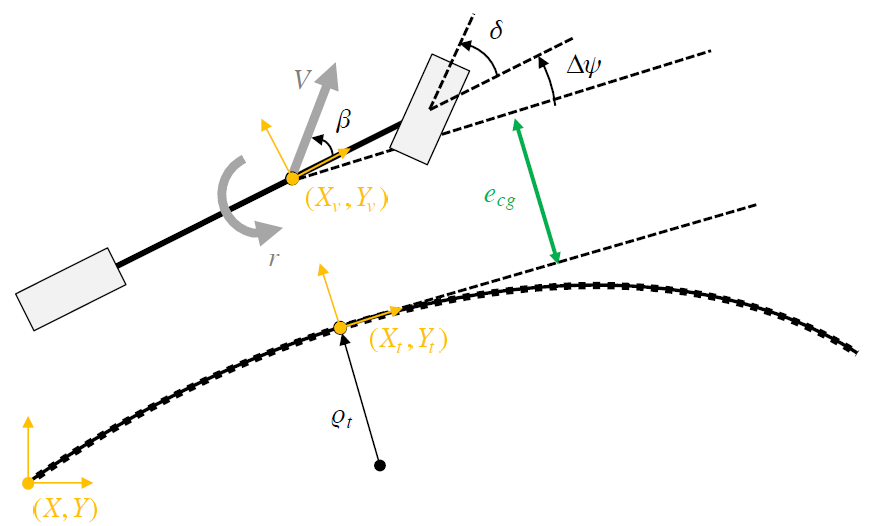
\includegraphics[width=\linewidth]{images/chapter2/lateral/ext.png}
    \caption{Lateral positioning error and heading angle error}
    \label{fig:latController_ext}
\end{figure}

Assuming small angles and that the velocity is well tracked we have:
\begin{equation}
\begin{aligned}
\dot{e}_{cg} = V_y + V_x \Delta\psi\\
\dot{\Delta\psi} = \dot{\psi} - \rho_t V_x\\\\
\end{aligned}    
\end{equation}

These two equations are added to the previous state space model. The output of the system would simply be $e_{cg}$ but since we decided to use the lookahead error we have as output

\begin{equation}
\begin{aligned}
y = e_{la} = e_{cg} + d_{la} \Delta\psi
\end{aligned}    
\end{equation}

Where $d_{la}$ is the chosen distance of lookahead, set to $V_x/k$ where k is 2 $[s^{-1}]$ so to take the distance in which will 1/2 seconds later, as already said.
\\In matrix notation
\begin{equation}
\begin{aligned}
\dot{x} = A x + B u \\
\dot{x} = 
\begin{bmatrix}
    -\frac{C_F + C_R}{m_T V_x} & \frac{C_R l_R - C_F l_F}{m_T V_x} - V_x & 0 & 0\\\\
    \frac{C_R l_R - C_F l_F}{I_T V_x} & - \frac{C_F l_F^2 - C_R l_R^2}{I_T V_x}  & 0 & 0 \\\\
    1 & 0 & 0 & V_x \\\\
    0 & 1 & 0 & 0
\end{bmatrix}
\begin{bmatrix}
    V_y \\
    \dot{\psi}\\
    e_{cg}\\
    \Delta\psi\\
\end{bmatrix}
+
\begin{bmatrix}
    \frac{C_F}{m_T} & 0\\\\
    \frac{C_F l_F}{I_T} & 0\\\\
    0 & 0\\\\
    0 & -V_x
\end{bmatrix}
\begin{bmatrix}
    \delta\\
    \rho
\end{bmatrix}\\\\
y = C x + D u; D = 0\\
y = 
\begin{bmatrix}
    0 & 0 & 1 & d_{la}
\end{bmatrix}
\begin{bmatrix}
    V_y \\
    \dot{\psi}\\
    e_{cg}\\
    \Delta\psi\\
\end{bmatrix}
\end{aligned}
\end{equation}
This is the model used to design the regulator, thus we computed the transfer function between the steering angle $\delta$ and the error $e_{la}$ and it is
\begin{equation}
\begin{aligned}
G_{e\_la}(s) = \frac{C_F V_x}{k s^2} \frac{N(s)}{D(s)}\\\\
N(s) = (l_f m V_x^2 + J_z k V_x)s^2 + \\ + (C_r V_x l_r + C_r l_f V_x + C_r k l_r^2 + C_r k l_f l_r)s + \\ + (C_r k V_x l_r + C_r k l_f V_x)\\\\
D(s) = (J_z V_x^2 m)s^2 + \\ + (C_f J_z V_x + C_r J_z V_x + C_f V_x l_f^2 m + C_r V_x l_r^2 m)s + \\ + (C_f C_r l_f^2 + C_f C_r l_r^2 - C_f V_x^2 l_f m + C_r V_x^2 l_r m + 2 C_f C_r l_f l_r)\\\\\\
\end{aligned}    
\end{equation}

The block scheme of the system is the one in figure \ref{fig:latController_blockscheme1} and as can be seen the curvature can be interpreted as external disturbances, in particular a step disturbance. $G_\rho$ is the transfer function between the curvature and the lookahead error and it is

\begin{equation}
\begin{aligned}
G_{\rho}(s) = -\frac{V_x^2 s + V_x^2 k}{k s^2}\\\\
\end{aligned}    
\end{equation}


\begin{figure}[h!]
    \centering
    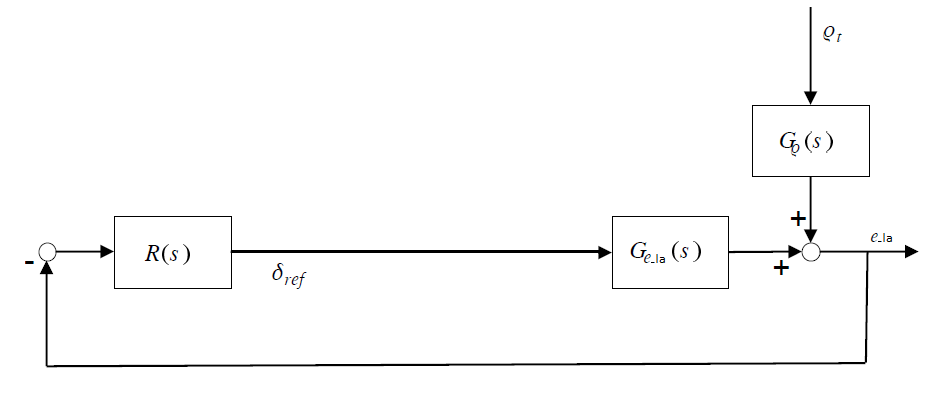
\includegraphics[width=\linewidth]{images/chapter2/lateral/block_scheme_1.png}
    \caption{Block scheme of lateral project}
    \label{fig:latController_blockscheme1}
\end{figure}

The controller was designed to satisfy the following requirements:
\begin{itemize}
    \item Reject step disturbances of curvature: to obtain this an integrator $\frac{1}{s}$ was inserted.
    
    \item Obtain a bandwidth of at least 1 [Hz]
    
    \item Closed loop system stable
\end{itemize}
Thus it is of the form
\begin{equation*}
\begin{aligned}
R(s) = \frac{k}{s} * \frac{(1 + \frac{s}{2 \pi f_z})^2}{1 + \frac{s}{2 \pi f_p}}
\end{aligned}
\end{equation*}
Tuning leads to choose $f_z = 0.01$ [Hz], $f_p = 2$ [Hz] and $k = 2$ x $10^{-4}$.
\\\\Anyways this is not the controller used for the simulator; indeed when testing this one on the non linear model, we came to the conclusion that another integrator was needed to overwhelm non linearity condition. Thus the pole at 2 Hz was removed and another integrator was inserted. \\The final regulator structure is:
\begin{equation*}
\begin{aligned}
R(s) = \frac{k}{s^2} * (1 + \frac{s}{2 \pi f_z})^2
\end{aligned}
\end{equation*}
Tuning leads to choose $f_z = 0.01$ [Hz] and $k = 1.2$ x $10^{-4}$. Different operating points have been chosen, and as can be seen there's not a lot of change in bandwidth to lead us to use a rescheduling coefficient. Figures \ref{fig:latController_Gs} and \ref{fig:latController_Ls} are the Bode diagram of the plant G(s) and of the open loop function L(s) at different velocities from which can be seen that the closed loop system is stable since the phase margin is 40 [deg] $>$ 0 and that satisfies the requirements; moreover the system step response is represented in figure \ref{fig:latController_stepResp}. 

\begin{figure}[h!]
    \centering
    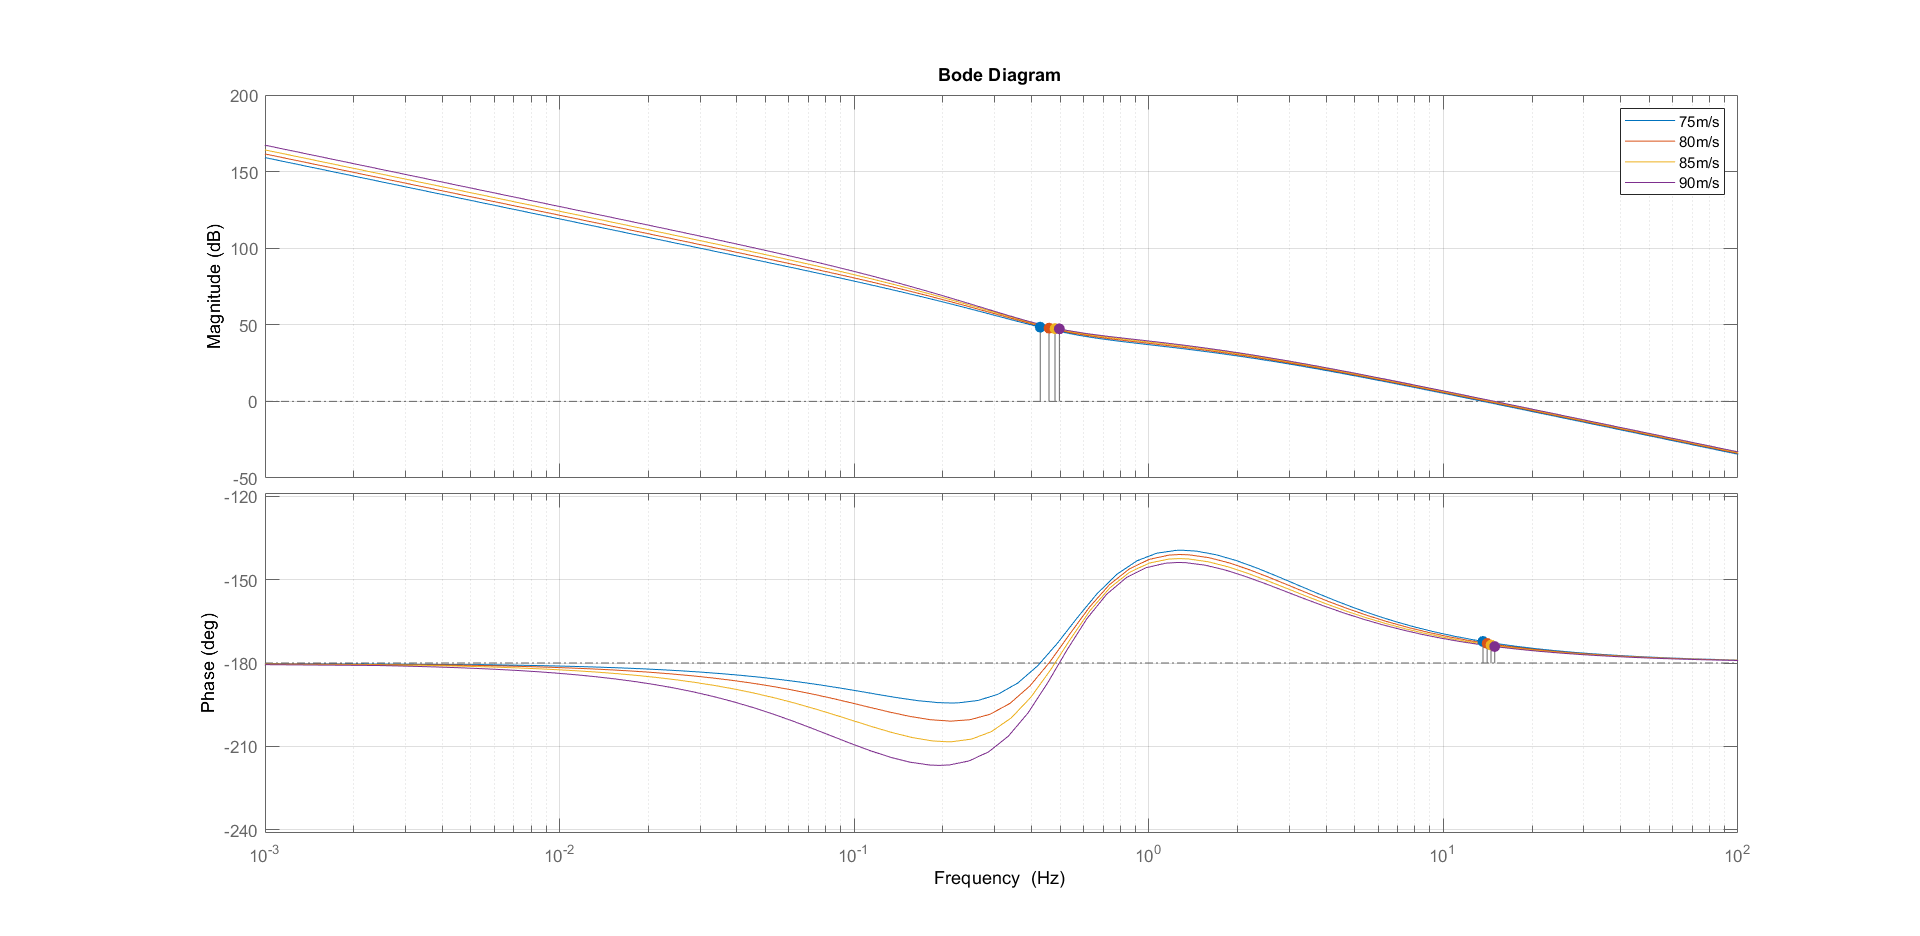
\includegraphics[width=\linewidth]{images/chapter2/lateral/Gs_80.png}
    \caption{Plant G(s), transfer function from $\delta$ to $e_{la}$ at different velocities}
    \label{fig:latController_Gs}
\end{figure}

\begin{figure}[h!]
    \centering
    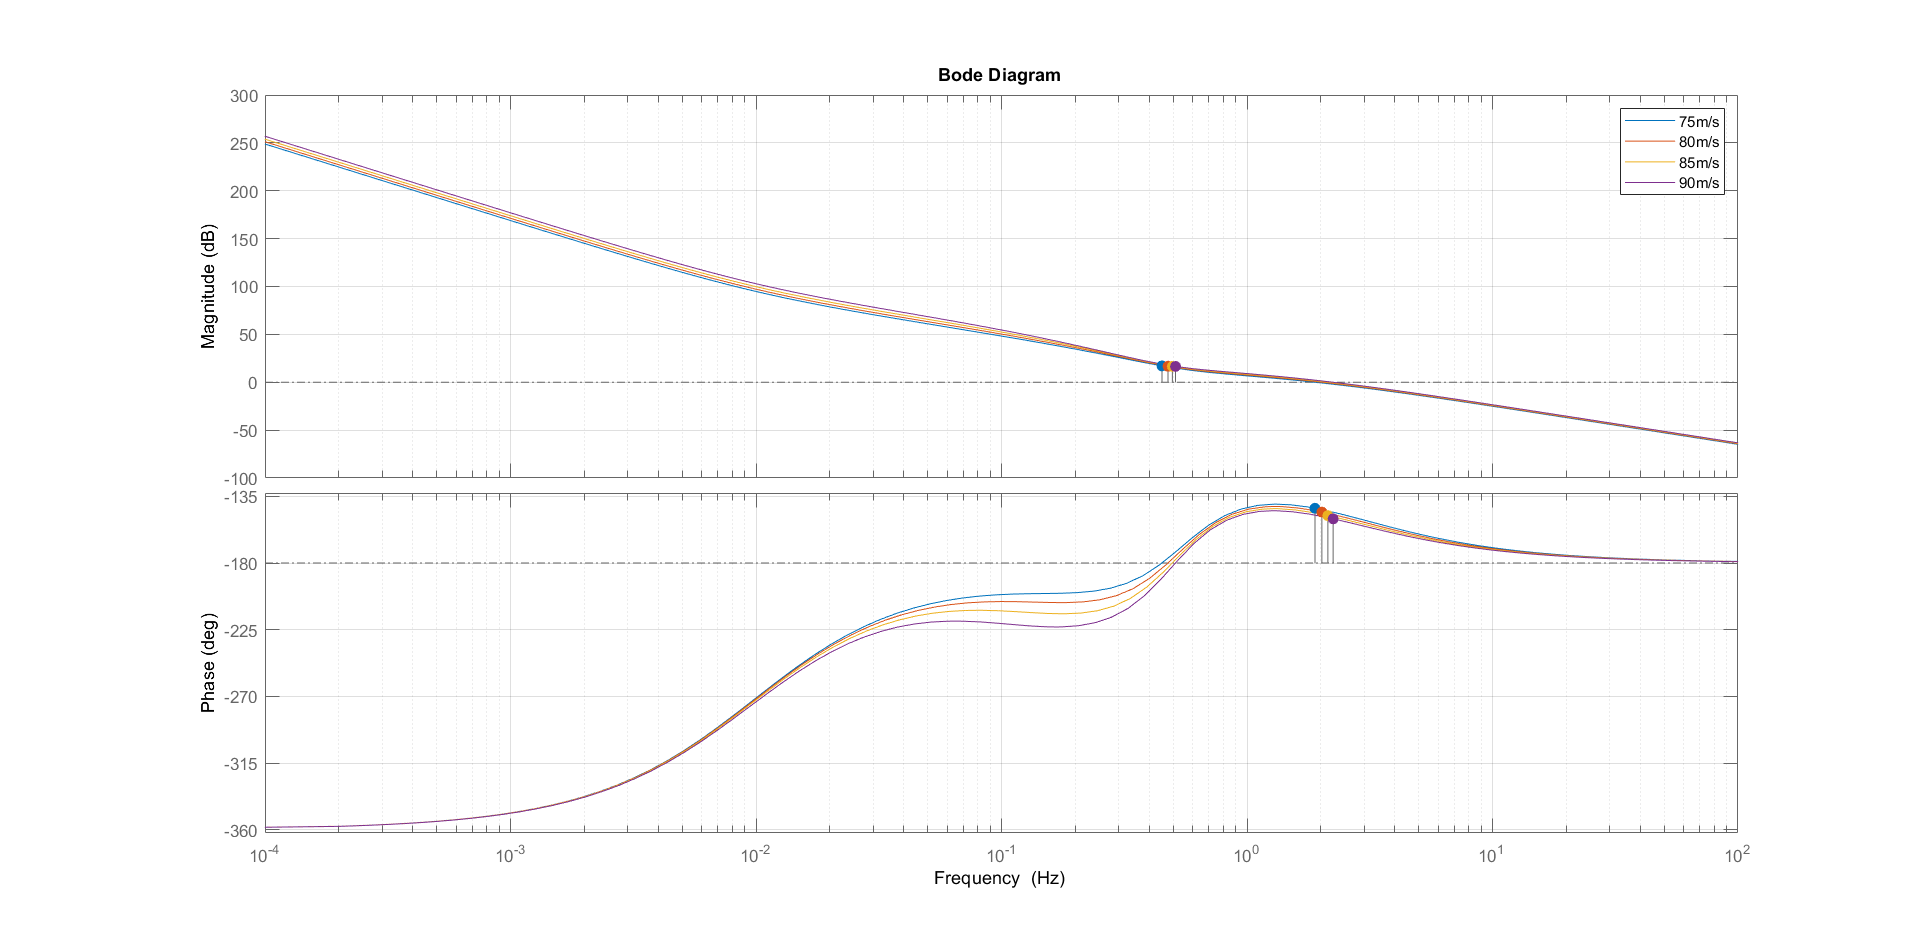
\includegraphics[width=\linewidth]{images/chapter2/lateral/Ls_80.png}
    \caption{Open loop function L(s) at different velocities}
    \label{fig:latController_Ls}
\end{figure}

\begin{figure}[h!]
    \centering
    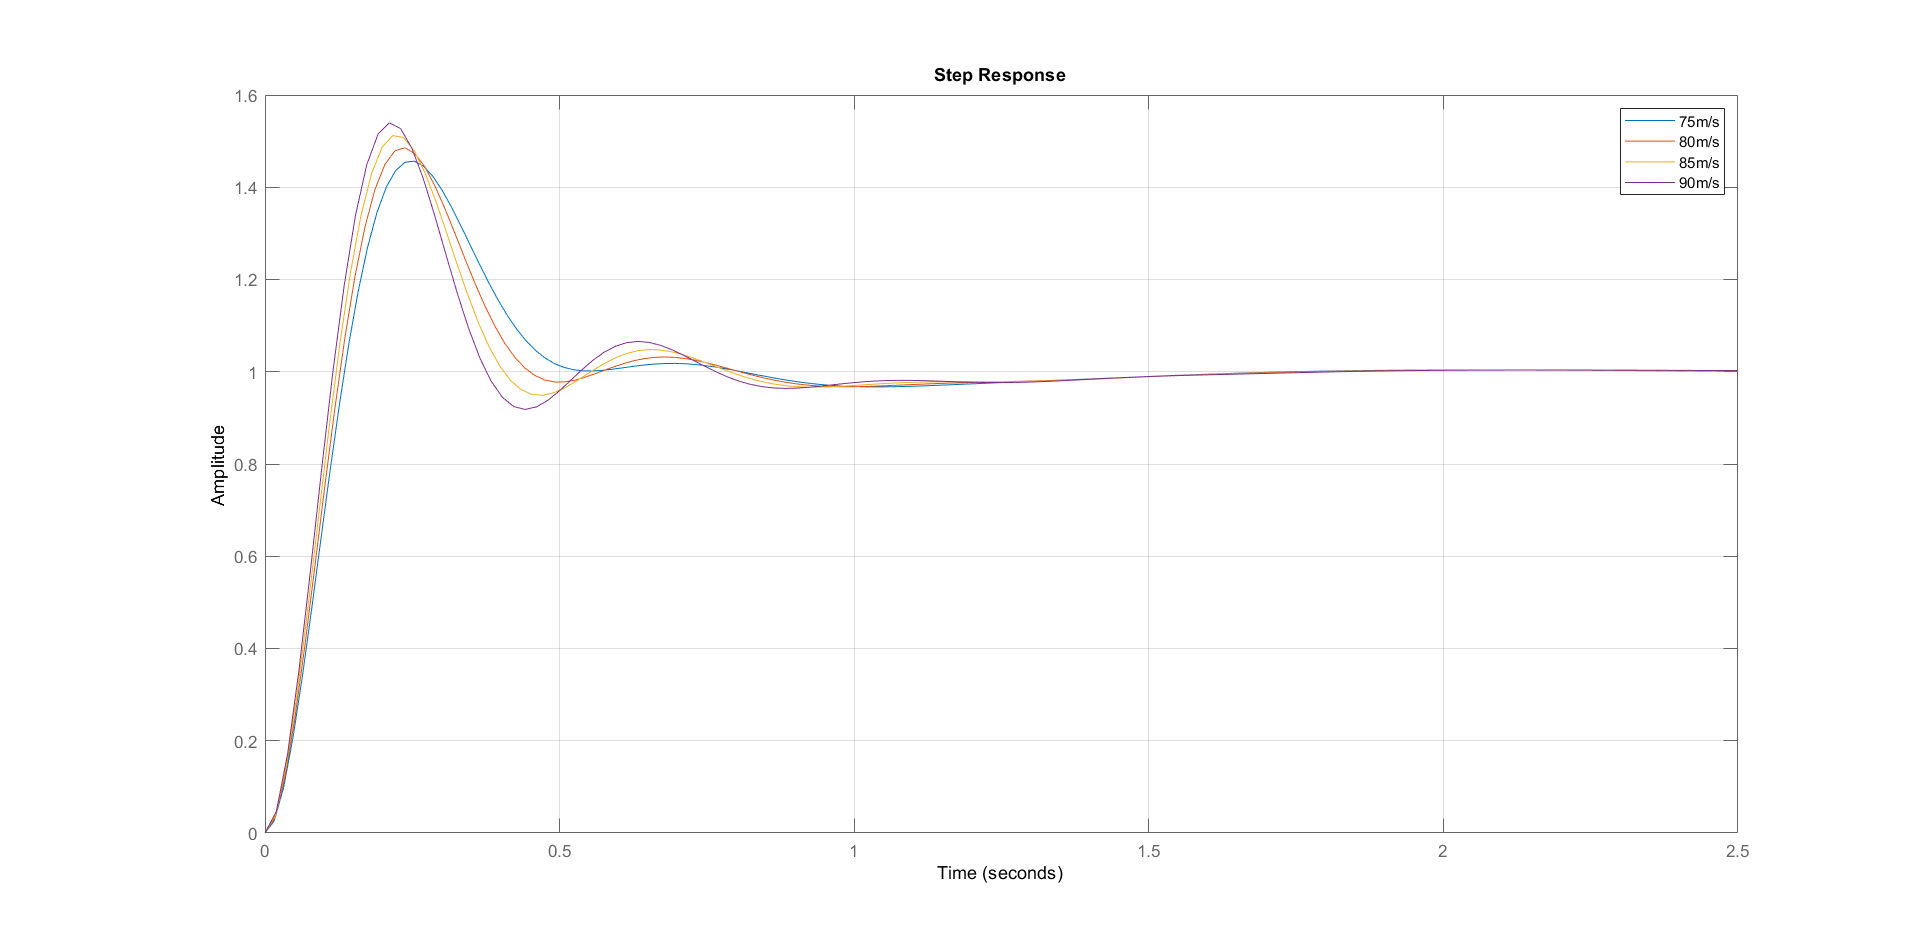
\includegraphics[width=\linewidth]{images/chapter2/lateral/step_resp_80.png}
    \caption{Step response of the system at different velocities}
    \label{fig:latController_stepResp}
\end{figure}

Finally, an open loop component was added, figure \ref{fig:latController_blockscheme2}. It directly acts on the steering angle to compensate curvature error since it is known and acts as disturbance. The main idea is that the curvature disturbance is exploited to anticipate the regulator and to directly give the compensating steering command. Designing it simply, we add it as a gain: 

\begin{equation*}
\begin{aligned}
C(s) = C = - G_{e\_la}(0)^{-1} G_\rho(0) = \\ \frac{m V_x^2 (C_R l_R - C_F l_F) + C_F C_R (l_F+l_R)^2}{C_F C_R (l_F + l_R)}
\end{aligned}
\end{equation*}

\begin{figure}[h!]
    \centering
    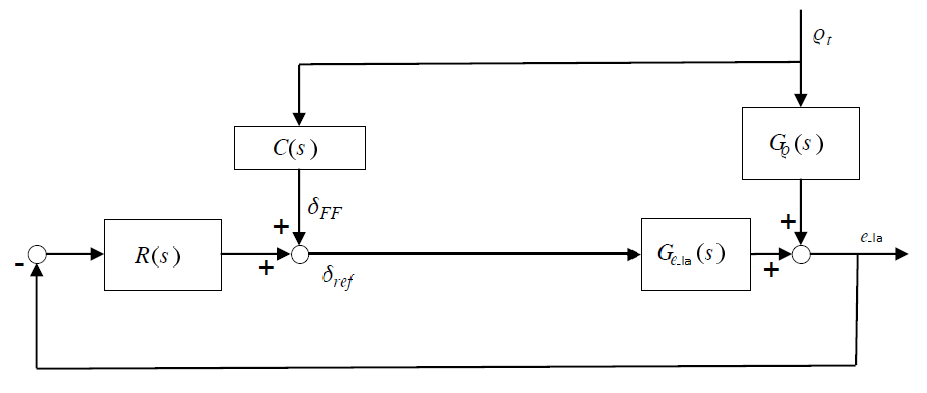
\includegraphics[width=\linewidth]{images/chapter2/lateral/block_scheme_2.png}
    \caption{Final block scheme of lateral project with feed forward compensation}
    \label{fig:latController_blockscheme2}
\end{figure}

\section{Simulation 8 - Lap of the track}
Once designed, both controllers were tested in a first lap simulation on the non linear model in Simulink, focusing on the correctness of the speed profile and in the trajectory tracking focusing on the value of the lateral error with respect to the center of gravity. For completeness, also the followed trajectory, the lateral error on lookahead and the controller steering angle $\delta$ are reported. From what can be seen from those simulations, the controllers work well in the non linear settings of our model, since the speed profile is very well followed despite of the high velocities and the lateral error on center of gravity is in absolute value less then 0.8 [m] = 80 [cm]. Lap time is around 50 [s].

\begin{figure}[h!]
    \centering
    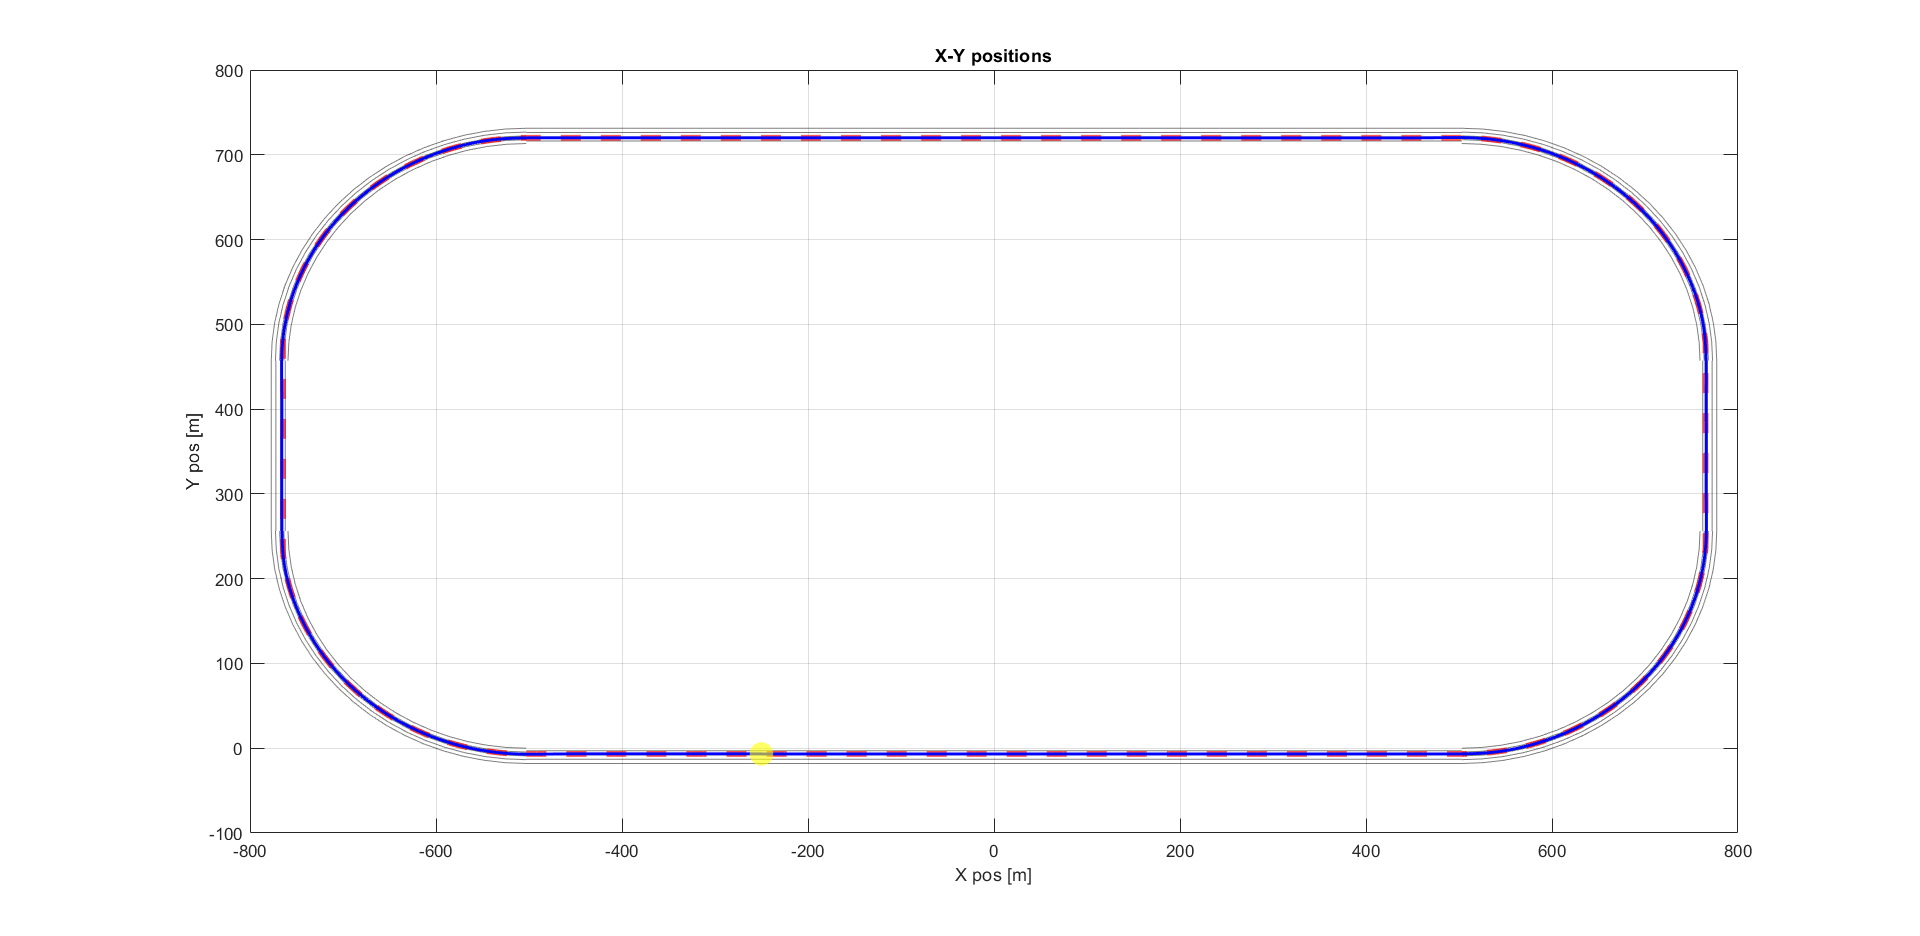
\includegraphics[width=\linewidth]{images/chapter2/lapsim/trajec.png}
    \caption{Trajectory of the simulation}
    \label{fig:latController_lapsim_trajec}
\end{figure}

\begin{figure}[h!]
    \centering
    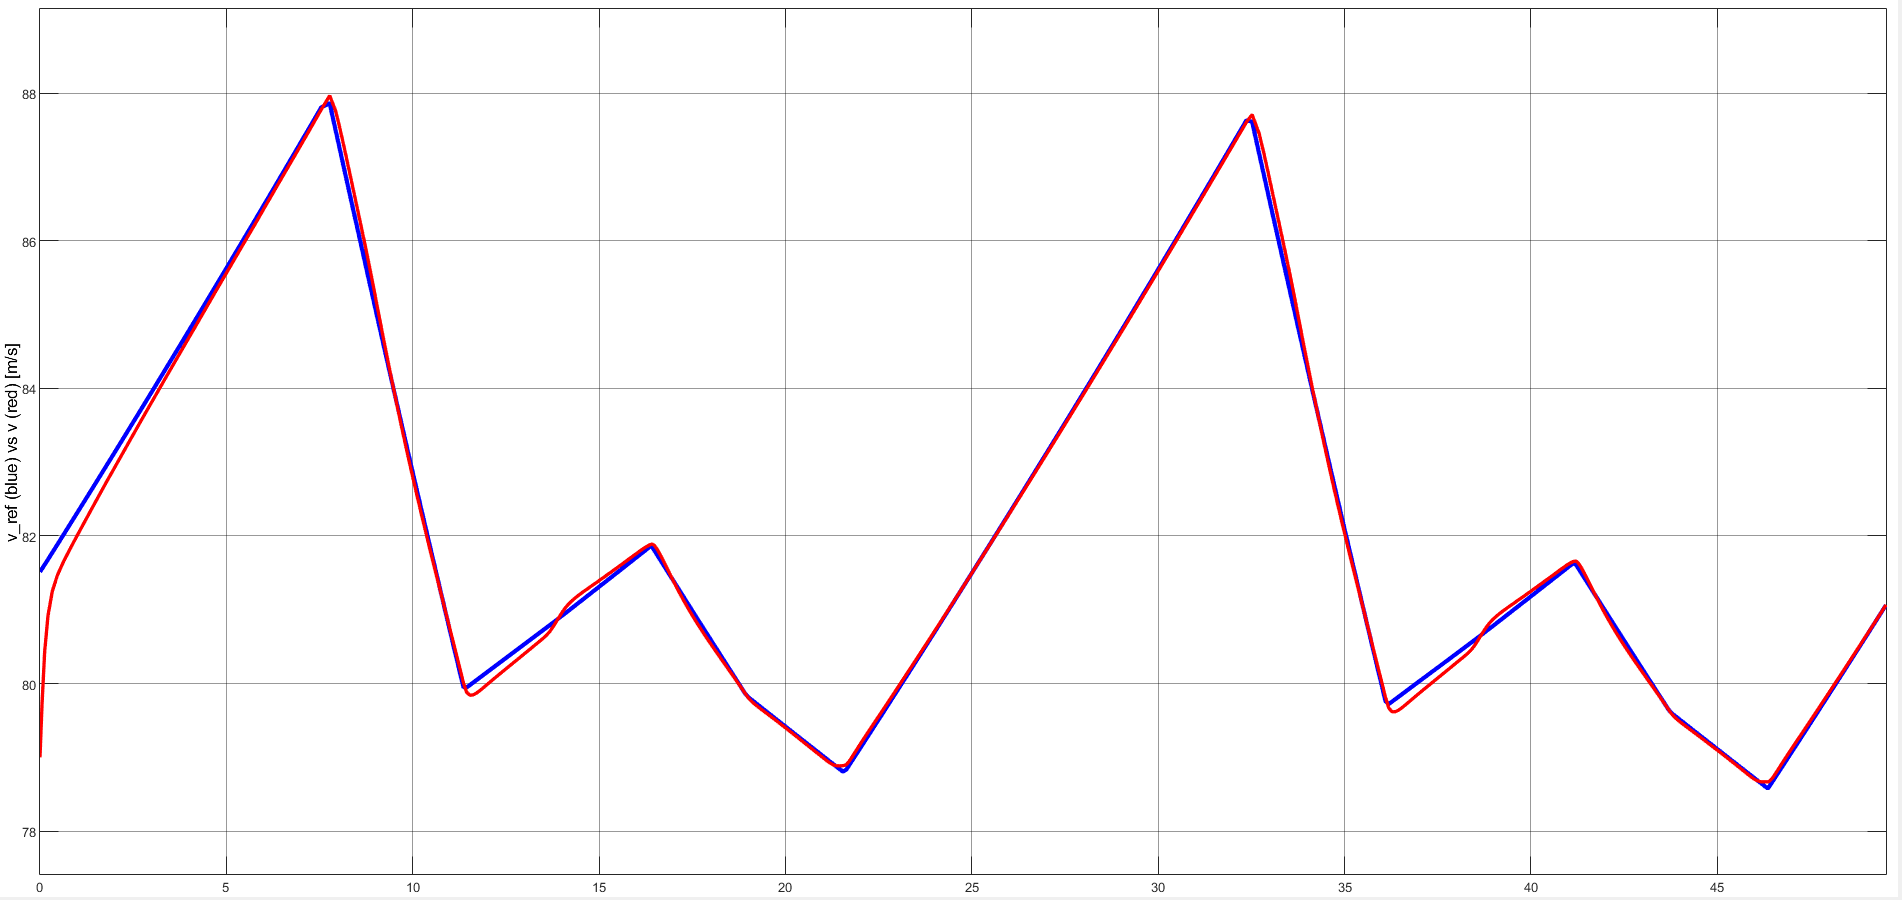
\includegraphics[width=\linewidth]{images/chapter2/lapsim/v.png}
    \caption{Speed profile tracking}
    \label{fig:latController_lapsim_v}
\end{figure}

\begin{figure}[h!]
    \centering
    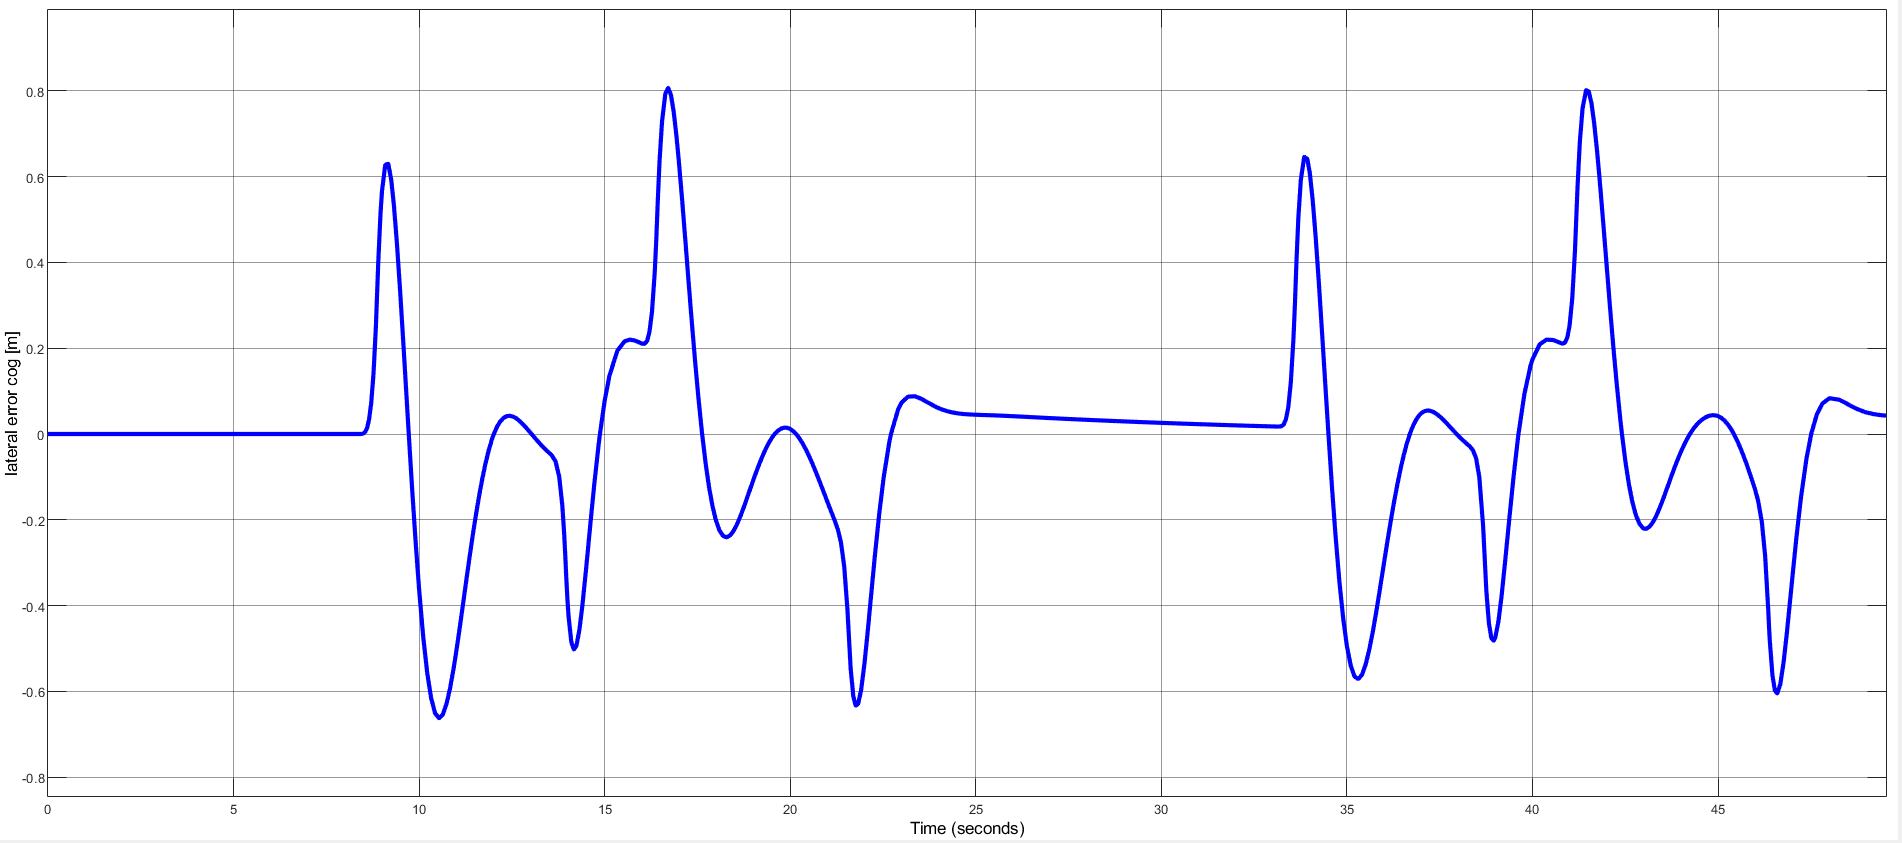
\includegraphics[width=\linewidth]{images/chapter2/lapsim/ecg.png}
    \caption{Lateral error on center of gravity}
    \label{fig:latController_lapsim_ecg}
\end{figure}

\begin{figure}[h!]
    \centering
    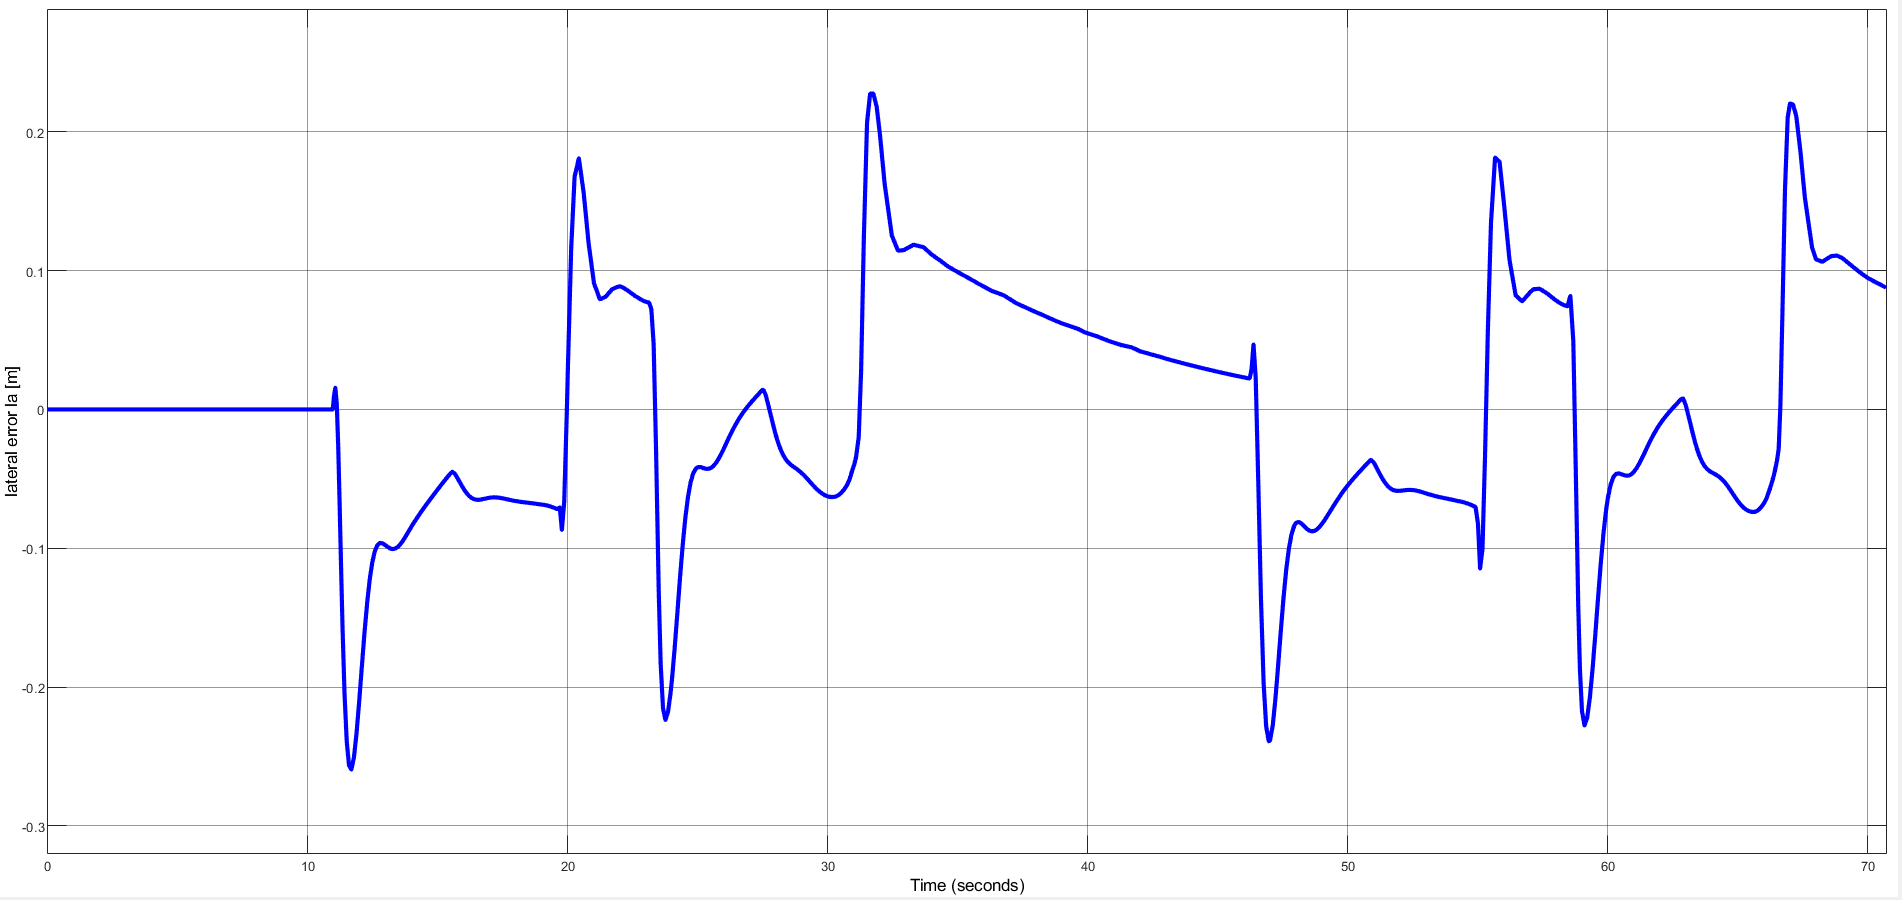
\includegraphics[width=\linewidth]{images/chapter2/lapsim/ela.png}
    \caption{Lateral error on lookahead}
    \label{fig:latController_lapsim_ela}
\end{figure}

\begin{figure}[h!]
    \centering
    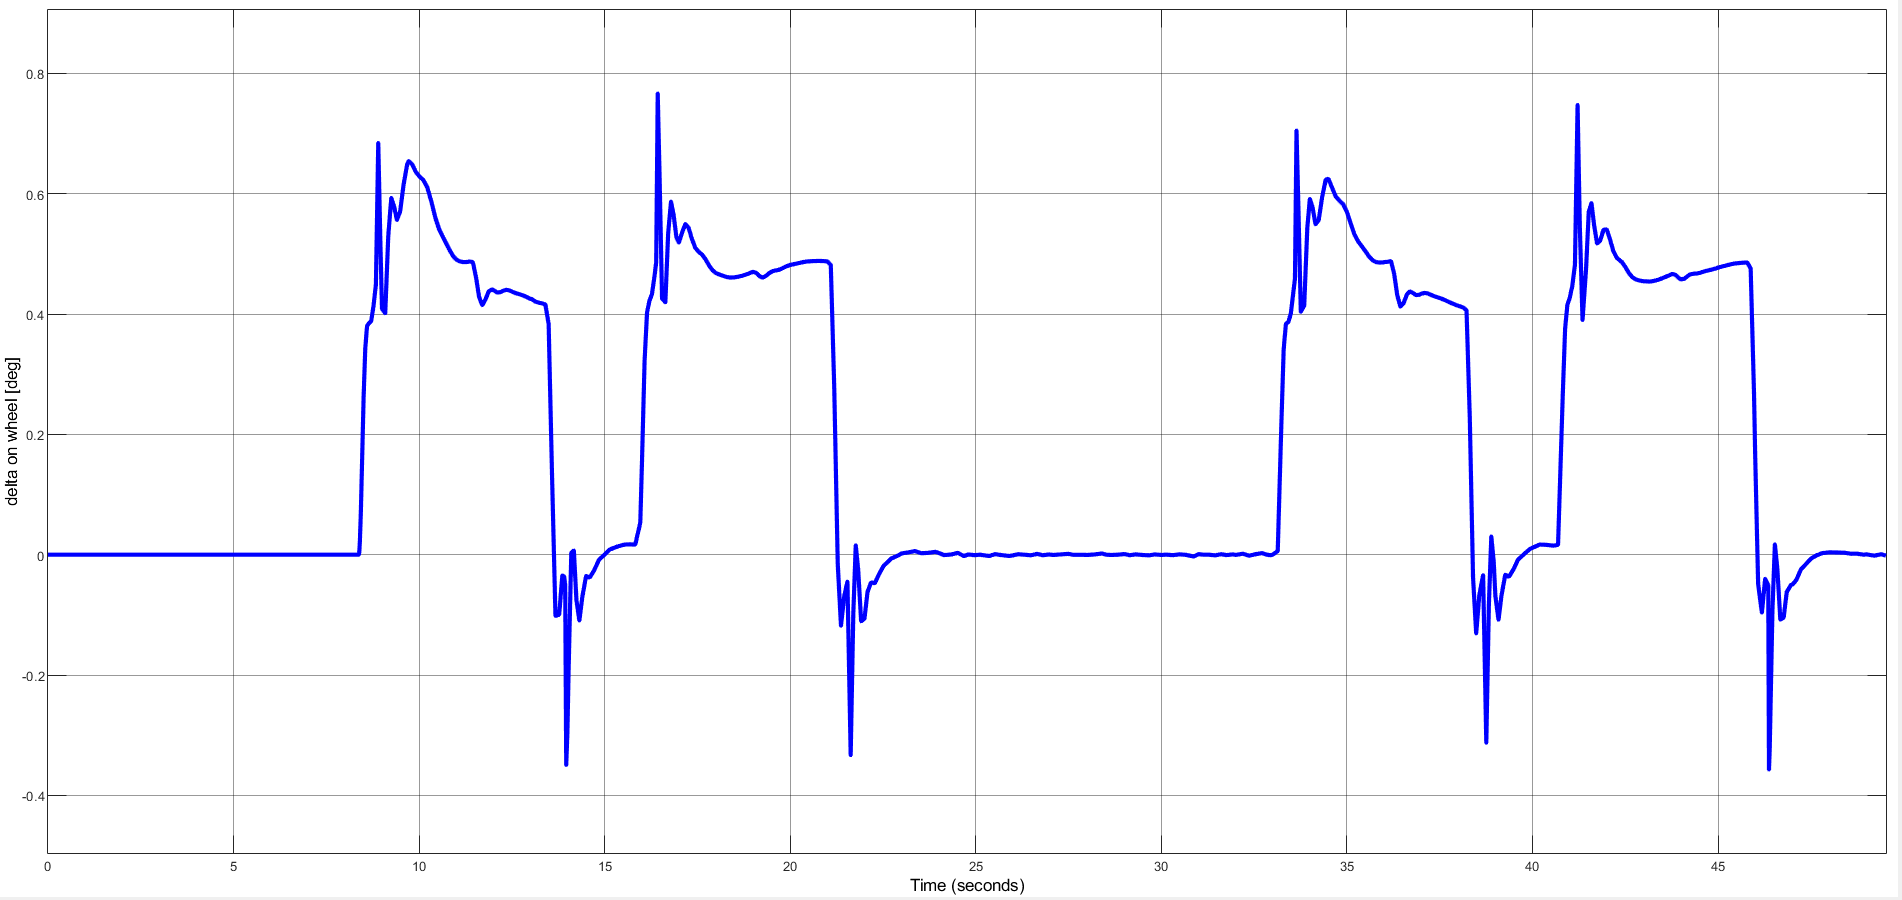
\includegraphics[width=\linewidth]{images/chapter2/lapsim/delta.png}
    \caption{Controlled steering angle}
    \label{fig:latController_lapsim_delta}
\end{figure}

\chapter{Results}
After the model has been implemented and validated, and the controllers have been designed, we run simulations of the race in various conditions to analyze the effect of tyre wear, fuel consumption and slipstreaming. 
\\In particular we defined two different scenarios:
\begin{itemize}
    \item Stress tests: run of laps with a fixed profile at high velocities (80 [m/s] - 88 [m/s]) to analyze how much slipstreaming impacts on performances. 
    \item 20 laps test: the race lasts 20 laps, we analyzed whether and how slipstreaming impacts on different metrics such as fuel consumption and tyre wear
\end{itemize}


\section{Stress tests}
During this test the vehicle tries to follow the fixed speed profile, reported in figure \ref{fig:res_fixedProfile}, for the largest number of laps. The simulations will end for one of this two reasons:
\begin{itemize}
    \item 20 laps are completed
    \item the vehicle cannot handle the velocities anymore and its error with respect to the reference position is larger then 2 meters
\end{itemize}

\begin{figure}[h!]
    \centering
    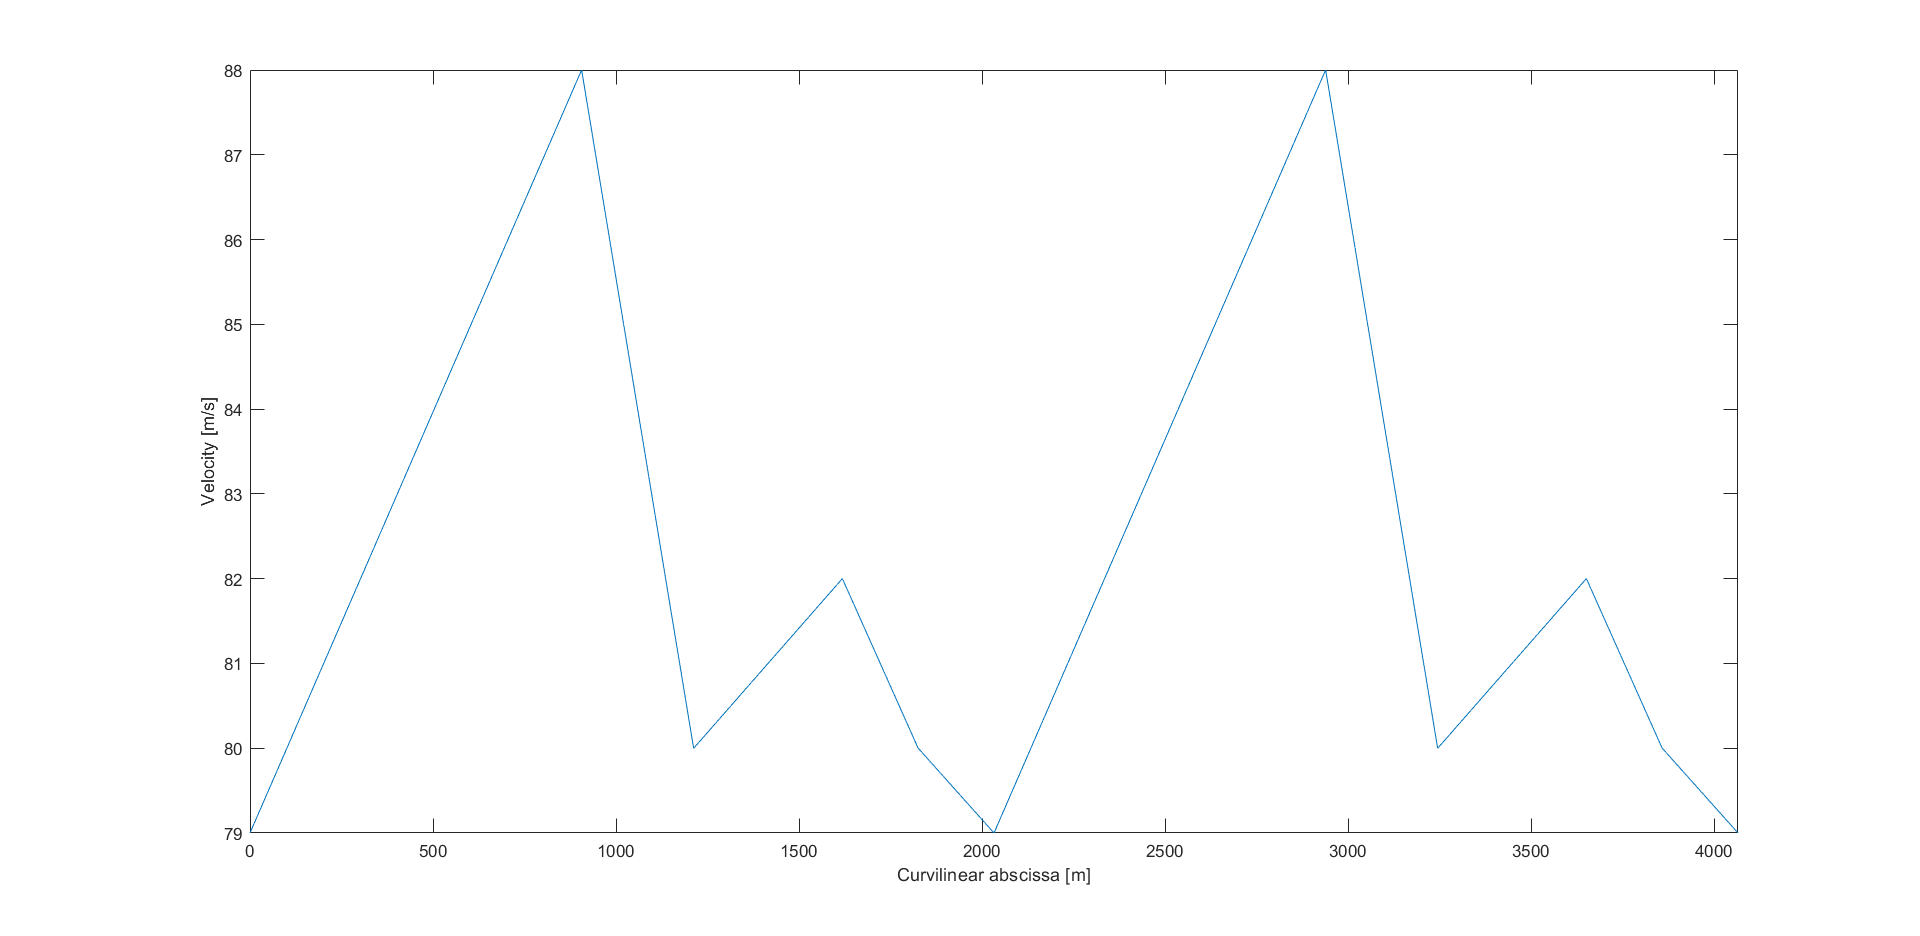
\includegraphics[width=\linewidth]{images/chapter3/velprofile.png}
    \caption{Speed profile function of curvilinear abscissa}
    \label{fig:res_fixedProfile}
\end{figure}

Test is run two times. In the first one the slipstream is off; in the second one slipstream is on during all the simulation time. Although this is not practically realizable, it helps us understand, how much slipstreaming impacts on performances. 
\\Finally the same test is done by spending half of the time without slipstreaming and half of the time slipstreaming. As could be seen from the results, this last simulation leads to very similar conclusions of the "all-time slipstream" one.
\subsection{First run: no slipstreaming}
This test ends since the value of error reached the limit of 2 meters. \\Figure \ref{fig:res_distEllipse_stressNo20} shows the distance of the pair (Fx,Fy) on the friction ellipse with a value 0/1, where 0 represents "far" from the ellipse and "1" represents on the border of the ellipse; IT can be seen that going towards the final seconds the ellipse is going to be saturated. At that time the vehicle had done 12 laps. Also the reduction of the ellipses, that corresponds to a loss in performances since lower forces and thus velocities can be handled, is reported in figures \ref{fig:res_wear_stressNo20}

\begin{figure}[h!]
    \centering
    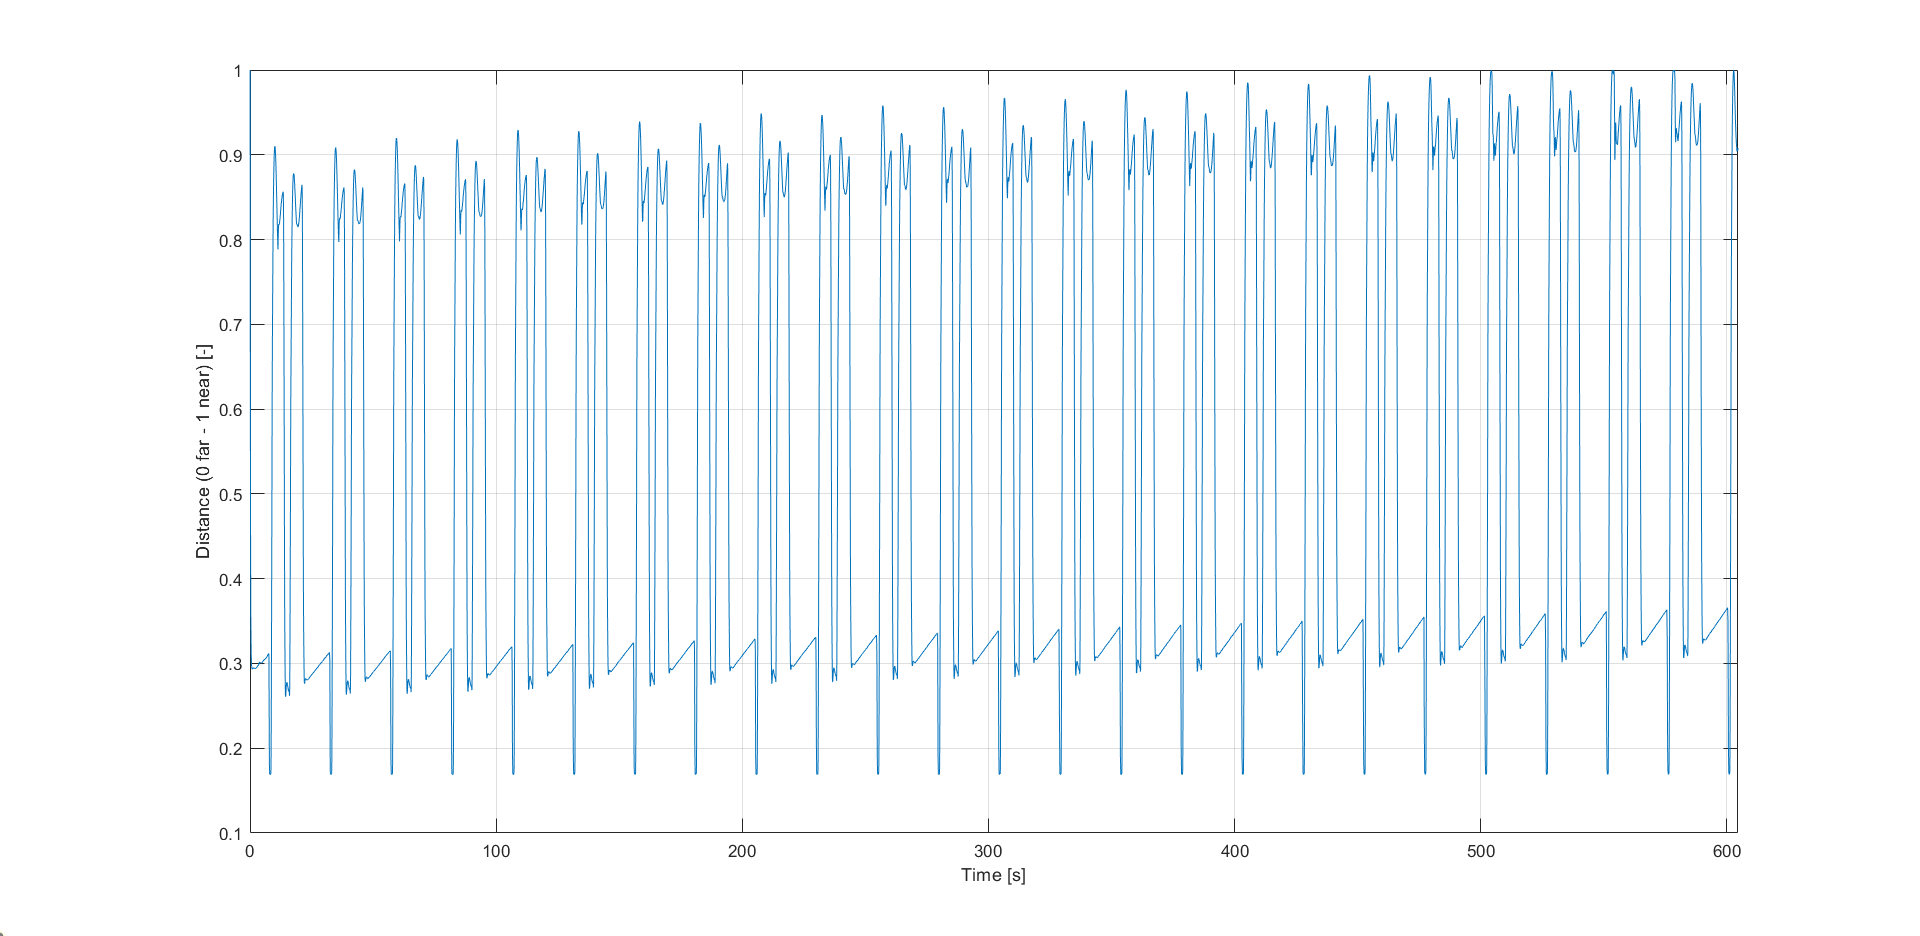
\includegraphics[width=\linewidth]{images/chapter3/distEllipse_wear_no20.png}
    \caption{Distance of (Fx, Fy) from the ellipse}
    \label{fig:res_distEllipse_stressNo20}
\end{figure}

\begin{figure}[h!]
    \centering
    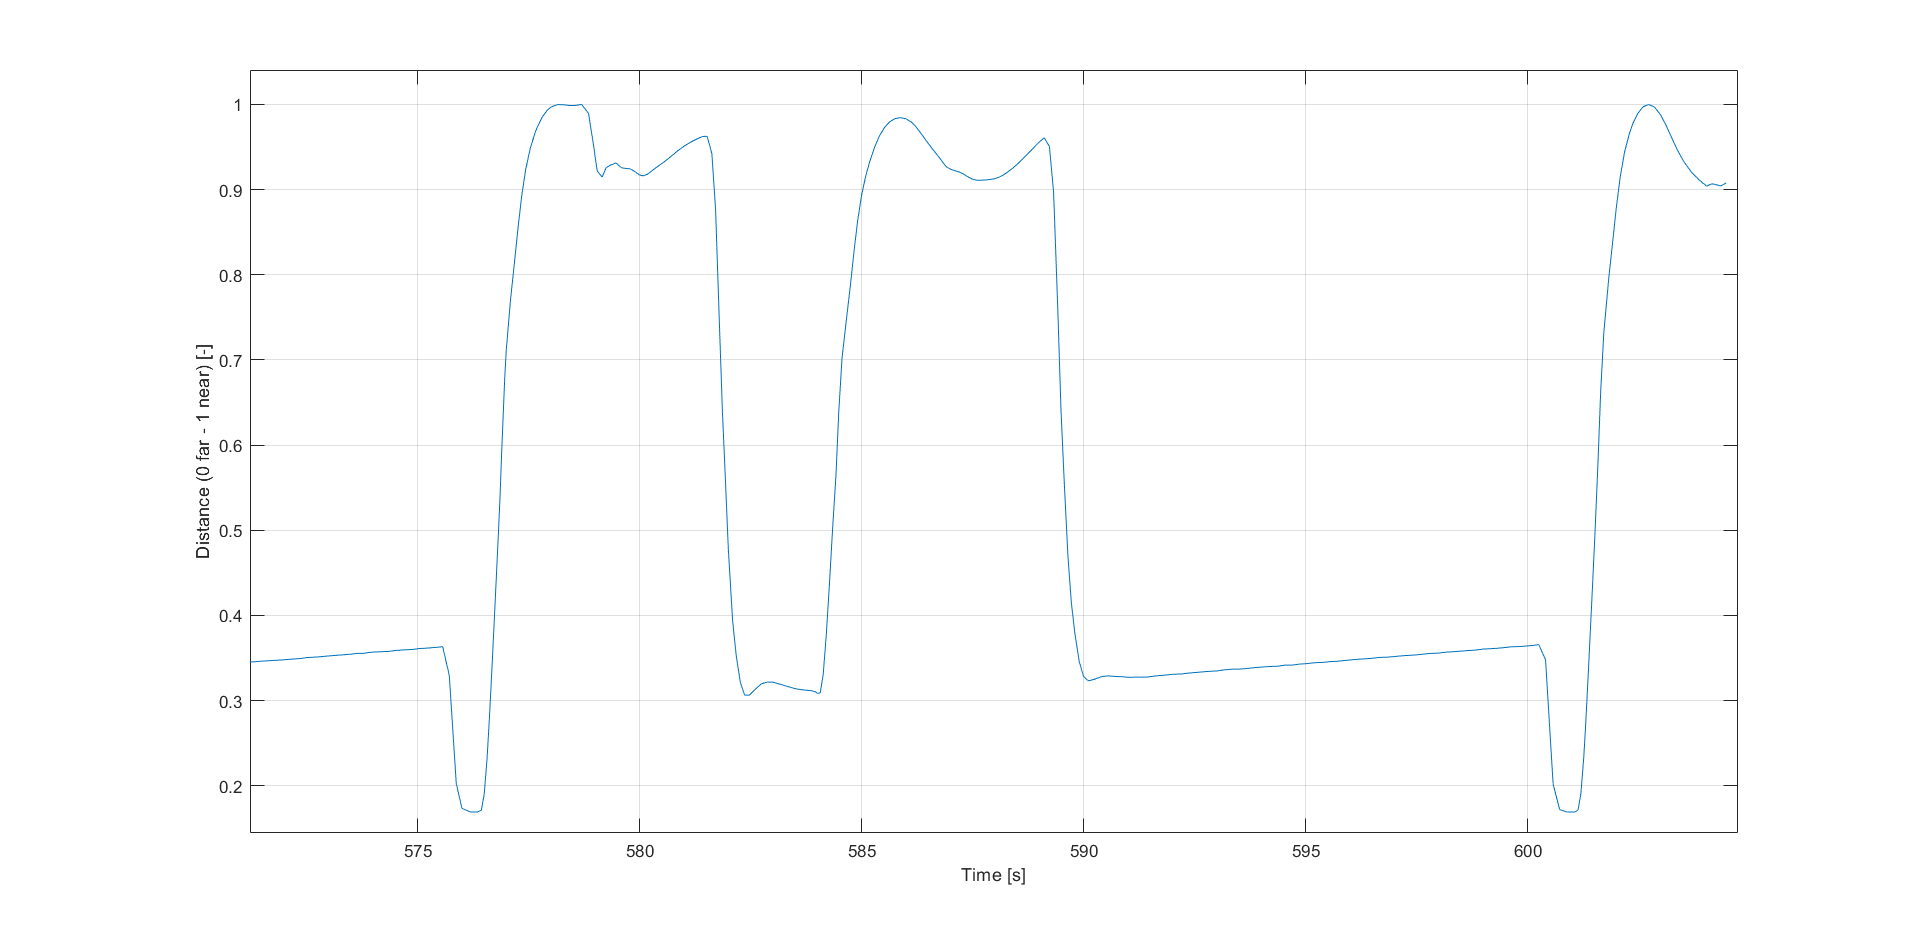
\includegraphics[width=\linewidth]{images/chapter3/distEllipse_wear_no20_det.png}
    \caption{Distance of (Fx, Fy) from the ellipse - detail of the last lap}
    \label{fig:res_distEllipse_stressNo20_det}
\end{figure}

\begin{figure}[h!]
    \centering
    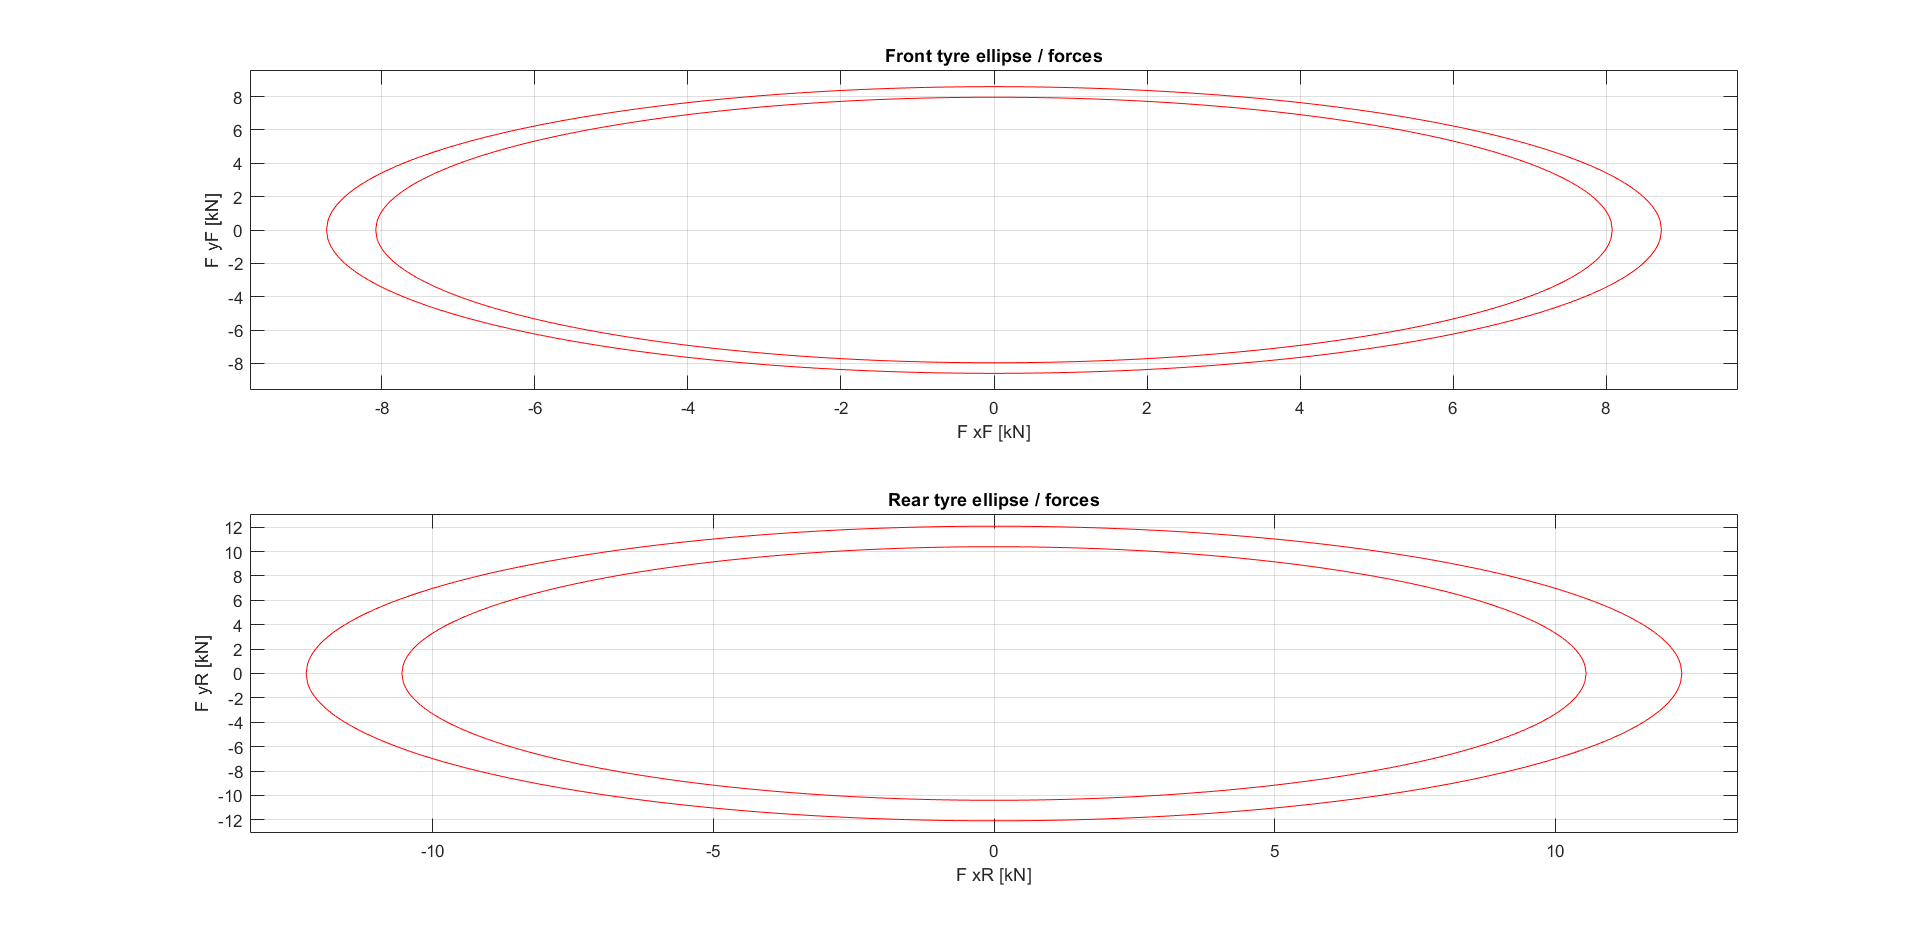
\includegraphics[width=\linewidth]{images/chapter3/wear_stress_no20.png}
    \caption{Ellipse reduction due to the wear - 14\% less on rear tyre - 7\% loss on front tyre}
    \label{fig:res_wear_stressNo20}
\end{figure}

\subsection{Second run: slipstreaming for 20 laps}
This test ends since the value of error reached the limit of 2 meters. \\Figure \ref{fig:res_distEllipse_stress20} shows the distance of the pair (Fx,Fy) on the friction ellipse with a value 0/1, where 0 represents "far" from the ellipse and "1" represents on the border of the ellipse; it can be seen that going towards the final seconds the ellipse is going to be saturated. At that time the vehicle had done 15 laps. Also the reduction of the ellipses, that corresponds to a loss in performances since lower forces and thus velocities can be handled, is reported in figures \ref{fig:res_wear_stress20}

\begin{figure}[h!]
    \centering
    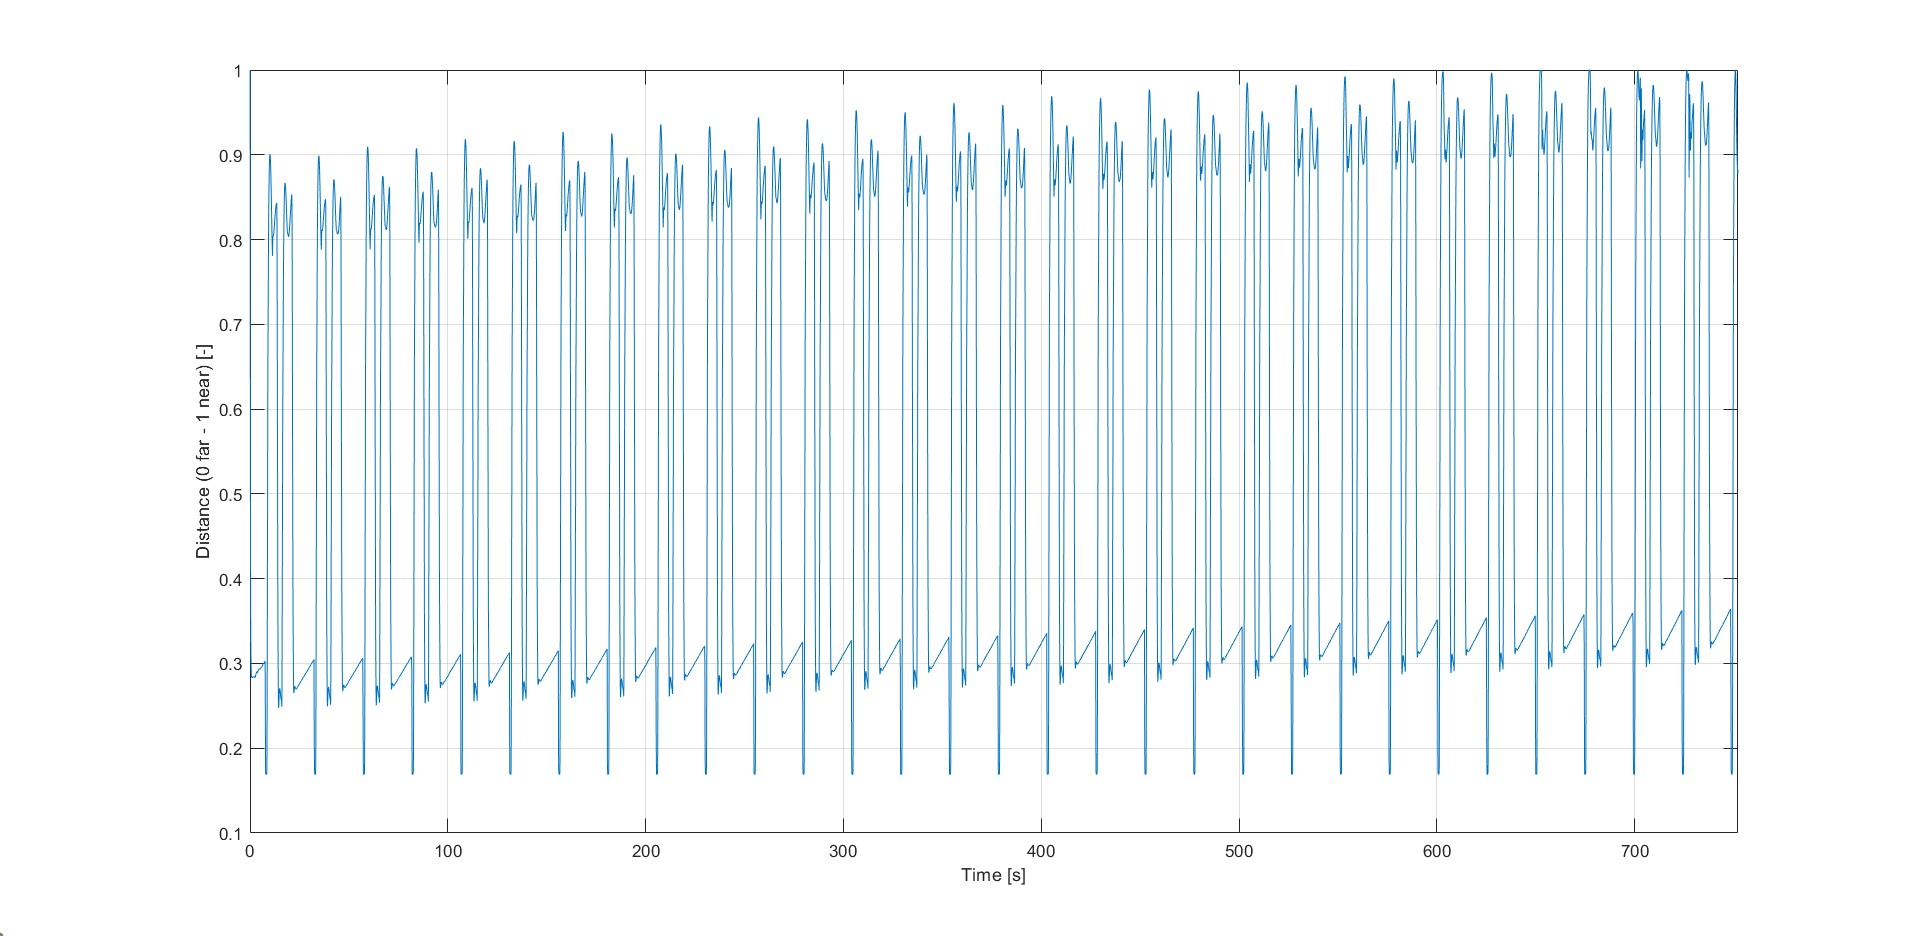
\includegraphics[width=\linewidth]{images/chapter3/distEllipse_wear_20.png}
    \caption{Distance of (Fx, Fy) from the ellipse}
    \label{fig:res_distEllipse_stress20}
\end{figure}

\begin{figure}[h!]
    \centering
    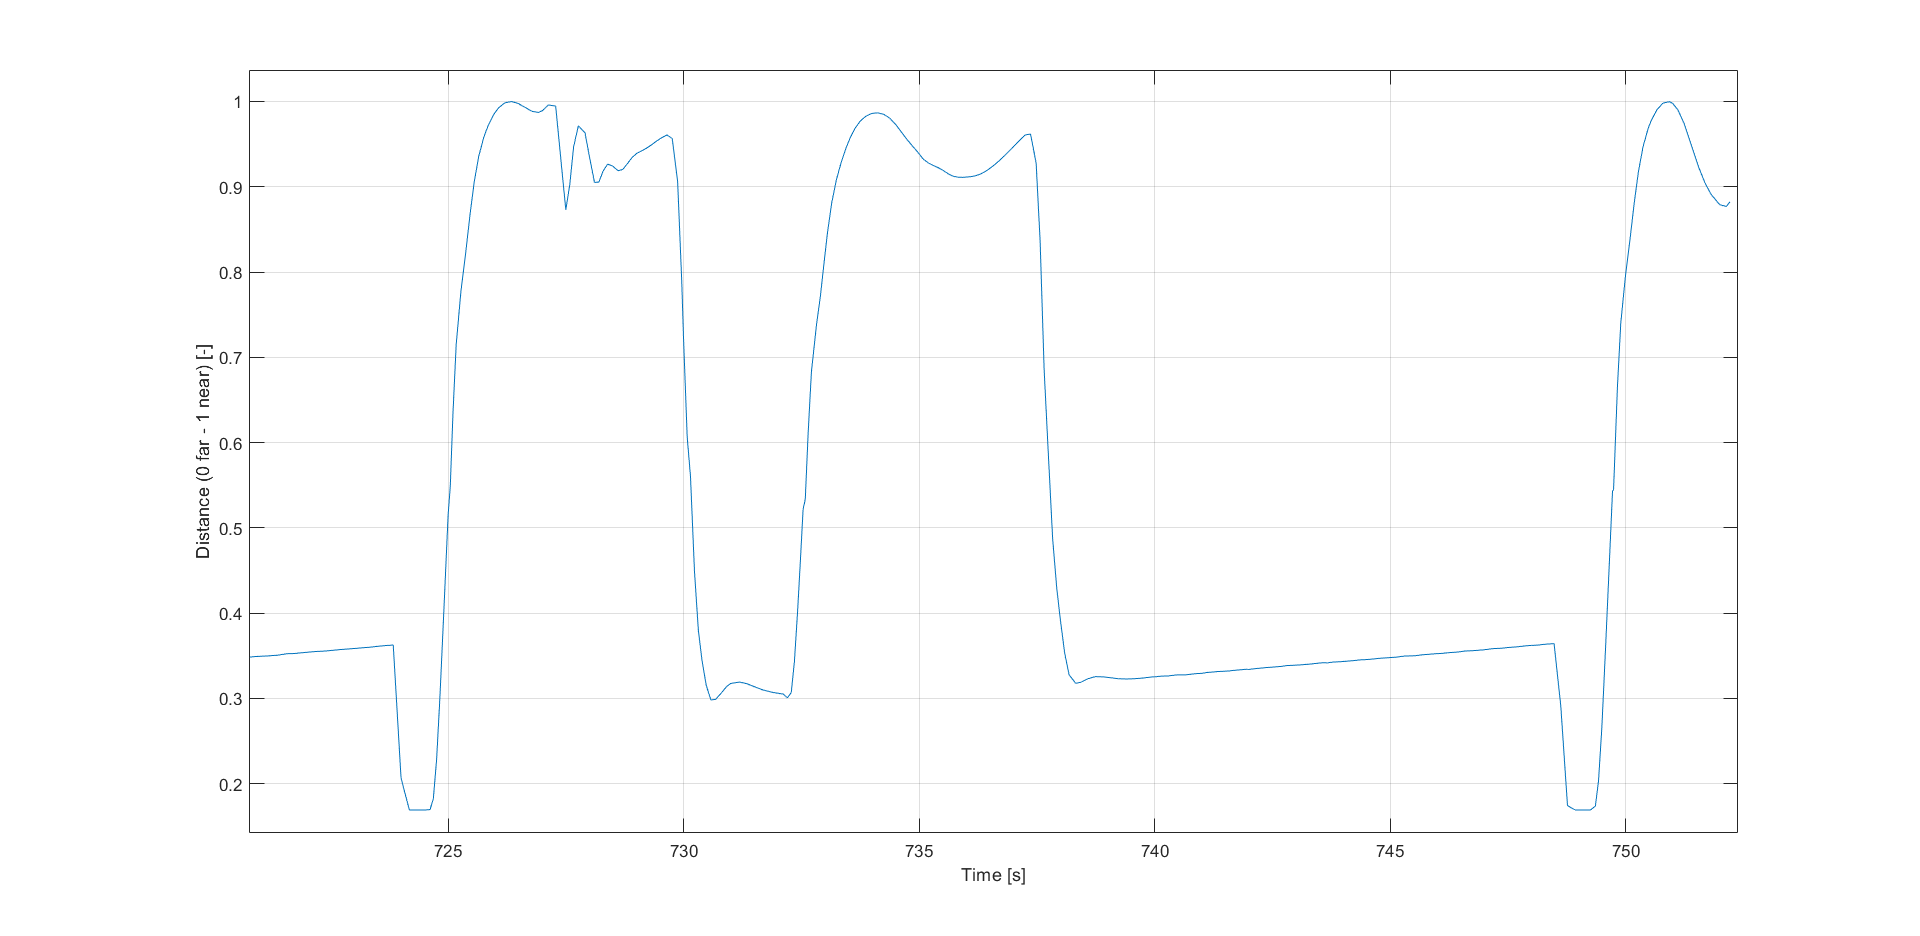
\includegraphics[width=\linewidth]{images/chapter3/distEllipse_wear_20_det.png}
    \caption{Distance of (Fx, Fy) from the ellipse - detail of the last lap}
    \label{fig:res_distEllipse_stress20_det}
\end{figure}

\begin{figure}[h!]
    \centering
    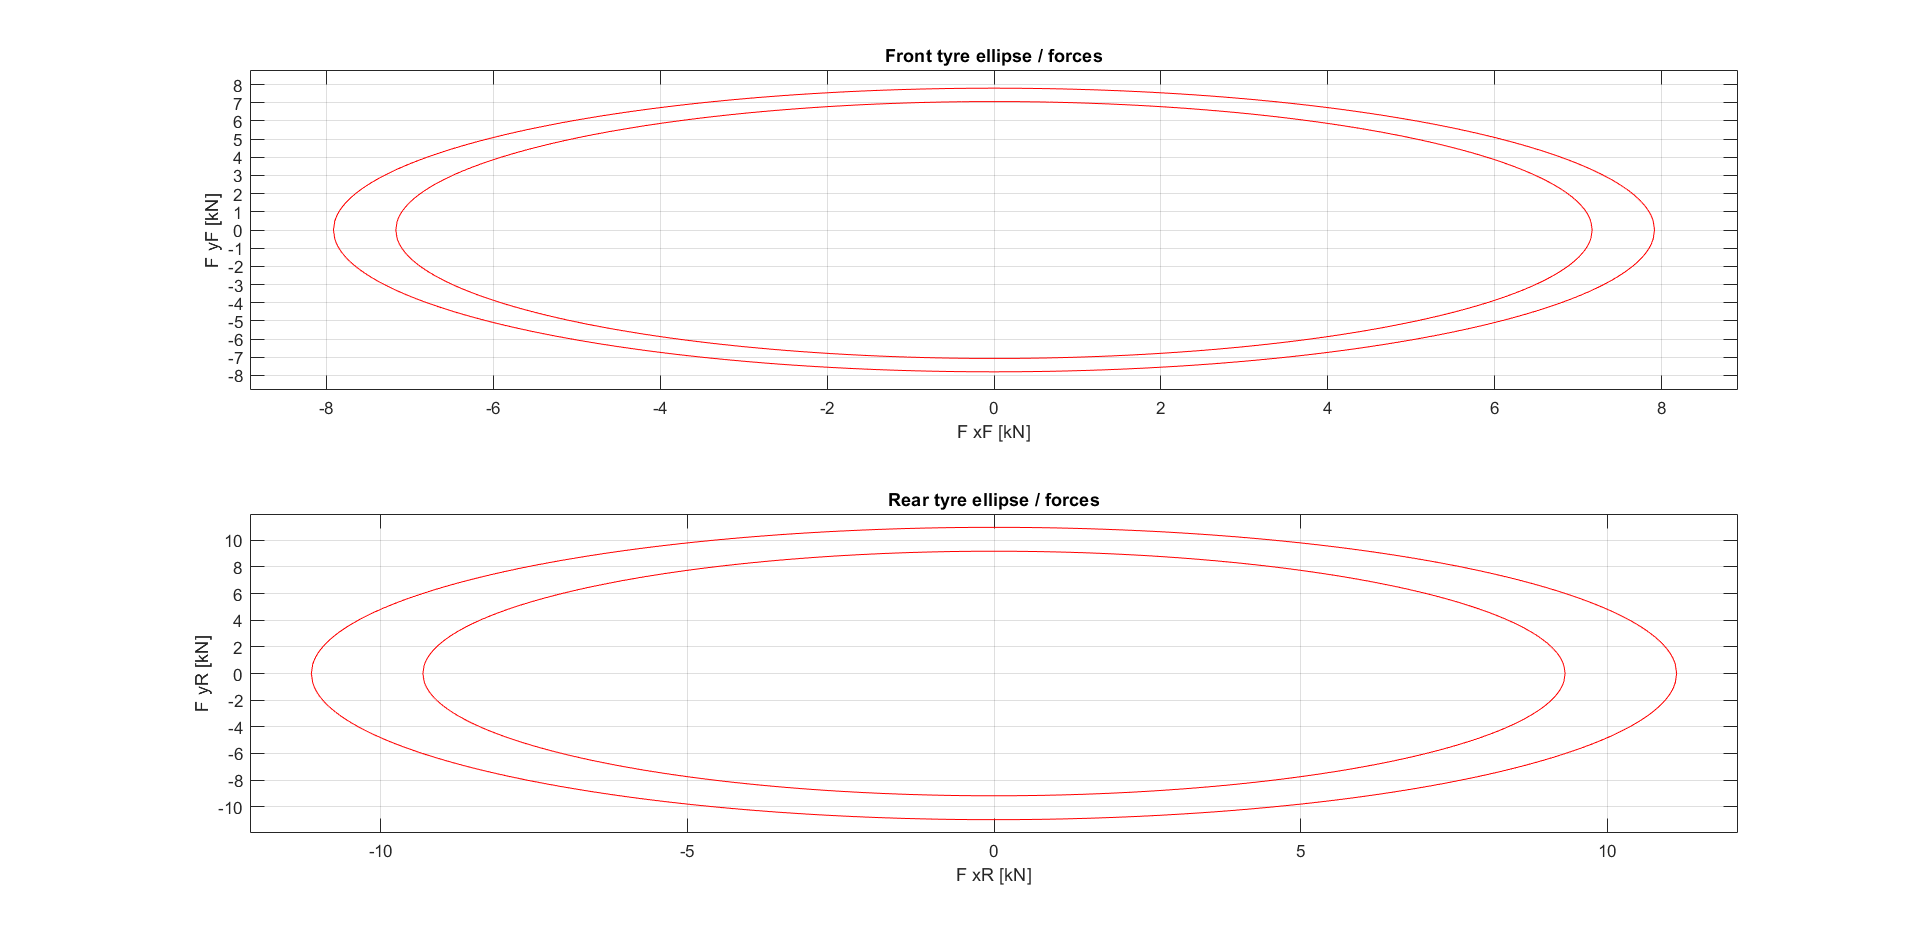
\includegraphics[width=\linewidth]{images/chapter3/wear_stress_20.png}
    \caption{Ellipse reduction due to the wear - 16\% less on rear tyre - 9\% loss on front tyre}
    \label{fig:res_wear_stress20}
\end{figure}

\subsection{Third run: slipstreaming for 10 laps}
This test ends since the value of error reached the limit of 2 meters. At that time the vehicle had done 14 laps. Coherently with expected the result is not as good as the second simulation but it's good enough to say that there's a significant improvement in performances.

\subsection{Comparisons}
It is evident that slipstreaming leads to benefits in the performances of the vehicle. Indeed, without it the vehicle loses the capability of handling the requested velocities after 12 laps, while having slipstream ON all the race long leads to a longer race, 15 laps. Altough this is just a qualitatively result, since is not actually possible to do all the race slipstreaming, from third simulation, as already said, can be seen that also slipstreaming for half of the time leads to increase in the performances since 14 laps are possible.
\\\\What happens is that with slipstreaming, since aerodynamic forces are lower, to obtain the same velocity less force is necessary. This force reduction leads to have less wear and thus the ellipse reduction is slower then when not slipstreaming. For this reason higher velocities can be handled for more time before the ellipse reaches the point in which such velocities become unfeasible. To be complete, as can be seen from previous figures, this point is around 15\% of wear for rear tyre and 8\% for front tyre. 
\\\\Figure \ref{fig:res_Fx_comparison} actually shows how during the slipstreaming simulation the longitudinal force is lower than in the simulation with no slipstreaming

\begin{figure}[h!]
    \centering
    \includegraphics[width=\linewidth]{images/chapter3/fx.png}
    \caption{FxR comparison between no slipstreaming and slipstreaming for a simulation snapshot}
    \label{fig:res_Fx_comparison}
\end{figure}

\section{20 laps test}
During this test the vehicle follows the desired trajectory for 20 laps, that is how long the real race lasts. During this 20 laps the velocity profile is scaled according to the mean tyre wear following the formula
\begin{equation*}
\begin{aligned}
v_{ref\_h}(s) = v_{ref}(s) \frac{1}{1 + K_{wear\_vel}h_{mean}}\\\\
h_{mean} = \frac{h_F + h_R}{2}\\\\
\end{aligned}
\end{equation*}
Where $h_F$ and $h_R$ are the tyre wears of respectively front and rear tyres, $K_{wear\_vel}$ is a set of two different parameters, one to be used during slipstreaming and one to use while not; s is the curvilinear abscissa.
\\The objective and the way in which these parameters have been chosen is that the vehicle must follow the trajectory for 20 laps, with the error been bounded, at the maximum velocity that can be handled according to the percentage of wear.
\\The analysis is focused on showing how slipstreaming impacts on 
\begin{itemize}
    \item Race time
    \item Tyre wears
    \item Fuel consumption
    \item Maximum velocity difference from first and last lap
\end{itemize}

\subsection{20 laps - no slipstreaming}
The simulation ended correctly after $T_{race}$ = 1010.495 [s] that corresponds to an average lap time $T_{lap}$ = 50.525 [s].
\\Peak velocity decreases from 88 [m/s] to 84.2 [m/s] (figure \ref{fig:_res_20laps_noS_vel}).
\\Maximum lateral forces reduction (figure \ref{fig:_res_20laps_noS_fy}) is of 24.05\% on rear tyre and 14.92\% on the front tyre.
\\Fuel consumption is 57.91 [kg] out of 58 [kg], thus 0.09 [kg] remaining (figure \ref{fig:_res_20laps_noS_fuel}).

\begin{figure}[h!]
    \centering
    \includegraphics[width=\linewidth]{images/chapter3/20laps_vel_noS.png}
    \caption{Peak velocity reduction - no slipstreaming}
    \label{fig:_res_20laps_noS_vel}
\end{figure}

\begin{figure}[h!]
    \centering
    \includegraphics[width=\linewidth]{images/chapter3/20laps_ellipse_noS.png}
    \caption{Ellipse (maximum lateral forces) reduction - no slipstreaming}
    \label{fig:_res_20laps_noS_fy}
\end{figure}

\begin{figure}[h!]
    \centering
    \includegraphics[width=\linewidth]{images/chapter3/20laps_fuel_noS.png}
    \caption{Fuel consumption (mass reduction) - no slipstreaming}
    \label{fig:_res_20laps_noS_fuel}
\end{figure}

\subsection{20 laps - slipstreaming}
The simulation ended correctly after $T_{race}$ = 1001.475 [s] that corresponds to an average lap time $T_{lap}$ = 50,074 [s].
\\Peak velocity decreases from 88 [m/s] to 85.7 [m/s] (figure \ref{fig:_res_20laps_S_vel}).
\\Maximum lateral forces reduction (figure \ref{fig:_res_20laps_S_fy}) is of 22.07\% on rear tyre and 13.82\% on the front tyre.
\\Fuel consumption is 51.71 [kg] out of 58 [kg], thus 6.29 [kg] remaining (figure \ref{fig:_res_20laps_S_fuel}).

\begin{figure}[h!]
    \centering
    \includegraphics[width=\linewidth]{images/chapter3/20laps_vel_S.png}
    \caption{Peak velocity reduction - slipstreaming}
    \label{fig:_res_20laps_S_vel}
\end{figure}

\begin{figure}[h!]
    \centering
    \includegraphics[width=\linewidth]{images/chapter3/20laps_ellipse_S.png}
    \caption{Ellipse (maximum lateral forces) reduction - slipstreaming}
    \label{fig:_res_20laps_S_fy}
\end{figure}

\begin{figure}[h!]
    \centering
    \includegraphics[width=\linewidth]{images/chapter3/20laps_fuel_S.png}
    \caption{Fuel consumption (mass reduction) - slipstreaming}
    \label{fig:_res_20laps_S_fuel}
\end{figure}

\subsection{Comparisons}
From the results it can be seen that
\begin{itemize}
    \item Total race time is reduced by around 9 seconds, so an average of 0.5 seconds per lap that could be significant in a race
    \item Peak velocity increases by the 2\%, from 84.2 [m/s] to 85.7 [m/s], this is due to the fact that since tyres wear increasing is slower, higher velocities can be handled for more time
    \item Maximum lateral forces reduction decreases by 2\% on the rear wheel and by 1\% on the front one. 
    \item Fuel consumption loss is significantly less, 0.09 [kg] of fuel remaining in the case of no-slipstreaming and 6.29 [kg] while slipstreaming, around 6 [kg] saved
\end{itemize} 


\section{Sensitivity to tyre wear error}
A further test that has been executed wants to show how an error on the estimation of tyre wear impacts on the lap time. Starting from the effective value used for tyre wear, we made some changes by increasing and decreasing it with the goal of obtaining a final loss on the friction ellipse respectively of around +5\% and -5\% to simulate how an error of the estimation may impact on the final results.
In the following we show the conditions on which each simulation has been run and the respective race and lap time. Notice that a slightly different scaling in velocity due to wear has been applied.

\begin{itemize}
    \item   Simulation with loss higher by 5\%
            \begin{itemize}
                \item Loss on rear ellipse 29\%
                \item Race time 1029.7 [s]
                \item Lap time 51.485 [s]
            \end{itemize} 
    \item   Reference simulation
            \begin{itemize}
                \item Loss on rear ellipse 24.5\%
                \item Race time 1019.510 [s]
                \item Lap time 50.976 [s] 
            \end{itemize} 
    \item Simulation with loss lower by 5\%  
        \begin{itemize}
            \item Loss on rear ellipse 20.2\%
            \item Race time 1010.835 [s]
            \item Lap time 50.542 [s]
        \end{itemize}
\end{itemize}

From the results it can be seen that an error on estimation of tyre wear of around 5\% has an impact of less than 1\% on the lap time. So, we can conclude that having a small error on the estimation with respect to the real value may not be so critical.




\chapter{Appendix A}
In this section we will define the values given to the different parameters of the model. 

\begin{equation*}
\begin{aligned}
\text{Parameters of lateral Pacejka tyre model}\\
a0 = 1.47 [-] \text{--------Shape factor}\\
a1 = 0 [1/kN] \text{--------Load influence on lateral friction coefficient (*1000)}\\
a2 = 2050 [-] \text{--------Lateral friction coefficient (*1000)}\\
a3 = 2500 [N/deg] \text{--------Change of stiffness with slip}\\
a4 = 10 [kN] \text{--------Change of progressivity of stiffness / load}\\
a5 = 0 [\%/deg/100] \text{--------Camber influence on stiffness}\\
a6 = 0 [-] \text{--------Curvature change with load}\\
a7 = -2 [-] \text{--------Curvature factor}\\
a8 = 0 [deg/kN] \text{--------Load influence on horizontal shift}\\
a9 = 0 [deg] \text{--------Horizontal shift at load = 0 and camber = 0}\\
a10 = 0 [-] \text{--------Camber influence on horizontal shift}\\
a11 = 0 [N] \text{--------Vertical shift}\\
a12 = 0 [N] \text{--------Vertical shift at load = 0}\\
a13 = 0 [N/deg/kN] \text{--------Camber influence on vertical shift, load dependent}\\
a14 = 0 [N/deg] \text{--------Camber influence on vertical shift}\\
a15 = 0 [1/deg] \text{--------Camber influence on lateral friction coefficient}\\
a16 = 0 [-] \text{--------Curvature change with camber}\\
a17 = 0 [-] \text{-------- 	Curvature shift}\\\\
\gamma = 0 [rad] \text{--------Camber angle}\\\\
\text{Parameters of longitudinal tyre model - only the ones used}\\
b1 = 0 [1/kN] \text{--------Load influence on longitudinal friction coefficient (*1000)}\\
b2 = 2080 [-] \text{--------Longitudinal friction coefficient (*1000)}\\
b11 = 0 [N] \text{--------Vertical shift}\\
b12 = 0 [N] \text{--------Vertical shift at load = 0}\\
\end{aligned}
\end{equation*}

\begin{equation*}
\begin{aligned}
m_{vehicle} = 590 [kg] \text{--------Mass of the vehicle}\\
m_{fuel} = 58 [kg] \text{--------Mass of the fuel}\\
m_{passenger} = 70 [kg] \text{--------Mass of the passenger}\\
m_T = m_{vehicle} + m_{fuel}+ m_{passenger} \\
g = 9.81 [\frac{m}{s^2}] \text{--------Gravity acceleration}\\
l_F = 0.414 [-] \text{--------Distribution of load on the front wheel}\\
l_R = 0.586 [-] \text{---------Distribution of load on the rear wheel}\\
C_F = 100000 [N/rad] \text{---------Cornering stiffness coefficient of front wheel}\\ 
C_R = 120000 [N/rad] \text{---------Cornering stiffness coefficient of rear wheel}\\ 
a = 1.767 [m] \text{--------Distance between center of vehicle and front wheel}\\
b = 1.353 [m] \text{--------Distance between center of vehicle and rear wheel}\\
L = a + b [m] \text{--------Wheelbase}\\
I_T = 606 [kg m^2] \text{--------Moment of Inertia of the vehicle}\\\\
\end{aligned}
\end{equation*}

\begin{equation*}
\begin{aligned}
C_x = 0.725 [-] \text{--------Drag coefficient}\\
C_z = 0.778 [-] \text{--------Lift coefficient}\\
rho_{noslipstream} = 1.225 [\frac{kg}{m^3}] \text{--------Density of air without slipstream effect}\\
rho_{slipstream} = 0.8 [\frac{kg}{m^3}] \text{--------Density of air with slipstream effect}\\
S = 1 [m^2] \text{--------Area on which the air goes through}\\\\
\end{aligned}
\end{equation*}

\begin{equation*}
\begin{aligned}
C_{fuel} = 2.1x10^{-7} [\frac{s^2}{m^2}] \text{--------Fuel consumption coefficient}\\\\
K_{wear} = 1.8*10^{-17} [\frac{m^3s^3}{kg^2}] \text{--------Tyre wear parameter}\\
K_{wear\_high} = 2.4*10^{-17} [\frac{m^3s^3}{kg^2}] \text{--------High tyre wear parameter for relative error simulation}\\
K_{wear\_low} = 1.3*10^{-17} [\frac{m^3s^3}{kg^2}] \text{--------Low tyre wear parameter for relative error simulation}\\
K_{wear\_vel\_noslipstream} = 10^{-5.05} [m^{-3}]
K_{wear\_vel\_slipstream} = 10^{-5.25} [m^{-3}]
K_{wear\_vel\_0\_relError} = 10^-4.9 [m^{-3}]
\text{--------Tyre wear parameter}\\
Tyre Contact Area Front = 0.072137 [m^2] \text{--------Contact area between front tyre and asphalt}\\
Tyre Contact Area Rear = 0.082758 [m^2] \text{--------Contact area between rear tyre and asphalt}\\\\
\end{aligned}
\end{equation*}

\begin{equation*}
\begin{aligned}
w_1 = 10^{-4.5} [-] \text{--------Parameter to scale ellipse due to wear}\\
w_2 = 1 [-] \text{--------Parameter to scale ellipse due to wear}
\end{aligned}
\end{equation*}

\end{document}
